\documentclass[xcolor=pdftex,dvipsnames,table,mathserif]{beamer}
%\documentclass[handout,xcolor=pdftex,dvipsnames,table,mathserif]{beamer}
\usepackage{subfigure}
\usepackage{amsbsy}
\usepackage{tikz}
\usetikzlibrary{arrows}
\usepackage{amsmath,graphicx,dsfont,color}
\usepackage{amsfonts}
\usepackage{amssymb}
\usepackage{array}

\bibliographystyle{apalike}

\setbeamertemplate{bibliography item}{\insertbiblabel}
\setbeamertemplate{bibliography entry title}{}
\setbeamertemplate{bibliography entry location}{}
\setbeamertemplate{bibliography entry note}{}

%Definitiona

\newcommand{\x}{\mathbf{x}}
\newcommand{\X}{\mathbf{X}}
\newcommand{\W}{\mathbf{W}} %Weight
\newcommand{\bais}{\mathbf{b}}%Bais
\newcommand{\act}{\texttt{g}}%Activation
\newcommand{\loss}{L}
\newcommand{\pdata}{\hat{p}_{\texttt{data}}}
\newcommand{\nsize}{n}
\newcommand{\param}{\boldsymbol{\theta}}
\newcommand{\featmap}{\boldsymbol{\phi}}
\newcommand{\EV}{\mathbb{E}}







\usepackage{physics}

\graphicspath{{../graphics/}}

\AtBeginSection[]{
  \begin{frame}{Contents}
  \tableofcontents[currentsection, hideothersubsections]
  \end{frame}
}

\AtBeginSubsection[]{
  \begin{frame}{Contents}
  \tableofcontents[currentsection, subsectionstyle=show/shaded/hide]
  \end{frame}
}

\setbeamertemplate{footline}[frame number]{}
\setbeamertemplate{navigation symbols}{}
\setbeamertemplate{section in toc}[square]
\setbeamertemplate{items}[square]

\title{Artificial neural networks and backpropagation}
\author{E. Decencière}
\date{MINES ParisTech\\
  PSL Research University\\
  Center for Mathematical Morphology
}
\titlegraphic{
\includegraphics[height=1.7cm]{logoemp}}

\useinnertheme{rounded}
\usecolortheme{rose}

%%%%%%%%%%%%%%%%%%%%%%%%%%%%%%%%%%%%%%%%%%%%%%%%%%
%%%%%%%%%%%%%%%%%%%%%%%%%%%%%%%%%%%%%%%%%%%%%%%%%%
\begin{document}
\begin{frame}
\titlepage
\end{frame}

\frame{
\frametitle{Contents}
\tableofcontents[hidesubsections]
}


%%%%%%%%%%%%%%%%%%%%%%%%%%%%%%%%%%%%%%%%%%%%%%%%%%
\section{Introduction}
%%%%%%%%%%%%%%%%%%%%%%%%%%%%%%%%%%%%%%%%%%%%%%%%%%

\frame{
\frametitle{Artificial neural networks and deep learning history}


\begin{block}{}
  For a very complete state of the art on deep learning, see the overview by Schmidhuber \cite{schmidhuber_deep_2015}.
\end{block}

\begin{itemize}[<+->]
\item 1958: Rosenblatt's perceptron \cite{rosenblatt_perceptron:_1958}
\item 1979: Neocognitron (convolutional neural network architecture) \cite{fukushima_neural_1979,fukushima_neocognitron:_1980}
\item 1980's: the backpropagation algorithm (see, for example, the work of LeCun \cite{lecun_procedure_1985})
\item 2006-: CNN implementations using Graphical Processing Units (GPU): up to a 50 speed-up factor.
\item 2012: Imagenet image classification won by a CNN with AlexNet \cite{krizhevsky_imagenet_2012}.

\end{itemize}

}

%%%%%%%%%%%%%%%%%%%%%%%%%%%%%%%%%%%%%%%%%%%%%%%%%%
\section{Artificial neuron}
%%%%%%%%%%%%%%%%%%%%%%%%%%%%%%%%%%%%%%%%%%%%%%%%%%

\frame{
\frametitle{Biological neuron}

\begin{figure}
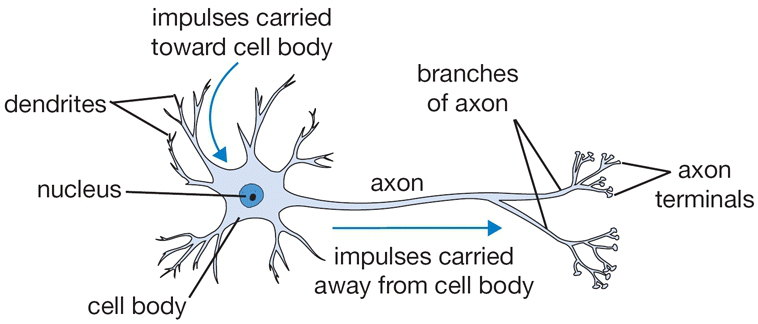
\includegraphics[height=3cm]{neuron}
\end{figure}

\begin{itemize}[<+->]
\item The human brain contains 100 billion ($10^{11}$) neurons
\item A human neuron can have several thousand dendrites
\item The neuron sends a signal through its axon if during a given interval of time the net input signal (sum on excitatory and inhibitory signals received through its dendrites) is larger than a threshold.
\end{itemize}

}

%%%%%%%%%%%%%%%%%%%%%%%%%%%%%%%%%%%%%%%%%%%%%%%%%%

\frame{
\frametitle{Artificial neuron}

\begin{figure}
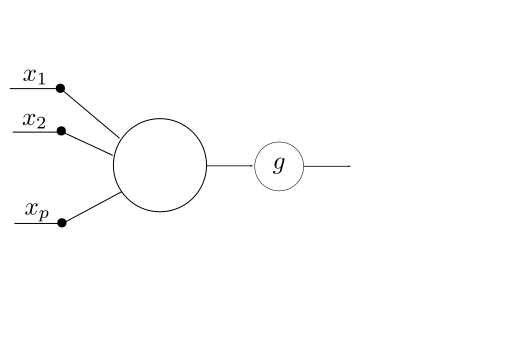
\includegraphics[height=3cm]{neurone_general}
\end{figure}

\begin{block}{General principle}
An artificial neuron takes $p$ inputs $\{x_i\}_{1 \leq i \leq p}$, combines them to obtain a single value, and applies an \alert{activation function} $\act$ to the result.
\end{block}

\pause

\begin{itemize}
\item The first artificial neuron model was proposed by \cite{mcculloch_logical_1943}
\item Input and output signals were binary
\item Input dendrites could be inhibitory or excitatory
\end{itemize}

}

%%%%%%%%%%%%%%%%%%%%%%%%%%%%%%%%%%%%%%%%%%%%%%%%%%

\frame{
  \frametitle{Modern artificial neuron}

  \begin{figure}
    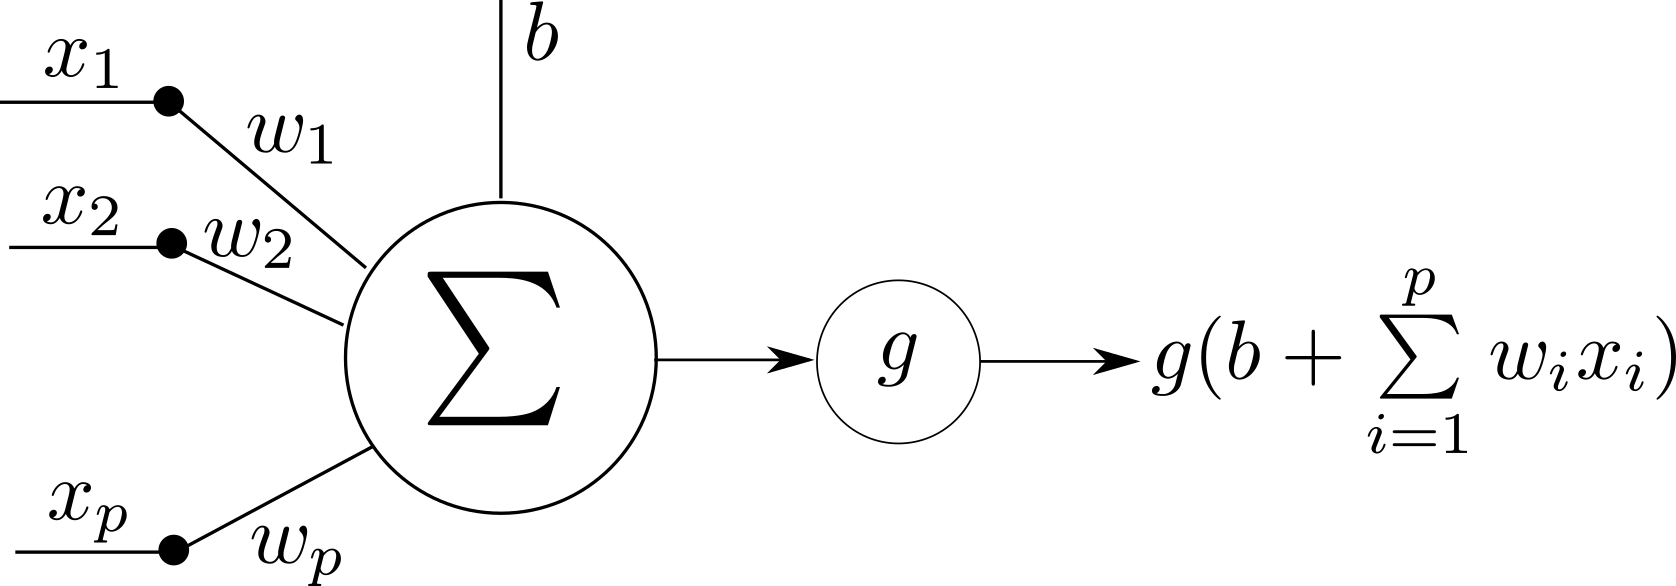
\includegraphics[height=3cm]{neurone}
  \end{figure}

  \begin{itemize}
  \item The neuron computes a linear combination of the \alert{inputs} $x_i$
    \begin{itemize}
    \item The \alert{weights} $w_i$ are multiplied with the inputs
    \item The \alert{bias} $b$ can be interpreted as a threshold on the sum
    \end{itemize}

  \item The \alert{activation function} $\act$ somehow decides, depending on its input, if a signal (the neuron's \alert{activation}) is produced
  \end{itemize}


}

%%%%%%%%%%%%%%%%%%%%%%%%%%%%%%%%%%%%%%%%%%%%%%%%%%
\subsection{Activation functions}
%%%%%%%%%%%%%%%%%%%%%%%%%%%%%%%%%%%%%%%%%%%%%%%%%%

%%%%%%%%%%%%%%%%%%%%%%%%%%%%%%%%%%%%%%%%%%%%%%%%%%

\frame{
  \frametitle{The role of the activation function}

  \begin{figure}
    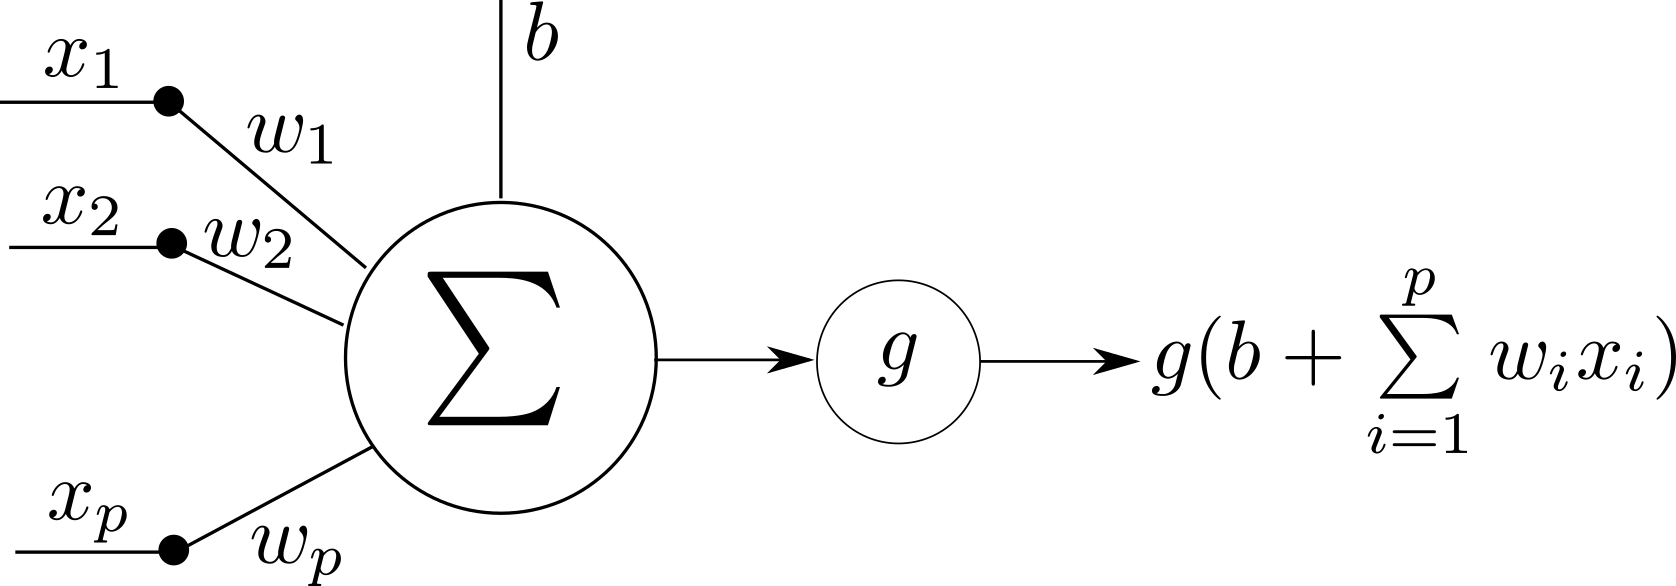
\includegraphics[height=3cm]{neurone}
  \end{figure}

  \begin{itemize}
  \item The initial idea behind the activation function is that it works somehow as a gate
  \item If its input in ``high enough'', then the neuron is activated, i.e. a signal (other than zero) is produced
  \item It can be interpreted as a source of abstraction: information considered as unimportant is ignored
  \end{itemize}

}

%%%%%%%%%%%%%%%%%%%%%%%%%%%%%%%%%%%%%%%%%%%%%%%%%%

\frame{
  \frametitle{Activation: binary}

  \begin{columns}
    \begin{column}{.5\textwidth}
      \[
      \act(x)=
      \begin{cases}
        1,& \text{if } x > 0\\
        0,              & \text{otherwise}
      \end{cases}
      \]

    \end{column}

    \begin{column}{.5\textwidth}
      \begin{figure}
        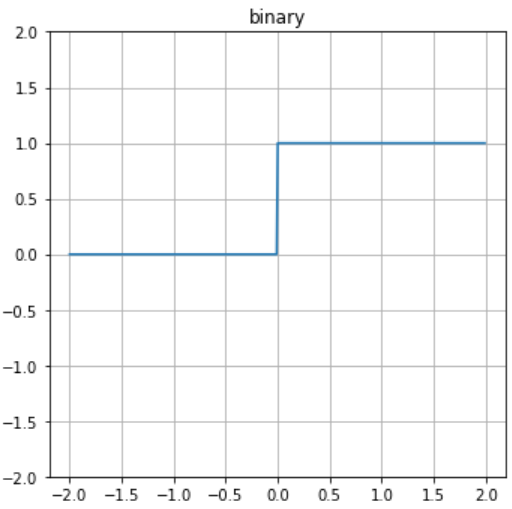
\includegraphics[width=.8\textwidth]{act_bin.png}
      \end{figure}


    \end{column}
  \end{columns}

  \begin{block}{Remarks}
    \begin{itemize}
    \item Biologically inspired
    \item[+] Simple to compute
    \item[+] High abstraction
    \item[-] Gradient nil except on one point
    \item \alert{In practice, almost never used}
    \end{itemize}
  \end{block}


}

%%%%%%%%%%%%%%%%%%%%%%%%%%%%%%%%%%%%%%%%%%%%%%%%%%

\frame{
  \frametitle{Activation: sigmoid}

  \begin{columns}
    \begin{column}{.5\textwidth}
      \[
      \act(x)= \frac{1}{1 + e^{-x}}
      \]
    \end{column}

    \begin{column}{.5\textwidth}
      \begin{figure}
        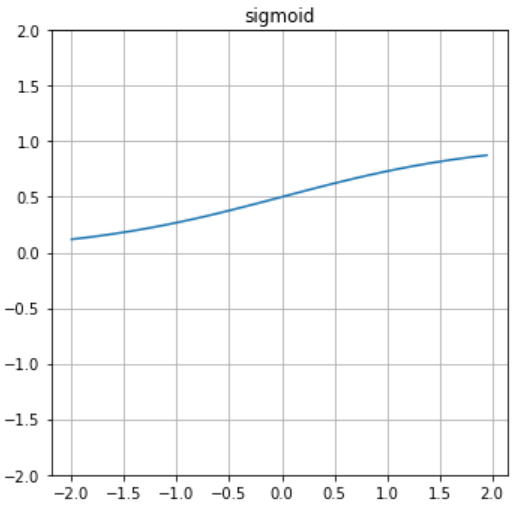
\includegraphics[width=.8\textwidth]{act_sigm.png}
      \end{figure}


    \end{column}
  \end{columns}

  \begin{block}{Remarks}
    \begin{itemize}
    \item[+] Similar to binary activation, but with usable gradient
    \item[-] However, gradient tends to zero when input is far from zero
    \item[-] More computationally intensive
    \end{itemize}
  \end{block}



}

%%%%%%%%%%%%%%%%%%%%%%%%%%%%%%%%%%%%%%%%%%%%%%%%%%

\frame{
  \frametitle{Activation: hyperbolic tangent}

  \begin{columns}
    \begin{column}{.5\textwidth}
      \[
      \act(x)= \frac{e^x - e^{-x}}{e^x + e^{-x}}
      \]
    \end{column}

    \begin{column}{.5\textwidth}
      \begin{figure}
        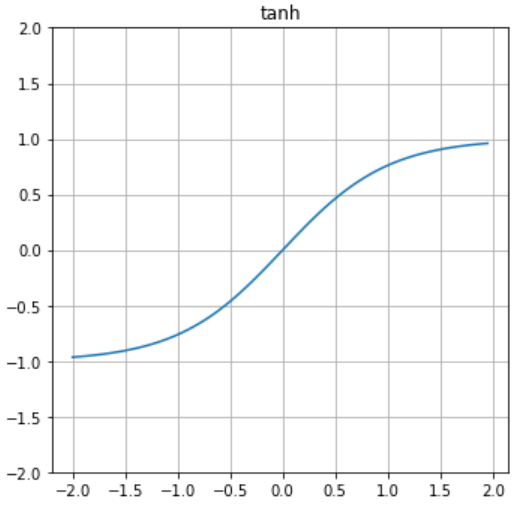
\includegraphics[width=.8\textwidth]{act_tanh.png}
      \end{figure}


    \end{column}
  \end{columns}

  \begin{block}{Remarks}
    \begin{itemize}
    \item Similar to sigmoid
    \end{itemize}
  \end{block}



}


%%%%%%%%%%%%%%%%%%%%%%%%%%%%%%%%%%%%%%%%%%%%%%%%%%

\frame{
  \frametitle{Activation: rectified linear unit (ReLU)}

  \begin{columns}
    \begin{column}{.5\textwidth}
      \[
      \act(x)=
      \begin{cases}
        x,& \text{if } x > 0\\
        0,              & \text{otherwise}
      \end{cases}
      \]
    \end{column}

    \begin{column}{.5\textwidth}
      \begin{figure}
        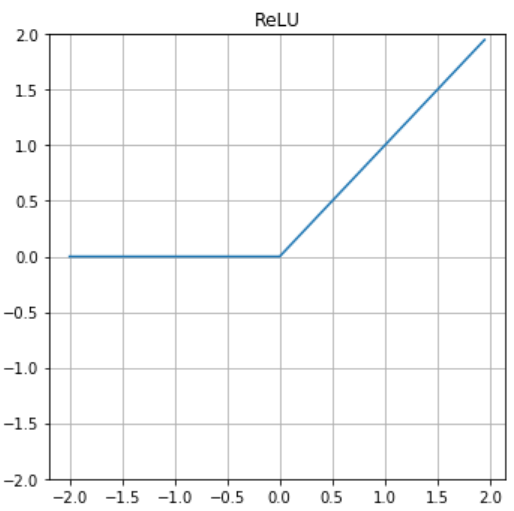
\includegraphics[width=.8\textwidth]{act_relu.png}
      \end{figure}


    \end{column}
  \end{columns}

  \begin{block}{Remarks}
    \begin{itemize}
    \item[+] Usable gradient when activated
    \item[+] Fast to compute
    \item[+] High abstraction
    \end{itemize}
  \end{block}

\pause

  \begin{alertblock}{}
    ReLU is the most commonly used activation function.
  \end{alertblock}


}

%%%%%%%%%%%%%%%%%%%%%%%%%%%%%%%%%%%%%%%%%%%%%%%%%%
\subsection{Artificial neuron as a classifier}
%%%%%%%%%%%%%%%%%%%%%%%%%%%%%%%%%%%%%%%%%%%%%%%%%%


%%%%%%%%%%%%%%%%%%%%%%%%%%%%%%%%%%%%%%%%%%%%%%%%%%

\frame{
\frametitle{What can an artificial neuron compute?}

\begin{figure}
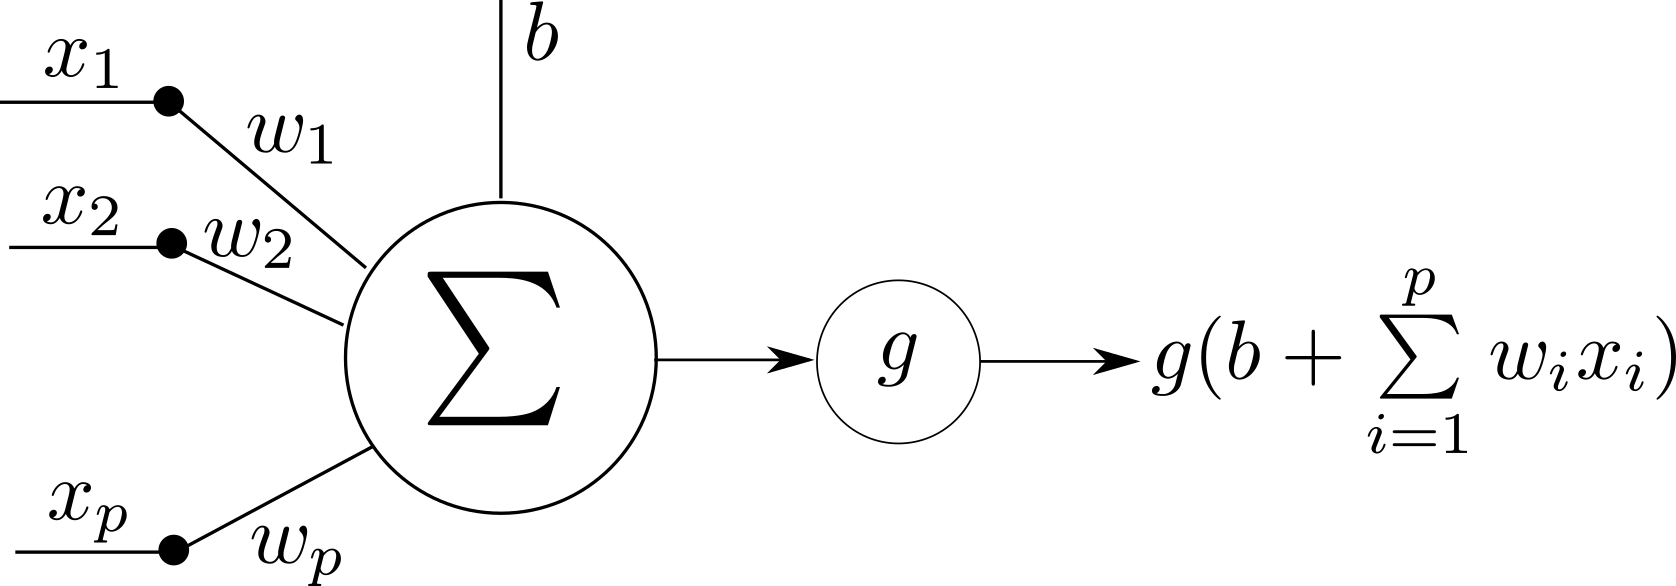
\includegraphics[height=3cm]{neurone}
\end{figure}

\begin{block}{}
  In $\R^p$ ,
  $b + \sum\limits_{i=0}^p w_ix_i = 0$
  corresponds to a hyperplane. For a given point
  $\x = \{x_0, \ldots, x_p\}$,
  decisions are made according to the side of the hyperplane it belongs to.
\end{block}

\begin{alertblock}{}
  When the activation function is binary, we obtain a \alert{perceptron}
\end{alertblock}

}

%%%%%%%%%%%%%%%%%%%%%%%%%%%%%%%%%%%%%%%%%%%%%%%%%%

\frame{
\frametitle{Example of what we can do with a neuron}

\begin{figure}
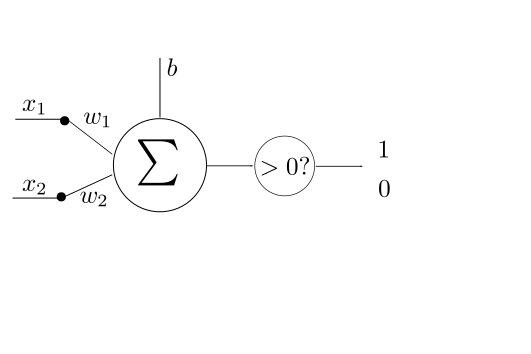
\includegraphics[height=3cm]{neurone_simple}
\end{figure}

\begin{itemize}
\item $p=2$ : 2-dimensional inputs (can be represented on a screen!)
\item Activation: binary
\item Classification problem
\end{itemize}
}

%%%%%%%%%%%%%%%%%%%%%%%%%%%%%%%%%%%%%%%%%%%%%%%%%%

\frame{
\frametitle{Gaussian clouds}

\begin{figure}
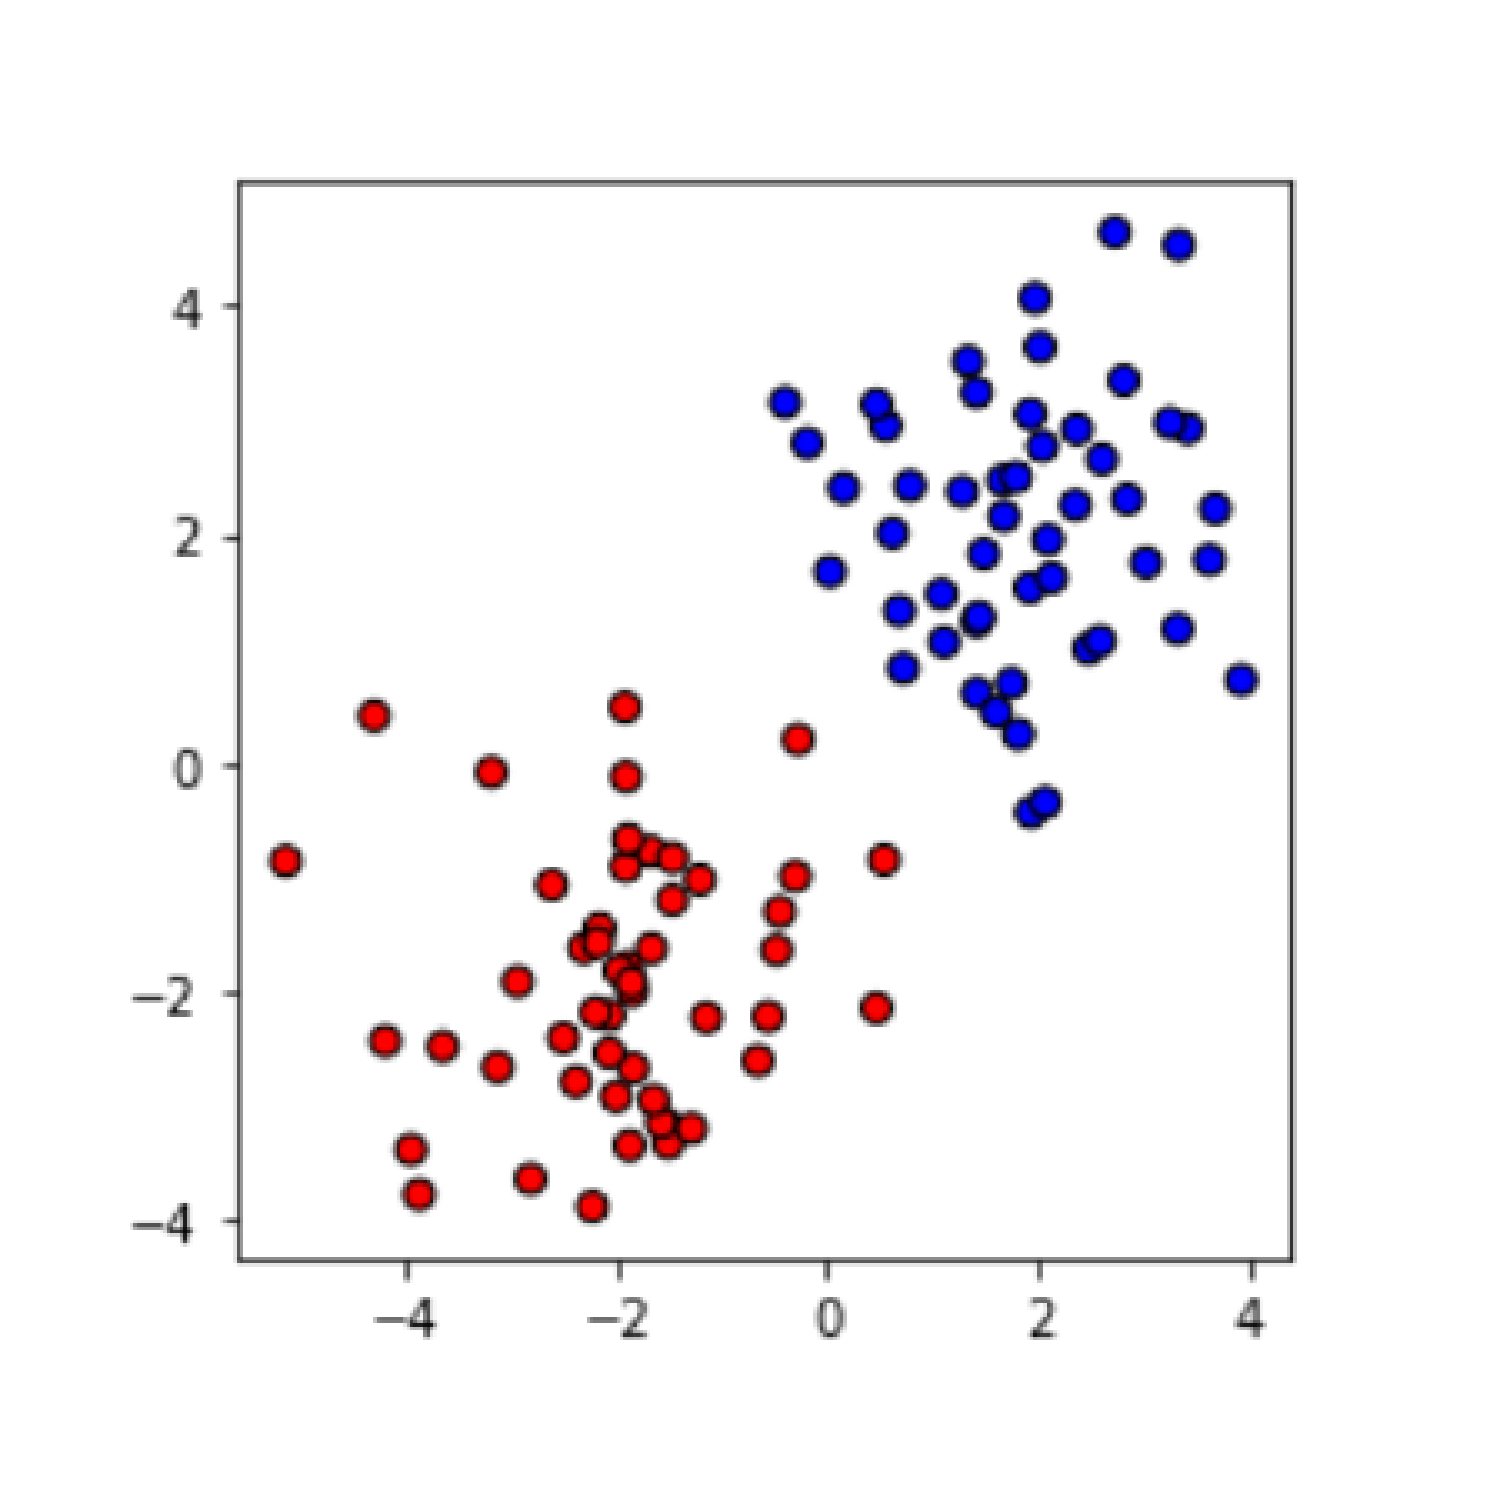
\includegraphics[height=6cm]{gaussian_clouds}
\end{figure}


}

%%%%%%%%%%%%%%%%%%%%%%%%%%%%%%%%%%%%%%%%%%%%%%%%%%

\frame{
\frametitle{Gaussian clouds}

\begin{figure}
\includegraphics[height=6cm]{gaussian_clouds_H}
\end{figure}


}

%%%%%%%%%%%%%%%%%%%%%%%%%%%%%%%%%%%%%%%%%%%%%%%%%%

\frame{
\frametitle{Circles}

\begin{figure}
\includegraphics[height=6cm]{circles}
\end{figure}


}

%%%%%%%%%%%%%%%%%%%%%%%%%%%%%%%%%%%%%%%%%%%%%%%%%%

\frame{
\frametitle{Circles}

\begin{figure}
\includegraphics[height=6cm]{circles_H}
\end{figure}

}

%%%%%%%%%%%%%%%%%%%%%%%%%%%%%%%%%%%%%%%%%%%%%%%%%%

\frame{
\frametitle{Solution}

\begin{columns}
  \begin{column}{.5\textwidth}
    \begin{figure}
      \includegraphics[height=5cm]{ann_5}
    \end{figure}

  \end{column}

  \begin{column}{.5\textwidth}

\begin{figure}
\includegraphics[height=4cm]{circles_H}
\end{figure}

  \end{column}
\end{columns}

}


%%%%%%%%%%%%%%%%%%%%%%%%%%%%%%%%%%%%
\begin{frame}{Artificial neuron compact representation}

    \begin{figure}
      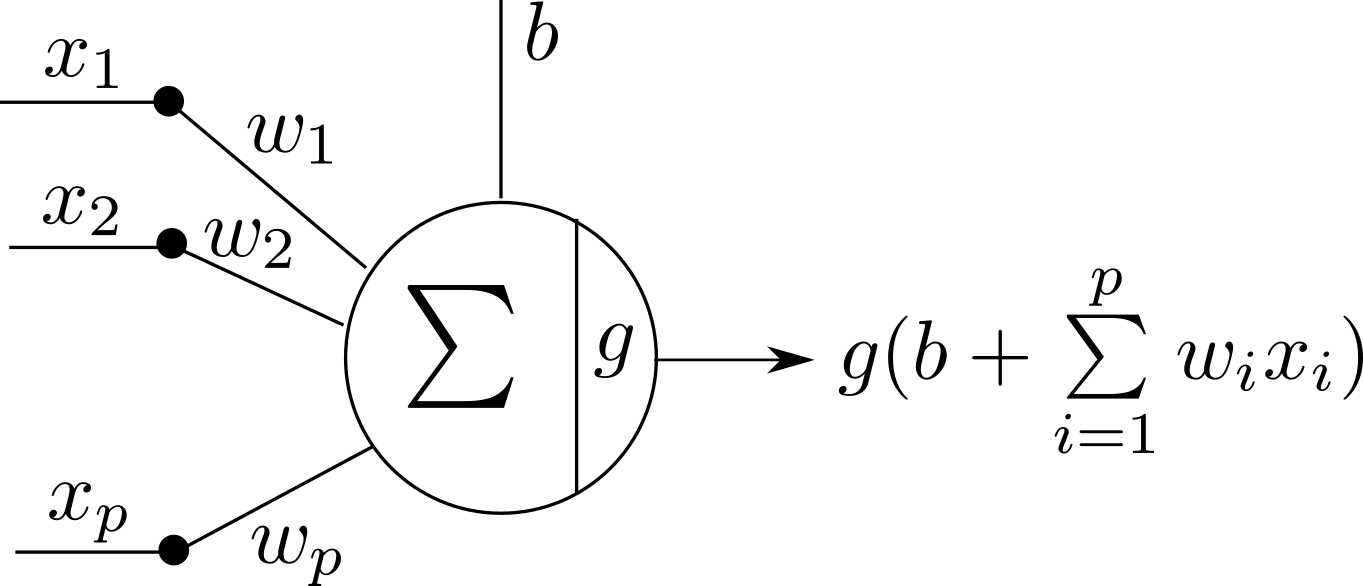
\includegraphics[height=3cm]{neurone_representation_compacte}
    \end{figure}

\end{frame}

%%%%%%%%%%%%%%%%%%%%%%%%%%%%%%%%%%%%%%%%%%%%%%%%%%
\section{Artificial neural networks}
%%%%%%%%%%%%%%%%%%%%%%%%%%%%%%%%%%%%%%%%%%%%%%%%%%

\subsection{Basic architectures}

%%%%%%%%%%%%%%%%%%%%%%%%%%%%%%%%%%%%%%%%%%%%%%
\frame{
\frametitle{Notations}

\begin{figure}
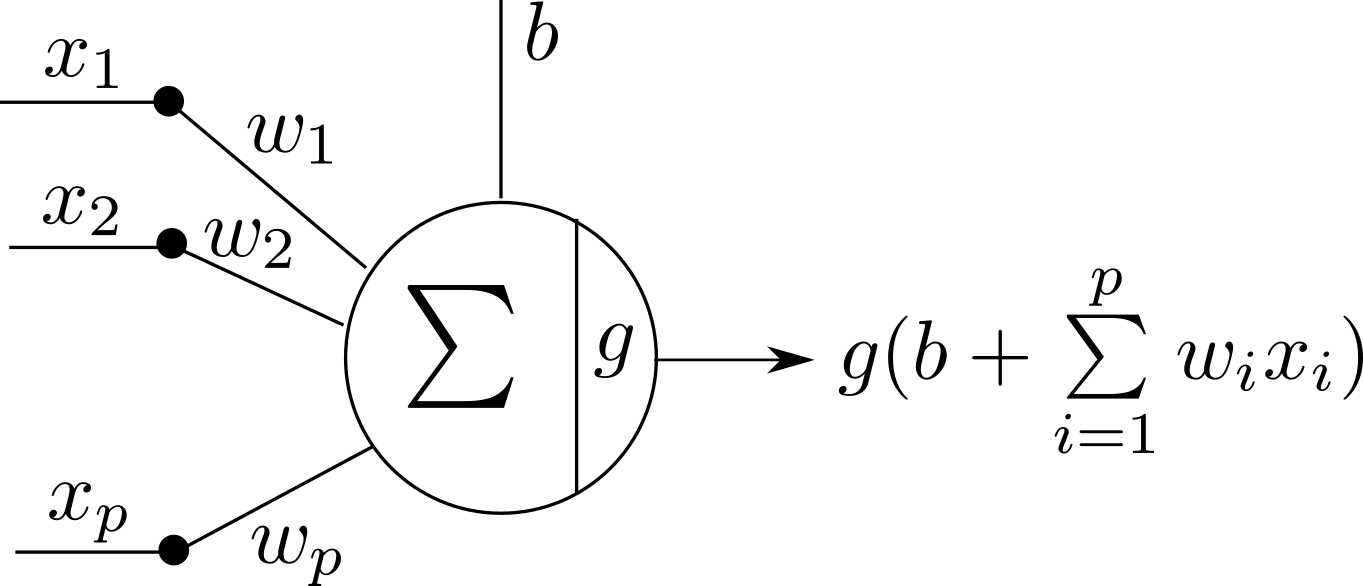
\includegraphics[height=3cm]{neurone_representation_compacte}
\end{figure}

  With
  \[
  \mathbf{w} = (w_1, \ldots, w_p)^T
  \]
  \[
  \x = (x_1, \ldots, x_p)^T
  \]

We can simply write:
\[
\act(b+ \sum\limits_{i=1}^p w_ix_i) = \act(b + \mathbf{w}^T\x)
\]

}

%%%%%%%%%%%%%%%%%%%%%%%%%%%%%%%%%%%%
\begin{frame}{Computation graph}

\begin{block}{Definition}
  A computation graph is a directly acyclic graph such that:
  \begin{itemize}
  \item A node is a mathematical operator
  \item To each edge is associated a value
  \item Each node can compute the values of its output edges from the values of its input edges
    \begin{itemize}
    \item Nodes without input edges are \emph{input nodes}. They represent the input values of the graph.
    \item Similarly, output values can be held in the \emph{output nodes}.
    \end{itemize}
  \end{itemize}
\end{block}

Computing a \emph{forward pass} through the graph means choosing its input values, and then progressively computing the values of all edges.


\end{frame}


%%%%%%%%%%%%%%%%%%%%%%%%%%%%%%%%%%%%
\begin{frame}{Computation graph example}
  We will compute:
  \[
  \sigma(w_1x + w_2y + b)
  \]
  where $\sigma$ is the sigmoid function: $\sigma(x) = \frac{1}{1 + e^{-x}}$

\vspace{3em}
\pause

  \centering
  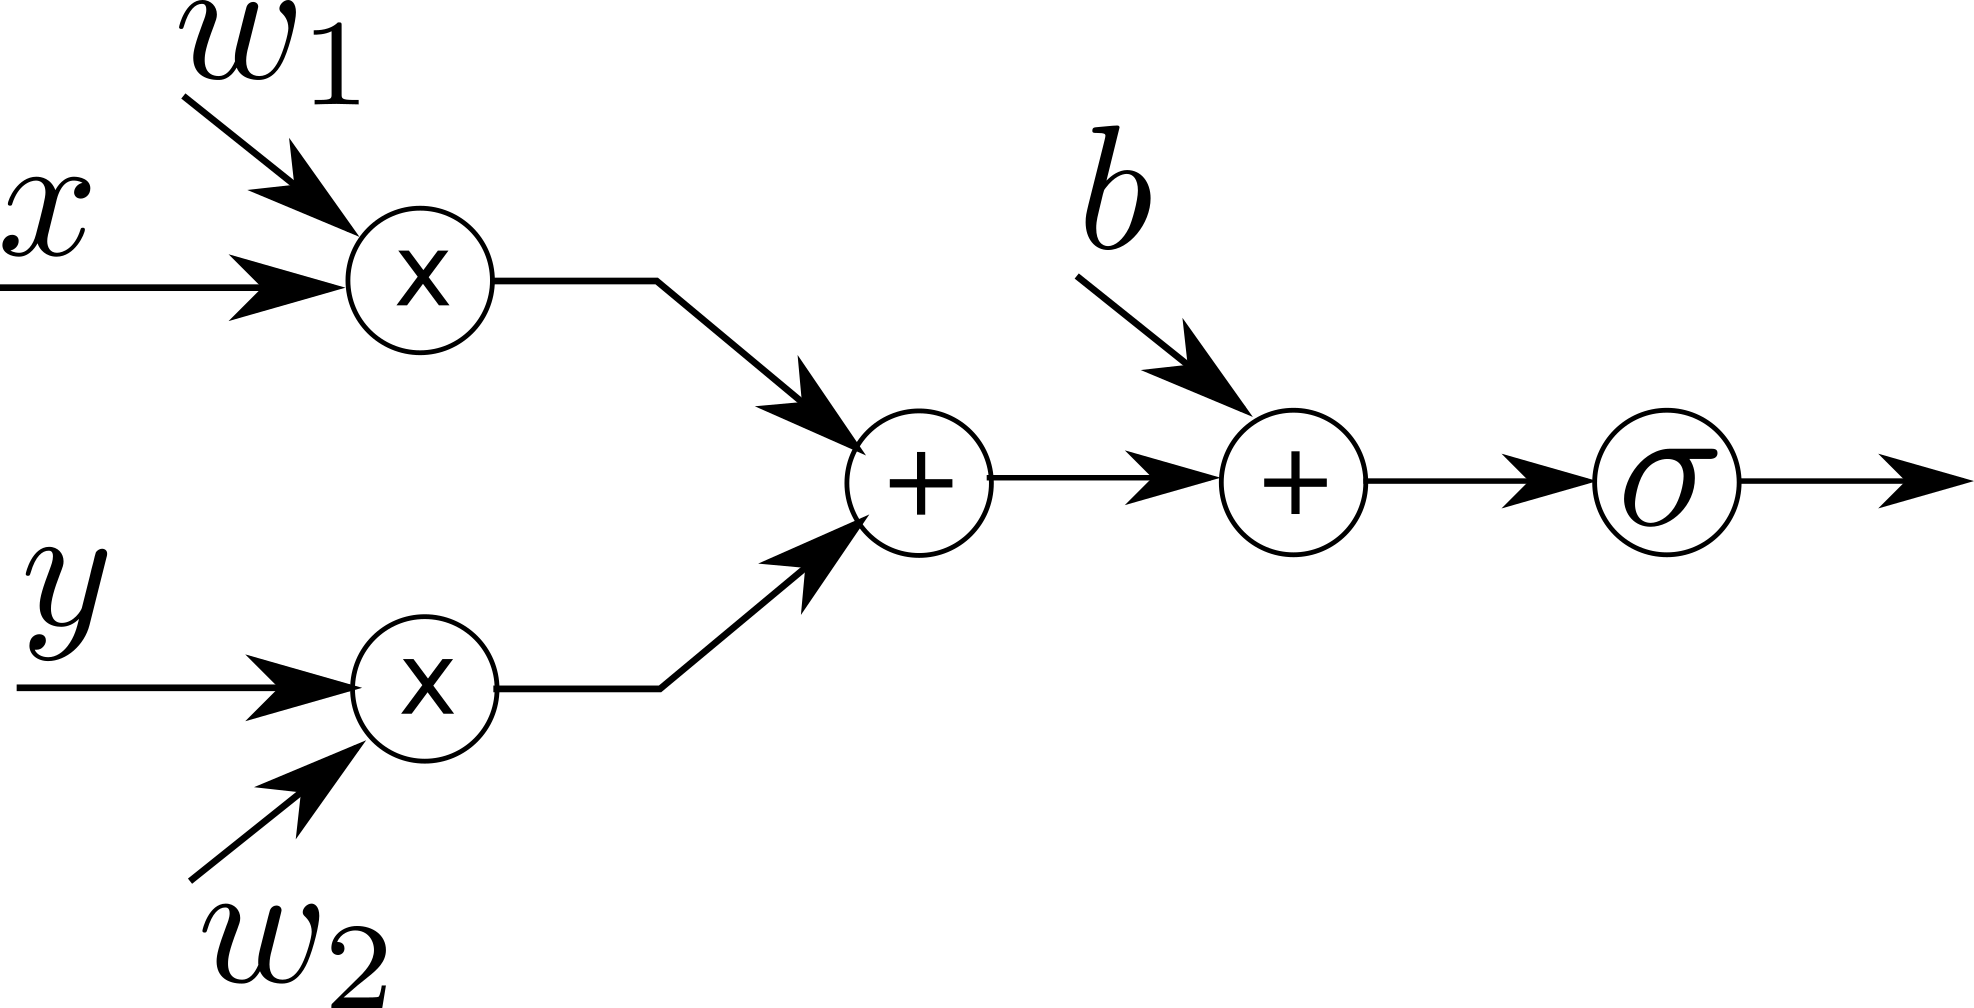
\includegraphics[width=0.6\textwidth]{compu_graph}


\end{frame}

%%%%%%%%%%%%%%%%%%%%%%%%%%%%%%%%%%%%%%%%%%%%%%%%%%
\frame{
\frametitle{Neural network (NN)}

\begin{block}{Definitions}
  \begin{itemize}
  \item An artificial neural network is a computation graph, where
   the nodes are artificial neurons
  \item The \alert{input layer} is the set of neurons without incoming edges.
  \item The \alert{output layer} is the set of neurons without outgoing edges.
  \end{itemize}

  \pause

  NB: Neural networks with cycles, know as recurrent neural networks, also exist.

\end{block}

}


%%%%%%%%%%%%%%%%%%%%%%%%%%%%%%%%%%%%%%%%%%%%%%%%%%
\frame{
\frametitle{Feed-forward neural networks}

\begin{block}{Definition}
  \begin{itemize}
  \item A feed-forward neural networks is a NN without cycles
  \item Neurons are organized in \alert{layers}
    \begin{itemize}
    \item A neuron belongs to layer $q$ if the longest path in the graph between the input layer and the neuron is of length $q$.
    \end{itemize}
  \item Any layers other than input and output layers are called \alert{hidden layers}
  \end{itemize}

\end{block}

\begin{figure}
  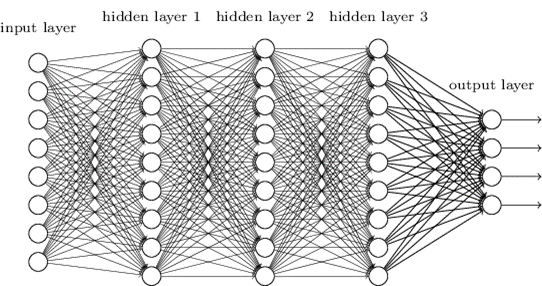
\includegraphics[height=3cm]{network.png}
\end{figure}

{\small(from http://www.jtoy.net)}

}

%%%%%%%%%%%%%%%%%%%%%%%%%%%%%%%%%%%%%%%%%%%%%%%%%%
\frame{
\frametitle{Feed-forward neural networks}

\begin{alertblock}{}
  In the following of this course, except when otherwise specified, all NNs will be feed-forward. Indeed, this is the preferred type of NN for image processing.
\end{alertblock}

\begin{block}{What about other architectures?}
  \begin{itemize}
    \item Recurrent neural networks (RNN)
    \item Long short-term memory networks (LSTM)
  \end{itemize}
\end{block}

\begin{itemize}
  \item[+] More powerful than feed-forward NNs
  \item[-] Complex dynamics; more difficult to train
  \item Mainly used for processing temporal data
\end{itemize}
}

%%%%%%%%%%%%%%%%%%%%%%%%%%%%%%%%%%%%%%%%%%%%%%%%%%
\frame{
\frametitle{Fully-connected network}

\begin{itemize}
\item A layer is said to be fully-connected (FC) if each of its neurons is connected to all the neurons of the previous layer
  \item  If a FC layer contains $r$ neurons, and the previous layer $q$, then its weights are 2D dimensional array (a matrix) of size $q \times r$
\item A NN is said to be fully connected if all its hidden layers are fully connected
\end{itemize}

\begin{figure}
  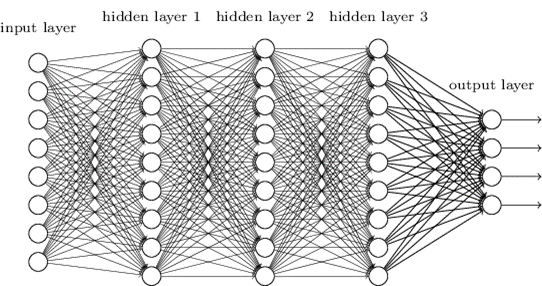
\includegraphics[height=3cm]{network.png}
\end{figure}

}


%%%%%%%%%%%%%%%%%%%%%%%%%%%%%%%%%%%%
\begin{frame}{Graphical representation of NNs}

\begin{columns}
  \begin{column}{.5\textwidth}
    \begin{figure}
      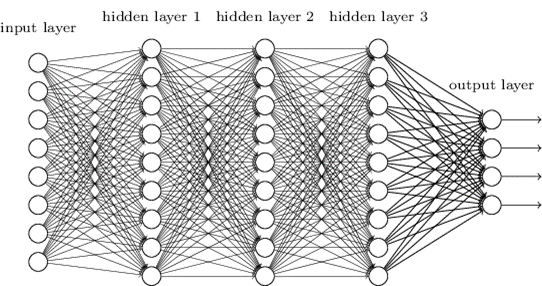
\includegraphics[height=3cm]{network.png}
    \end{figure}
    \begin{figure}
      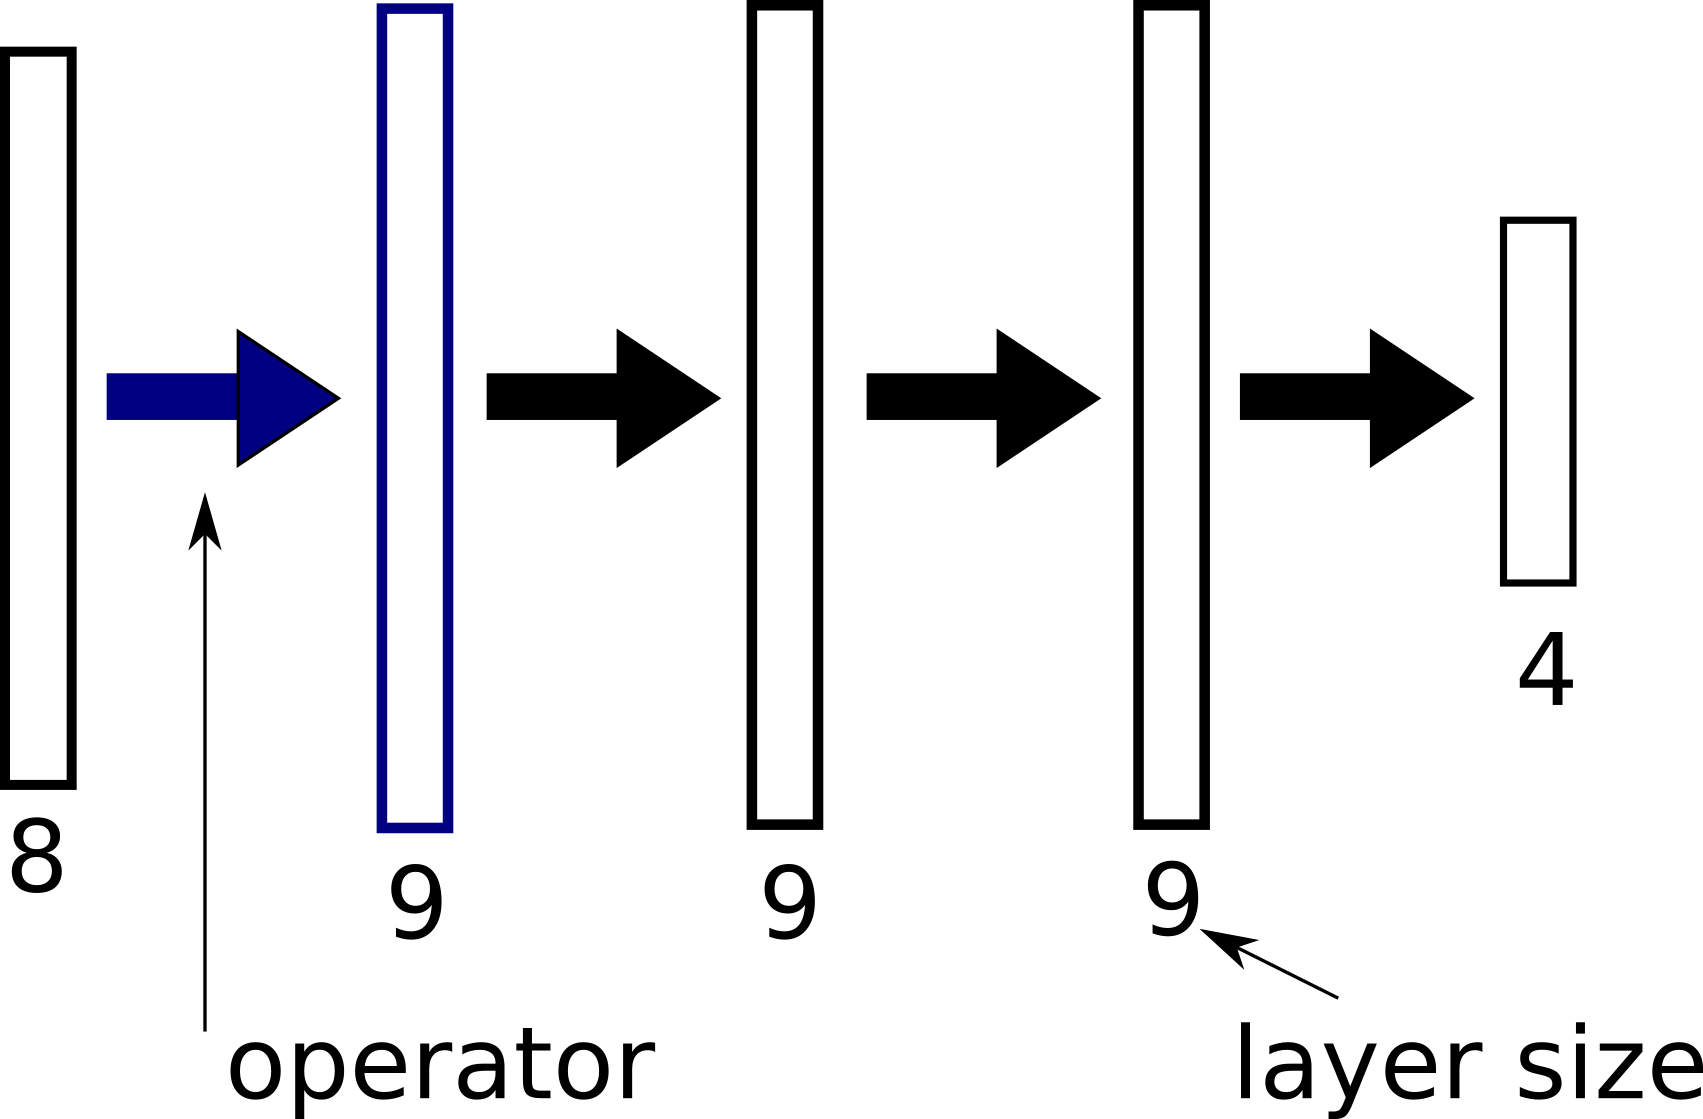
\includegraphics[height=3cm]{nn_representation}
    \end{figure}
  \end{column}

  \begin{column}{.5\textwidth}
    \begin{itemize}
    \item Data is organized into arrays, linked with operators
    \item A layer corresponds to an operator between arrays (and often an activation) as well as the resulting array.
    \end{itemize}
  \end{column}
\end{columns}


\end{frame}


%%%%%%%%%%%%%%%%%%%%%%%%%%%%%%%%%%%%
\begin{frame}{The equations of a fully connected neural network}

    \begin{figure}
      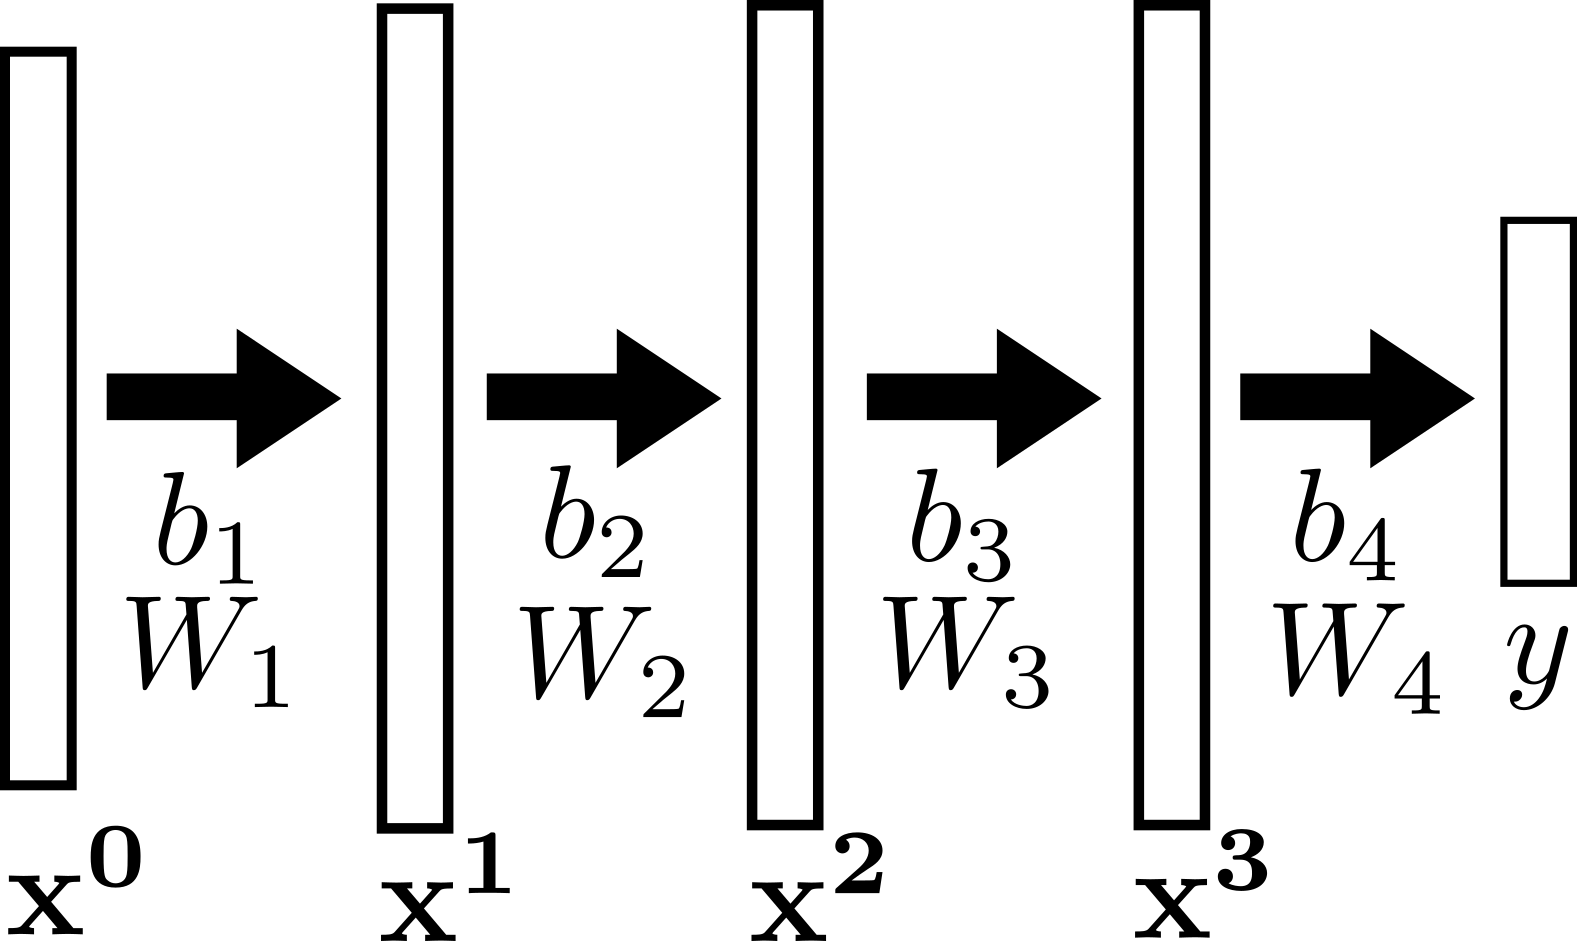
\includegraphics[height=3cm]{nn_representation2}
    \end{figure}

    \begin{block}{}
      \[\x^i = \act_i(\x^{i-1}\W_i + \bias_i),\, i= 1, 2, 3 \]
      \[y = \act_4(\x^4\W_4 + \bias_4)\]
    \end{block}

    \pause

    What would happen if all activation functions $\act_i$ were equal to the identity function?

\end{frame}

%%%%%%%%%%%%%%%%%%%%%%%%%%%%%%%%%%%%%%%%%%%%%%%%%%
\frame{
  \frametitle{Number of parameters}

  \begin{figure}
    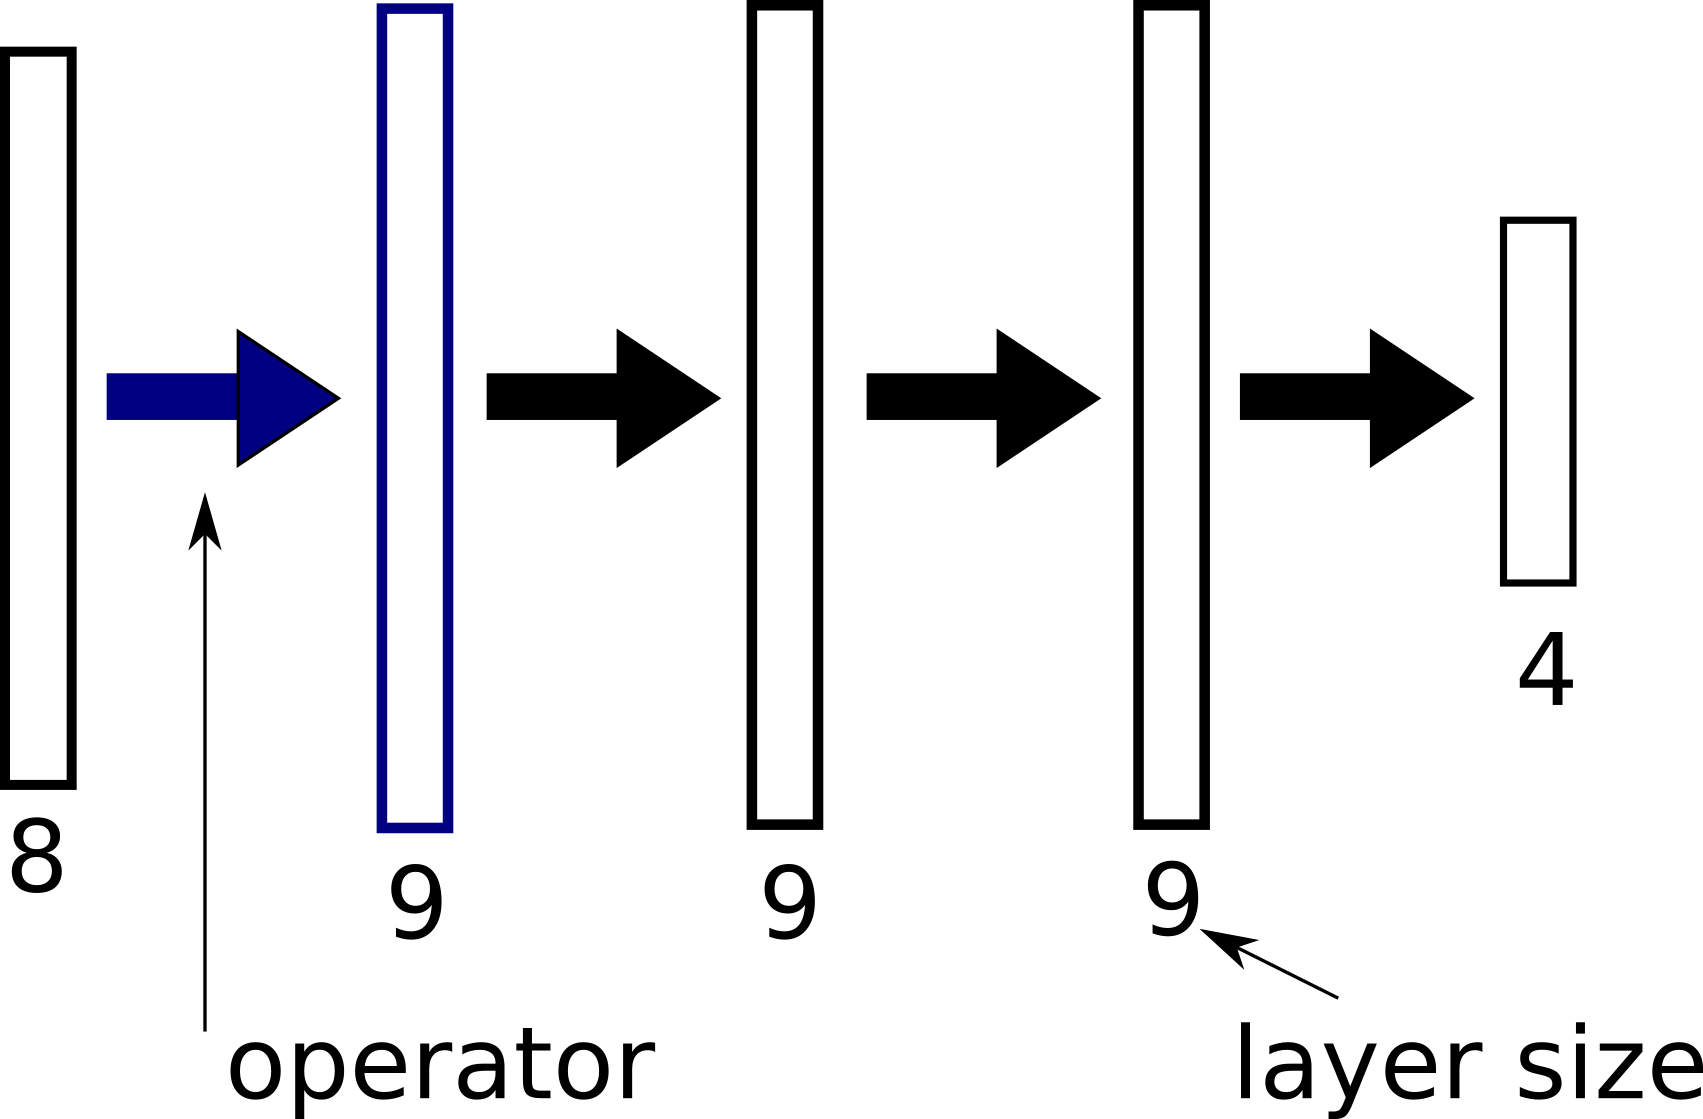
\includegraphics[height=3cm]{nn_representation.png}
  \end{figure}

  \begin{itemize}
  \item How many parameters does the above network contain?
  \item<2-> First hidden layer:\\
    %% \only<3->{$9$ neurons $\times 8$ neurons in the previous layer $+ 9$ biases $=81$}
    \begin{itemize}
    \item<3-> $9$ neurons $\times 8$ neurons in the previous layer $+ 9$ biases $=81$
    \end{itemize}
  \item<4-> Second and third layers: \only<5->{$9 \times 9 + 9 =90$}
  \item<6-> Output layer: \only<7->{$4 \times 9 + 4$}
  \item<8-> Total: $305$ parameters
  \end{itemize}

}

%%%%%%%%%%%%%%%%%%%%%%%%%%%%%%%%%%%%
\begin{frame}{Batch processing}

  In a training context, our learning set contains $n$ samples of vectors of length $p$, that can be grouped into a matrix $X$ of size $n \times p$. The $n$ corresponding outputs $y_i$ can also be grouped into a vector $\y$ of length $n$. The resulting equations are:

  \begin{block}{}
    \[\X^i = \act_i(\X^{i-1}\W_i + \bias_i),\, i= 1, 2, 3 \]
    \[\y = \act_4(\X^4\W_4 + \bias_4)\]
  \end{block}


\end{frame}

%%%%%%%%%%%%%%%%%%%%%%%%%%%%%%%%%%%%
\begin{frame}{Mini-batch processing}

  \begin{itemize}[<+->]
  \item   When dealing with large databases (large $n$ and sometimes large $p$) for practical reasons the network cannot process the whole set in a single pass.
  \item   One can also separate the training databases into subsets containing $m$ samples ($m < n$), called \emph{mini-batches}.
\end{itemize}


\end{frame}

%%%%%%%%%%%%%%%%%%%%%%%%%%%%%%%%%%%%%%%%%%%%%%%%%%
\subsection{The power of neural networks}


%%%%%%%%%%%%%%%%%%%%%%%%%%%%%%%%%%%%%%%%%%%%%%%%%%
\frame{
\frametitle{Universal approximation theorem}

\begin{columns}
  \begin{column}{.5\textwidth}
    \begin{itemize}
    \item We have previously seen that a neuron can be used as a linear classifier and that combining several of them one can build complex classifiers
    \item We will see that this observation can be generalized
    \end{itemize}
  \end{column}

  \begin{column}{.5\textwidth}
    \begin{figure}
      \includegraphics[height=4cm]{circles_H}
    \end{figure}
  \end{column}
\end{columns}


}

%%%%%%%%%%%%%%%%%%%%%%%%%%%%%%%%%%%%%%%%%%%%%%%%%%
\frame{
\frametitle{Universal approximation theorem}

\begin{block}{}
  Let $f$ be a \textcolor{blue}{continuous} real-valued function of $[0,1]^p$ ($p \in \N^*$) and $\epsilon$ a strictly positive real. Let $\act$ be a non-constant, increasing, bounded real function (\emph{\small{the activation function}}).

  Then there exists an integer $q$, real vectors $\{\mathbf{w}_i\}_{1 \leq i \leq q}$ of $\R^p$, and reals $\{b_i\}_{1 \leq i \leq q}$ and $\{v_i\}_{1 \leq i \leq q}$ such that for all $\x$ in $[0,1]^p$:

  \[
   \left| f(\x) - \sum\limits_{i=1}^q v_i \act(\mathbf{w}_i^T\x + b_i) \right| < \epsilon
  \]

\end{block}

A first version of this theorem, using sigmoidal activation functions, was proposed by \cite{cybenko_approximations_1989}. The version above was demonstrated by \cite{hornik_approximation_1991}.

}

%%%%%%%%%%%%%%%%%%%%%%%%%%%%%%%%%%%%%%%%%%%%%%%%%%
\frame{
\frametitle{Universal approximation theorem: what does it mean?}

  \[
   \left| f(\x) - \sum\limits_{i=1}^q v_i \act(\mathbf{w}_i^T\x + b_i) \right| < \epsilon
  \]

This means that function $f$ can be approximated with a neural network containing:
\begin{itemize}
  \item an input layer of size $p$;
  \item a hidden layer containing $q$ neurons with activation function $\act$, weights $\mathbf{w}_i$ and biases $b_i$;
  \item an output layer containing a single neuron, with weights $v_i$ (and an identity activation function).
\end{itemize}

}


%%%%%%%%%%%%%%%%%%%%%%%%%%%%%%%%%%%%%%%%%%%%%%%%%%
\frame{
  \frametitle{Universal approximation theorem in practice}

  \begin{itemize}
  \item The number of neurons increases very rapidly with the complexity of the function
  \item Empirical evidence has shown that multi-layer architectures give better results
  \end{itemize}

  \begin{block}<2->{}
    A NN can potentially have a lot of parameters. How can we set them?
\end{block}

}



%%%%%%%%%%%%%%%%%%%%%%%%%%%%%%%%%%%%%%%%%%%%%%%%%
\section{Training a neural network}
%%%%%%%%%%%%%%%%%%%%%%%%%%%%%%%%%%%%%%%%%%%%%%%%%

%%%%%%%%%%%%%%%%%%%%%%%%%%%%%%%%%%%%%%%%%%%%%%%%%
\begin{frame}{Introduction}

\begin{itemize}
\item We have seen that NNs have a lot of potential. However, how can the parameters $\param = (\W_i, \bias_i)$  be set?
\item What is our objective ?
\item A very general solution, that is also the mostly used, is \alert{gradient descent}
\end{itemize}

\end{frame}


%%%%%%%%%%%%%%%%%%%%%%%%%%%%%%%%%%%%
\begin{frame}{Learning problem}

  We recall that our training set contains $n$ samples:

  \[
  (\x_i, y_i) \in \R^p \times \R
  \]

  We \textcolor{blue}{choose} a family $f_{\param}$
  of functions from $\R^p$ into $\R$,
  depending on our set of parameters $\param$,
  and \textcolor{blue}{find} the value of $\param$
  that minimizes a \textcolor{blue}{chosen} loss function $\loss$:

\[
\param ^{\ast} = \argmin_{\param} ( \loss (\param) + \mathcal{R}(\param) )
\]

where $\mathcal{R}(\param)$ is a regularization term.

\vspace{1em}

\small{For the time being, for the sake of simplicity, we will drop the regularization term until further notice}

\end{frame}

%%%%%%%%%%%%%%%%%%%%%%%%%%%%%%%%%%%%
\begin{frame}{Loss function}

  A general form of the loss function is:
  \[
  \loss(\param) = \sum\limits_{i=1}^n d(y_i, f(\x_i, \param))
  \]
  where $d$ is some disparity function (the more similar its parameters, the smaller its value).

\end{frame}


%%%%%%%%%%%%%%%%%%%%%%%%%%%%%%%%%%%%
\begin{frame}{Loss function: examples}


  \begin{block}{Squared error}
    \[
    \loss(\param) = \sum\limits_{i=1}^n (y_i - f(\x_i, \param))^2
    \]
    This loss function is mainly used in regression problems.
  \end{block}

  \begin{block}{Binary cross-entropy}
    In this case, $y_i \in \{0, 1\}$:
    \[
    \loss(\param) = -\sum\limits_{i=1}^n \Big(y_i \log( f(\x_i, \param)) + (1 - y_i) \log(1 - f(\x_i, \param))\Big)
    \]
    This loss function is used in binary classification problems, where the network's output can be interpreted as a probability of belonging to a class.
  \end{block}

\end{frame}


%%%%%%%%%%%%%%%%%%%%%%%%%%%%%%%%%%%%
\begin{frame}{Gradient descent}

\begin{block}{Definition}
  Gradient descent is an optimization algorithm. For a derivable function $\loss$, a positive real $\gamma$ (the \alert{learning rate}) and a starting point $\param_0$, it computes a sequence of values:
  \[
  \forall e \in \N: \param_{e+1} = \param_e - \gamma \nabla \loss(\param_e)
  \]
\end{block}

\begin{block}{Property}
  If $\gamma$ is small enough, then:
  \[
  \loss(\param_{i+1}) \leq \loss(\param_i)
  \]
\end{block}

Gradient descent is an essential tool in optimization.

\end{frame}

%%%%%%%%%%%%%%%%%%%%%%%%%%%%%%%%%%%%
\begin{frame}{Gradient descent in the scalar case}

\begin{columns}
  \begin{column}{.5\textwidth}
    \includegraphics[width=\textwidth]{gradient_descent}
  \end{column}

  \begin{column}{.5\textwidth}
    \[
    \param_{t+1} = \param_t - \gamma\nabla \loss(\param_t)
    \]
  \end{column}
\end{columns}

\end{frame}



%%%%%%%%%%%%%%%%%%%%%%%%%%%%%%%%%%%%
\begin{frame}{Gradient descent: stopping criteria}

  In practice:
  \[
  \forall e \in [0, \ldots, E-1]:\quad \param_{e+1} = \param_e - \gamma \nabla \loss(\param_e)
  \]

\begin{itemize}
\item Choose $E$ (the number of \alert{epochs}) based on experience
\item Track the quality of the model using a validation dataset and stop when the validation loss does not improve
\end{itemize}


\end{frame}
%%%%%%%%%%%%%%%%%%%%%%%%%%%%%%%%%%%%
\begin{frame}{Towards stochastic gradient descent}

  The loss function we initially defined depends on the whole training set:
  \[
  \loss(\param) = \sum\limits_{i=1}^n d(y_i, f(\x_i, \param))
  \]

\pause

  \begin{itemize}[<+->]
  \item If $n$ is very large, its computation is not feasible.
  \item A computation on the whole training set leads to a single update of the model parameters - convergence can therefore be slow.
  \end{itemize}

\end{frame}

%%%%%%%%%%%%%%%%%%%%%%%%%%%%%%%%%%%%
\begin{frame}{Stochastic gradient descent}

  In \alert{stochastic gradient descent}, the parameters are updated for each sample $i$.

\begin{itemize}[<+->]
\item
  First, the loss is computed

  \[
  \loss(\param_t) = d(y_i, f(\x_i, \param_t))
  \]
\item
  The gradient $\nabla \loss(\param_t)$ is computed through backpropagation and
\item Finally the parameters are updated:

  \[
    \param_{t+1} = \param_t - \gamma\nabla \loss(\param_t)
    \]
  \item
    Note that the learning rate $\gamma$ can have a different value than in straightforward gradient descent.
\end{itemize}




\end{frame}

%%%%%%%%%%%%%%%%%%%%%%%%%%%%%%%%%%%%
\begin{frame}{Gradient descent applied to neural networks}

  In the case of neural networks, the loss $\loss$ depends on each parameter $\param_i$ via the composition of several simple functions. In order to compute the gradient $\nabla_{\param}\loss$ we will make extensive use of the chain rule theorem.

  \begin{block}{Chain rule theorem}
    Let $f_1$ and $f_2$ be two derivable real functions ($\R \rightarrow \R$). Then for all $x$ in $\R$:   :
    \[
     (f_2 \circ f_1)'(x) = f_2'(f_1(x)).f_1'(x)
    \]
  \end{block}


\begin{block}{Leibniz notation}
  Let us introduce variables $x$, $y$ and $z$:
  \[x \xrightarrow{f_1} y \xrightarrow{f_2} z\]

  Then:
  \[\dv{z}{x} = \dv{z}{y} \cdot \dv{y}{x} \]

\end{block}

\end{frame}


%%%%%%%%%%%%%%%%%%%%%%%%%%%%%%%%%%%%
\begin{frame}{The backpropagation algorithm}

  \begin{itemize}
  \item The backpropagation algorithm is used in a neural network to efficiently compute the partial derivatives of the loss with respect to each parameter of the network.
  \item One can trace the origins of the method to the sixties
  \item It was first applied to NN in the eighties \cite{werbos_applications_1982, lecun_procedure_1985}
  \end{itemize}


\end{frame}



%%%%%%%%%%%%%%%%%%%%%%%%%%%%%%%%%%%%
\begin{frame}<handout>{Simple backpropagation example}

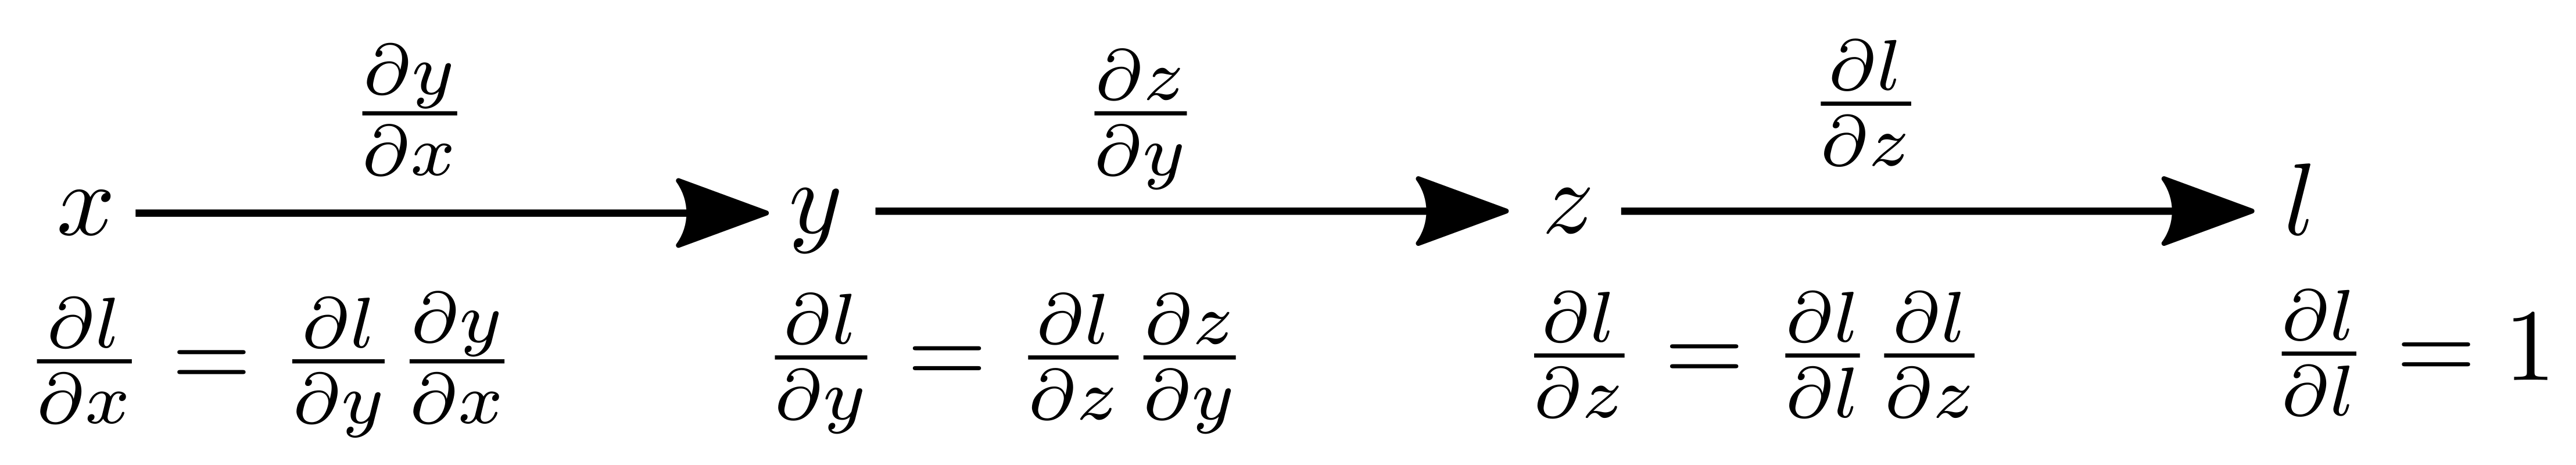
\includegraphics[width=\textwidth]{bp_simple.png}

\end{frame}

%%%%%%%%%%%%%%%%%%%%%%%%%%%%%%%%%%%%
\begin{frame}<beamer>{Simple backpropagation example}

\only<1>{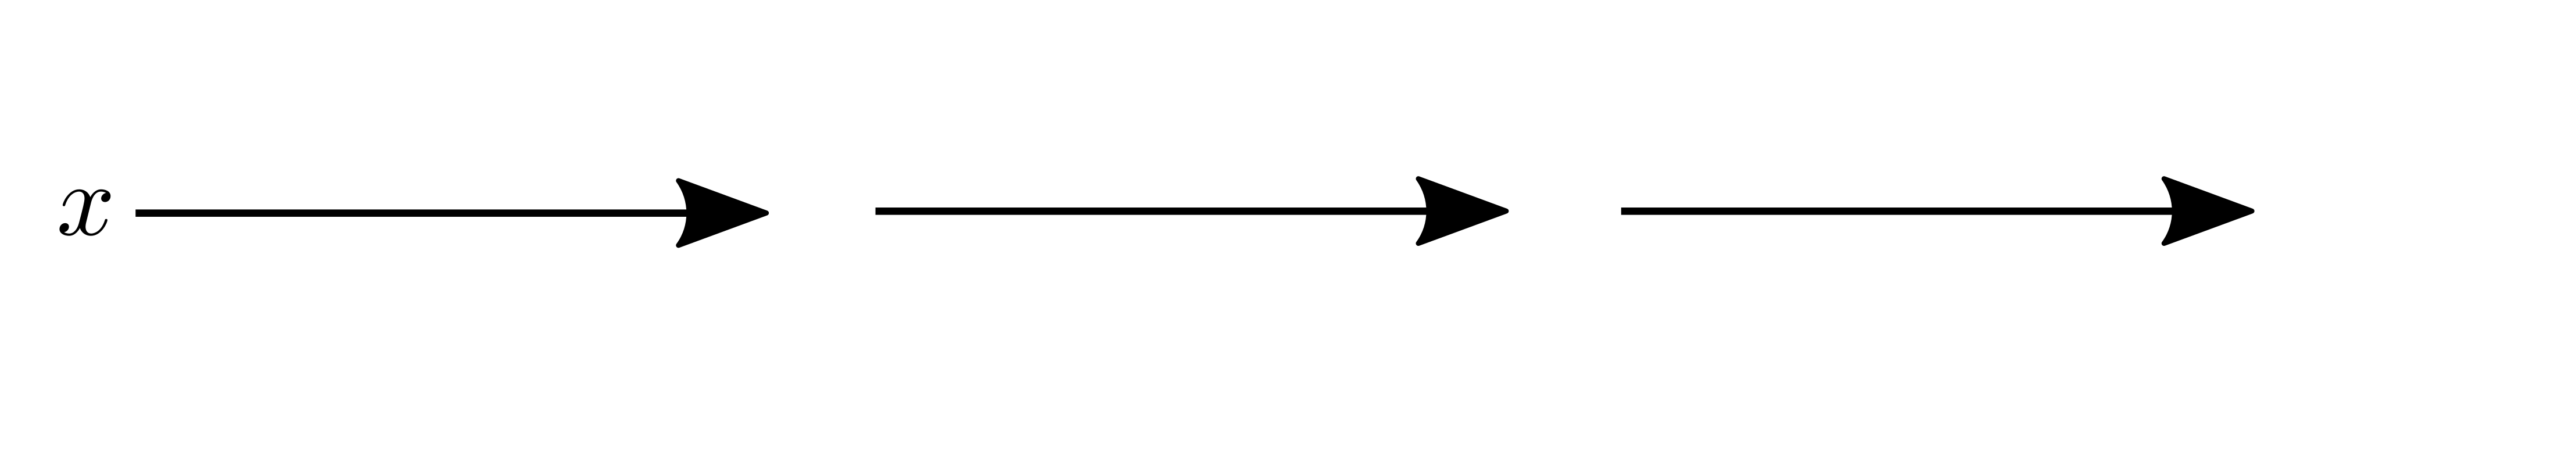
\includegraphics[width=\textwidth]{bp_simple_1.png}}
\only<2>{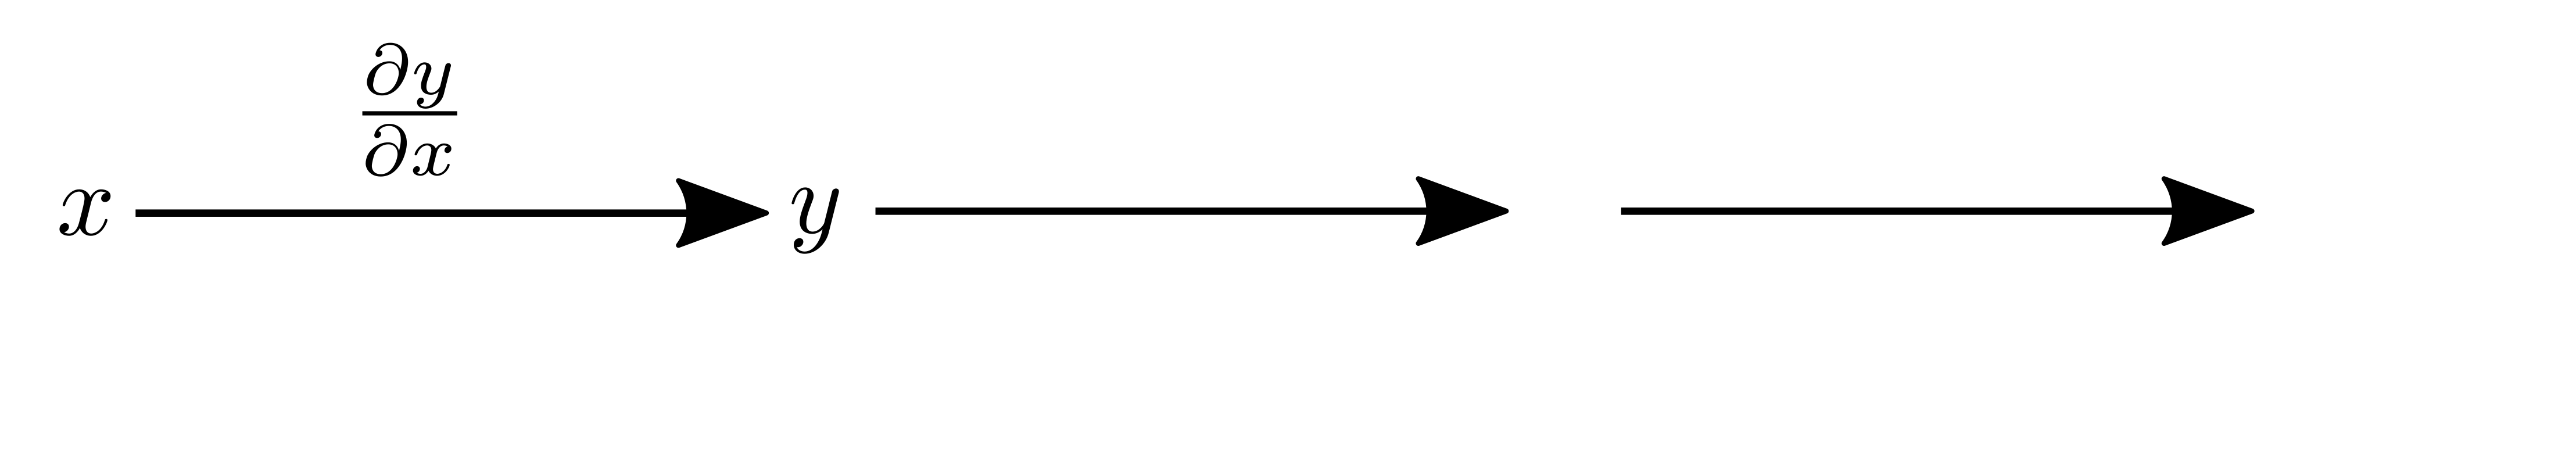
\includegraphics[width=\textwidth]{bp_simple_2.png}}
\only<3>{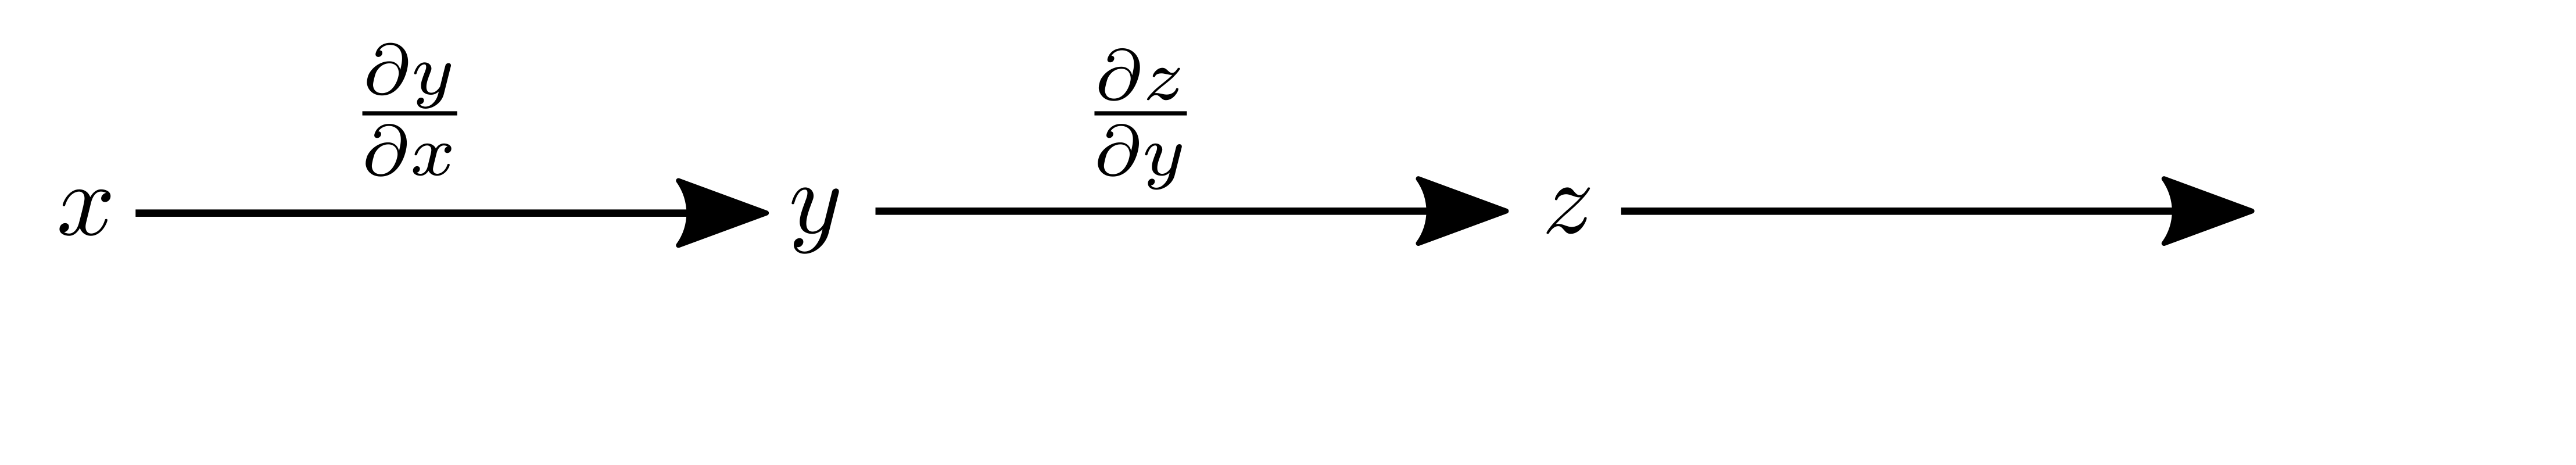
\includegraphics[width=\textwidth]{bp_simple_3.png}}
\only<4>{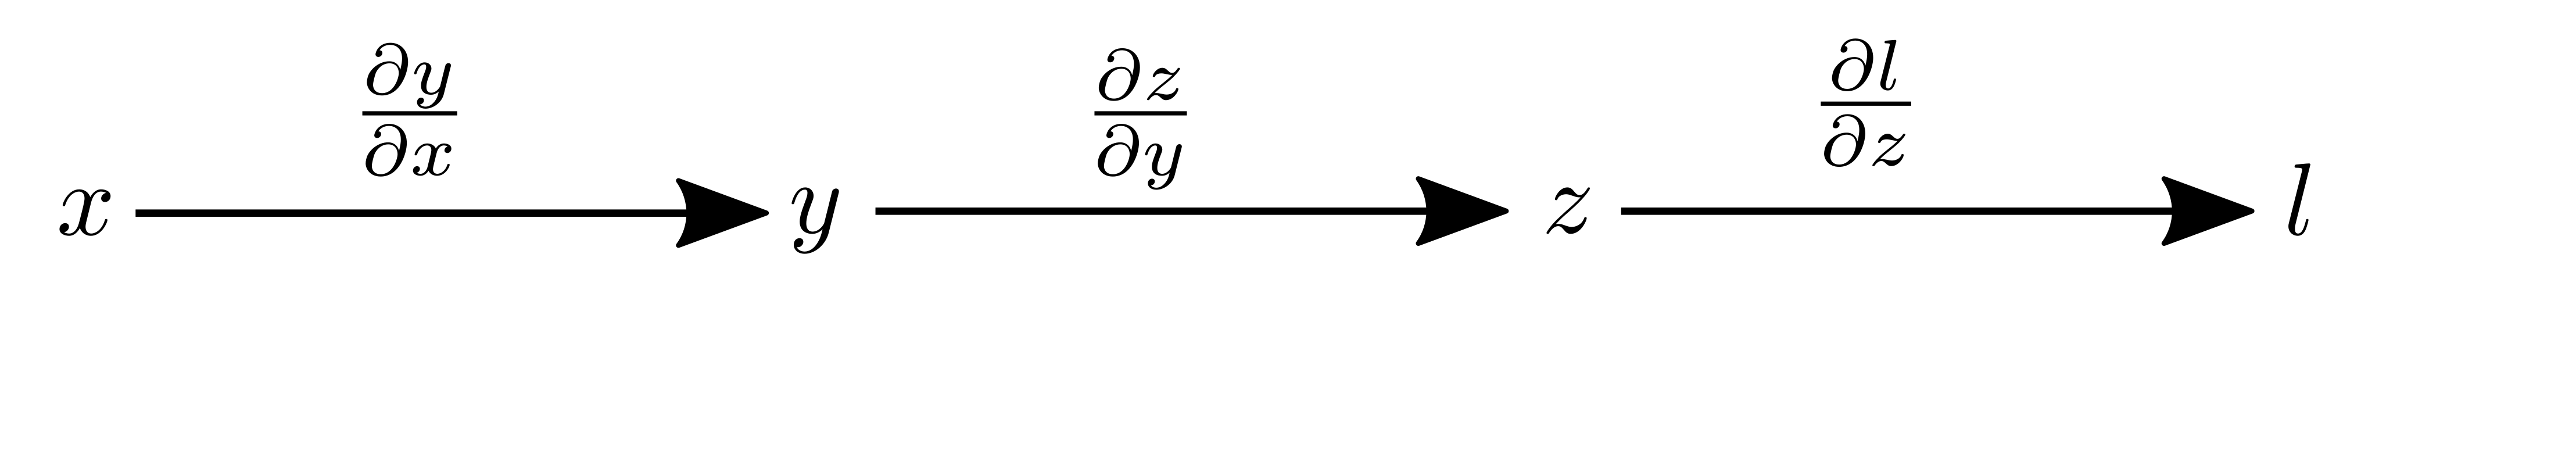
\includegraphics[width=\textwidth]{bp_simple_4.png}}
\only<5>{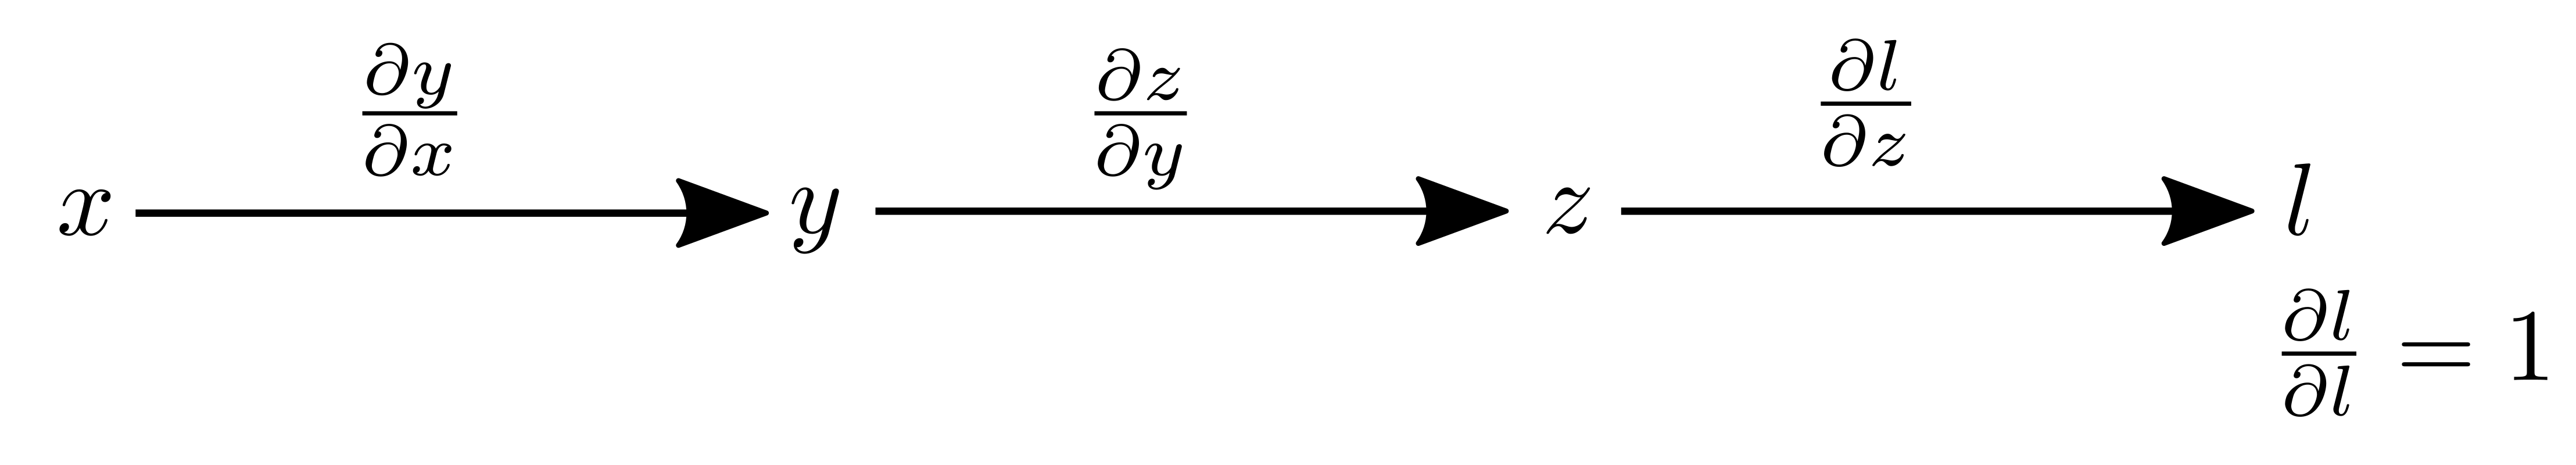
\includegraphics[width=\textwidth]{bp_simple_5.png}}
\only<6>{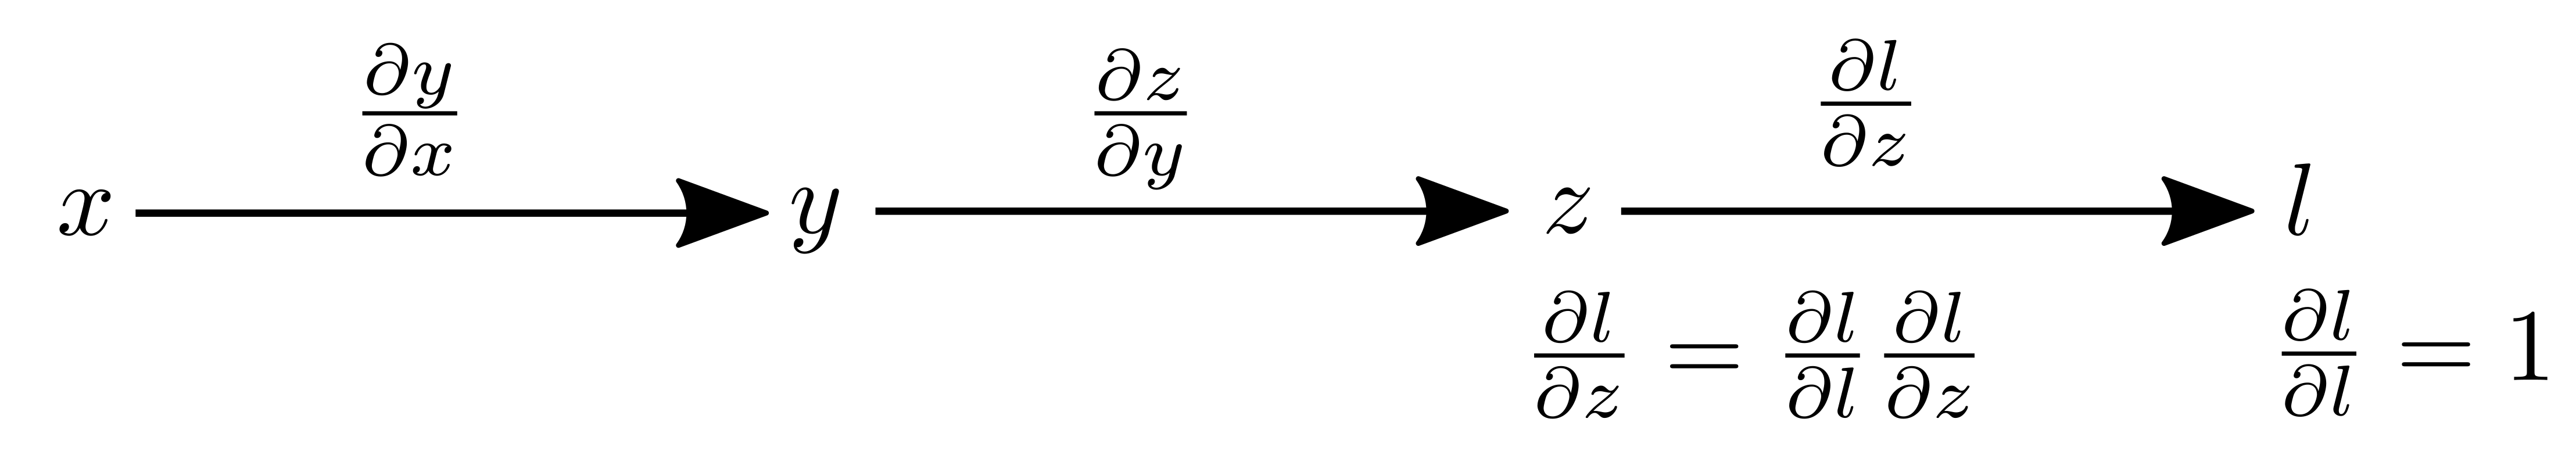
\includegraphics[width=\textwidth]{bp_simple_6.png}}
\only<7>{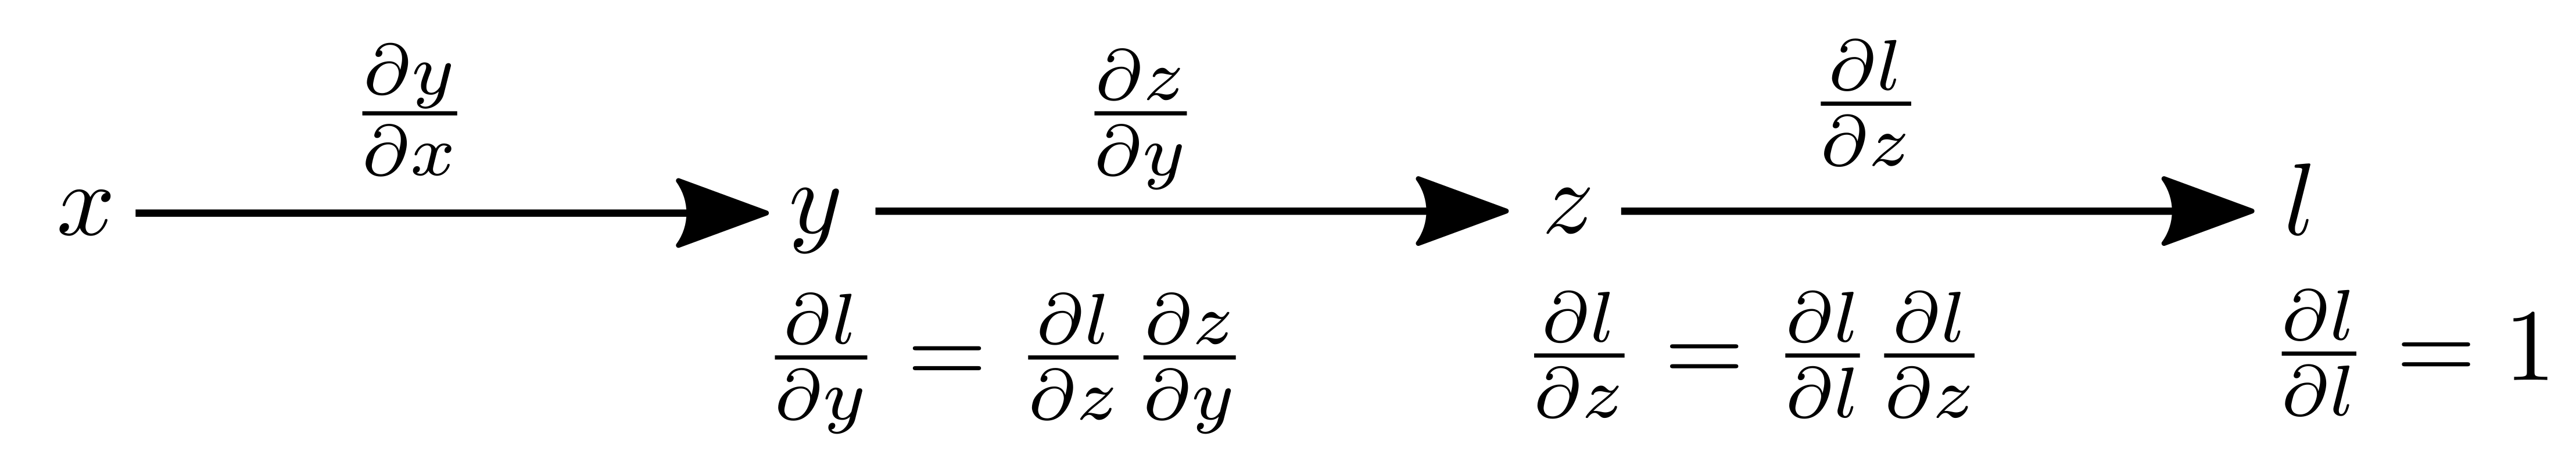
\includegraphics[width=\textwidth]{bp_simple_7.png}}
\only<8>{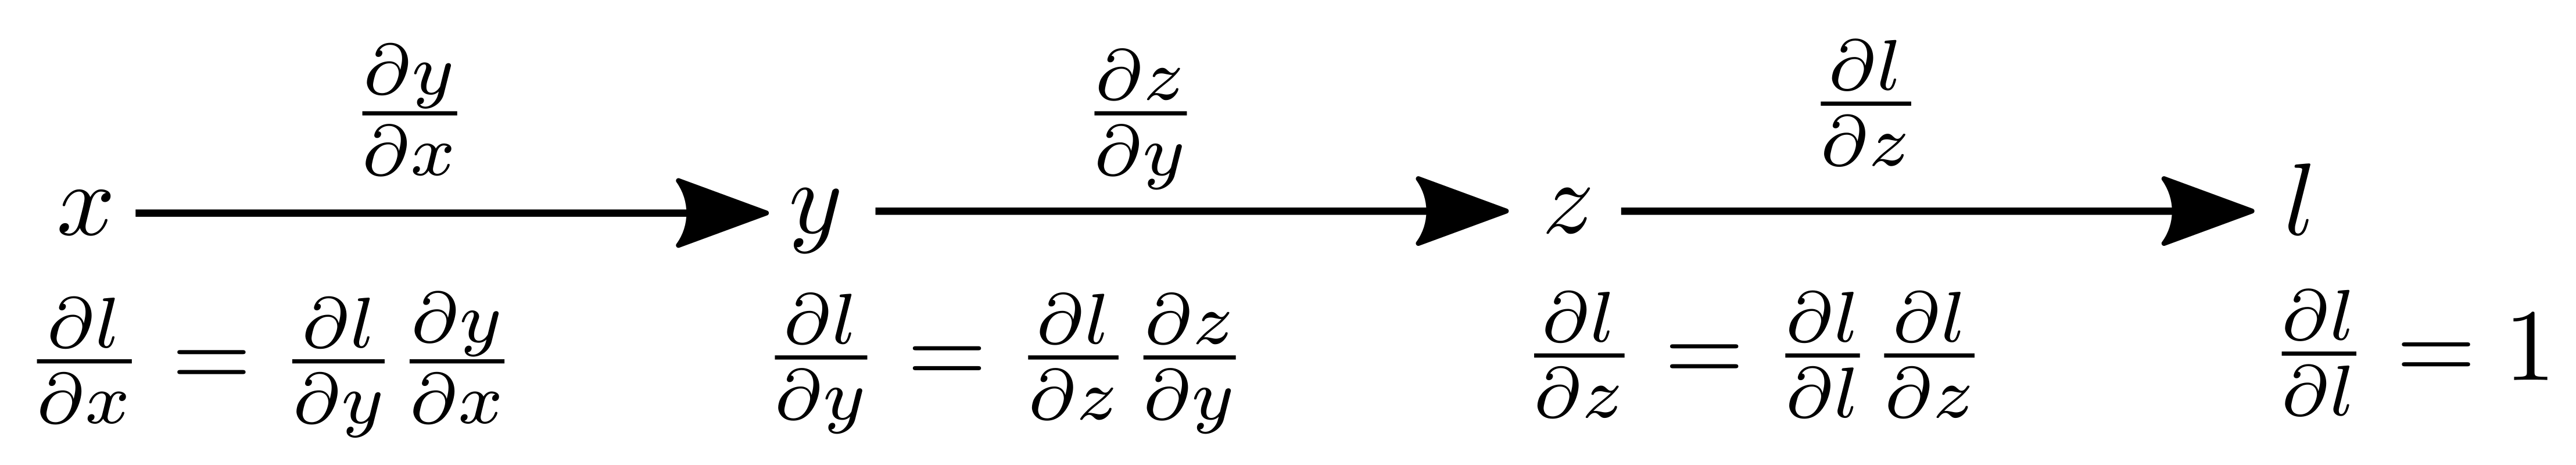
\includegraphics[width=\textwidth]{bp_simple_8.png}}

\end{frame}

%%%%%%%%%%%%%%%%%%%%%%%%%%%%%%%%%%%%
\begin{frame}<handout>{A more complex backpropagation example}

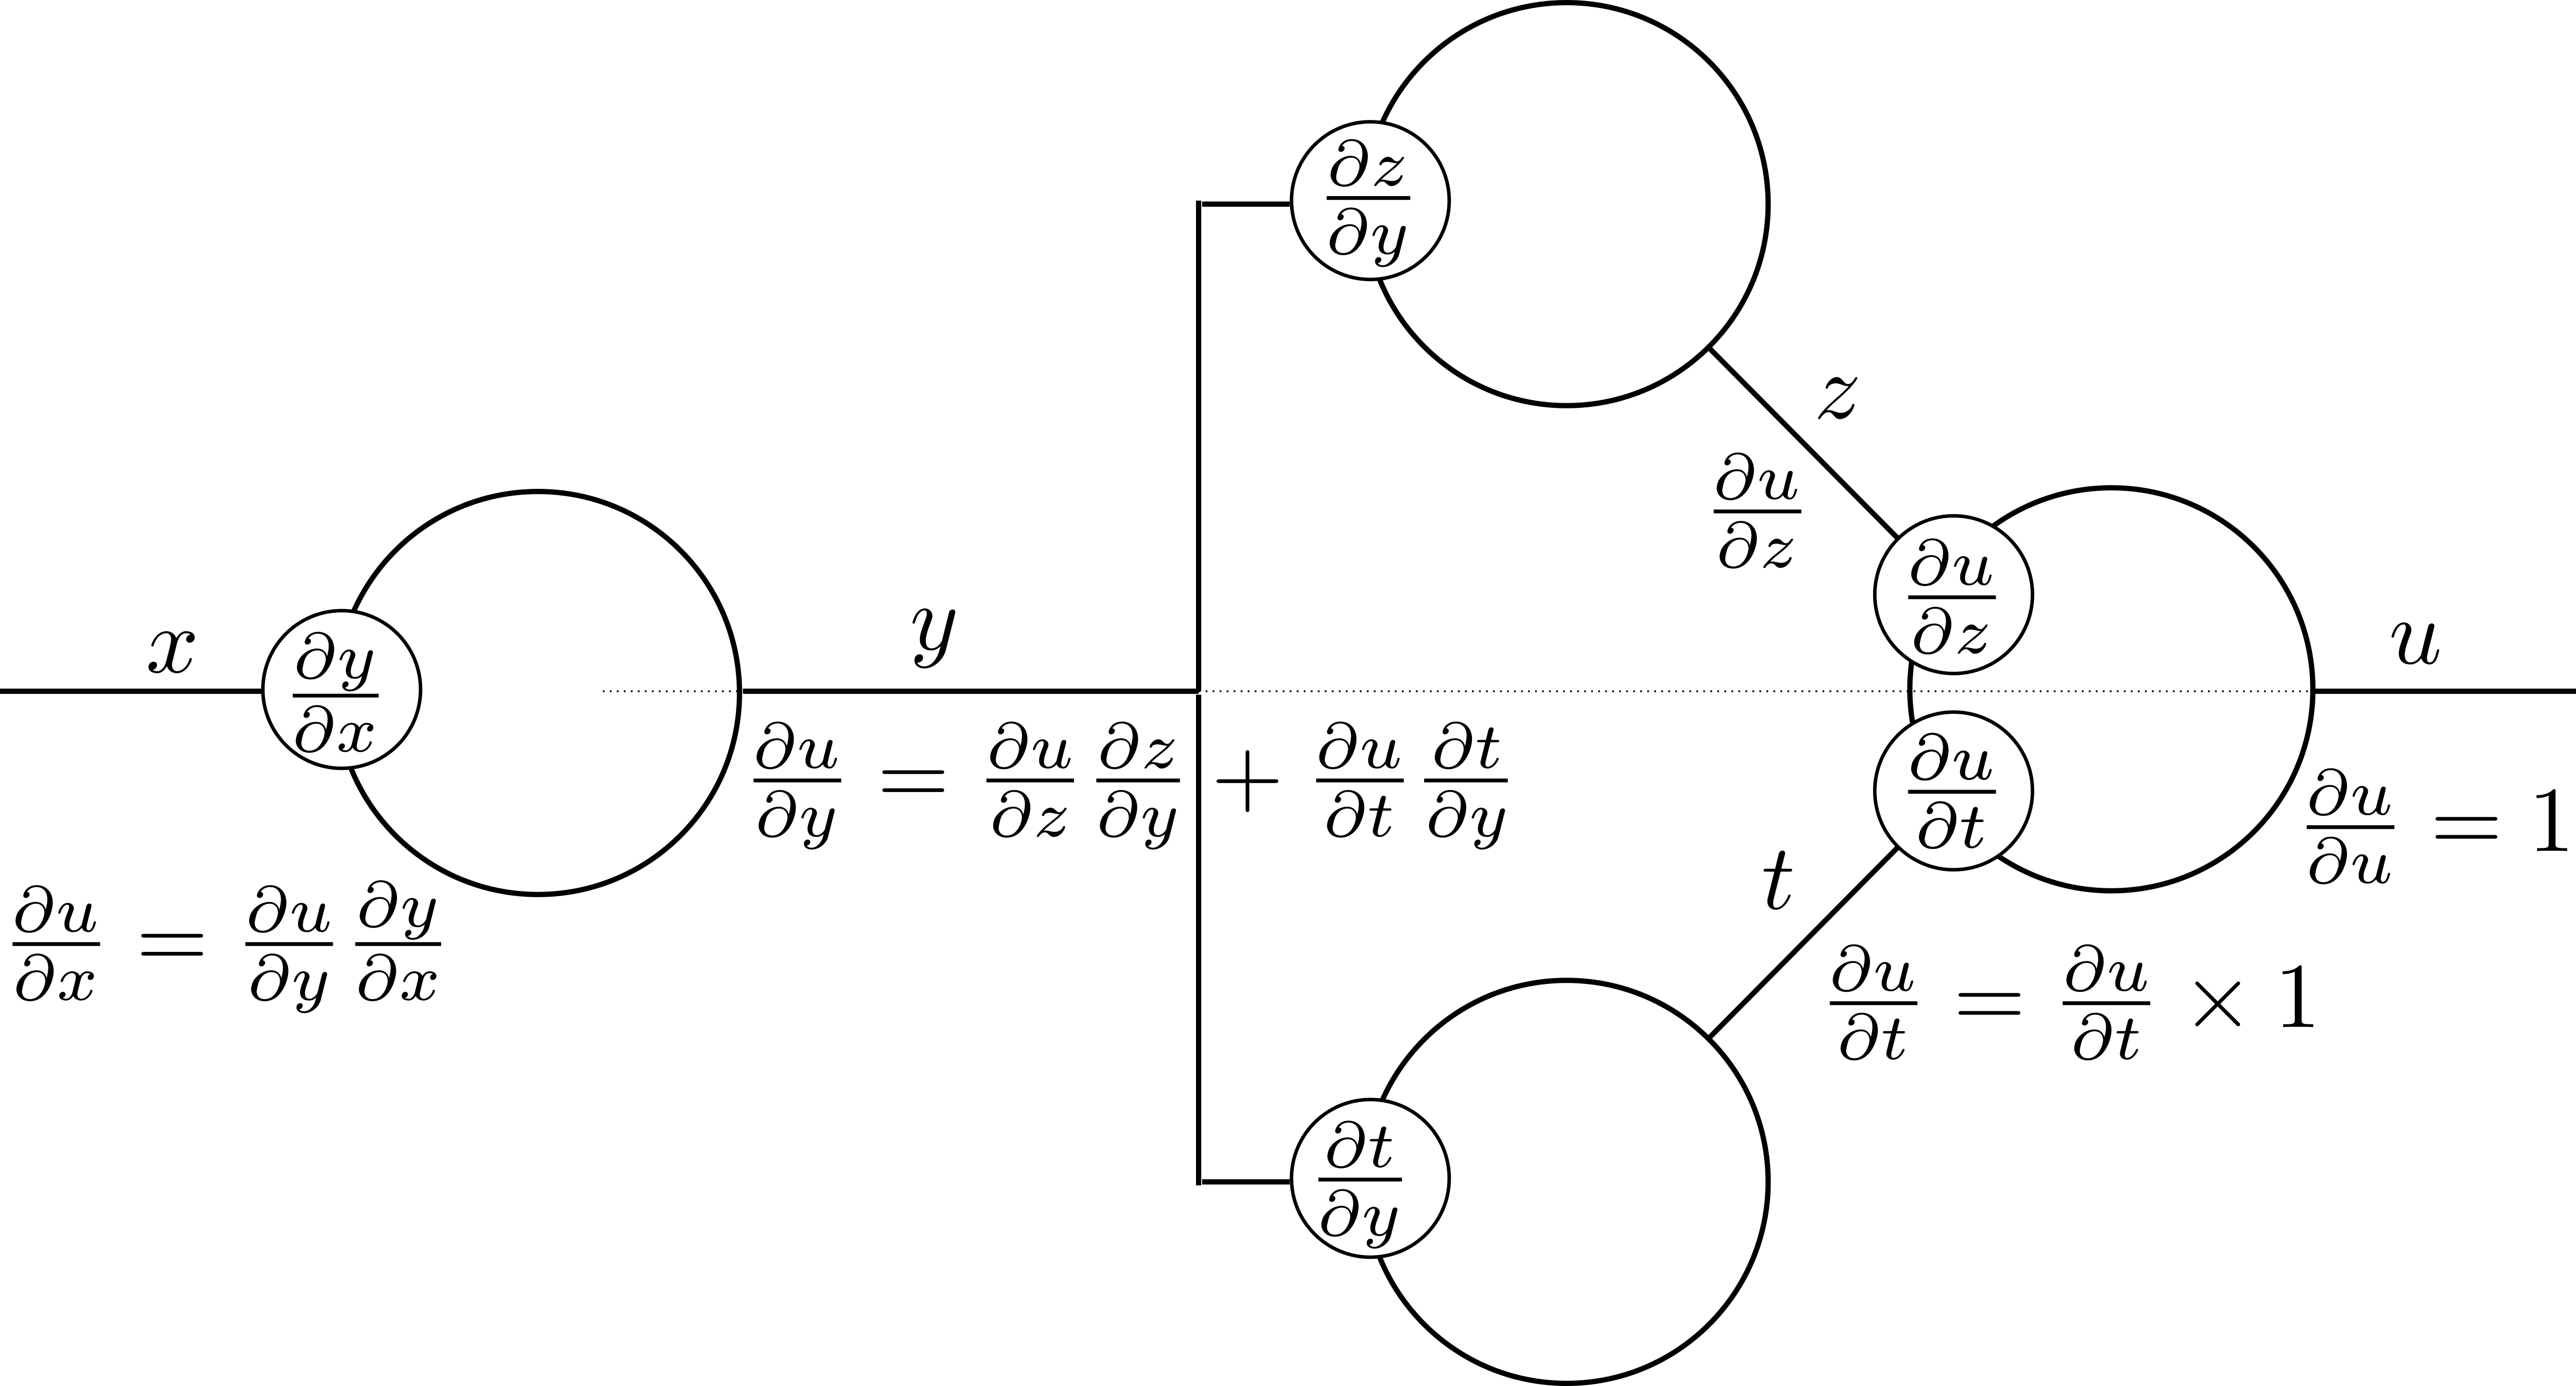
\includegraphics[width=\textwidth]{bp.png}

\end{frame}

%%%%%%%%%%%%%%%%%%%%%%%%%%%%%%%%%%%%
\begin{frame}<beamer>{Backpropagation example}

\only<1>{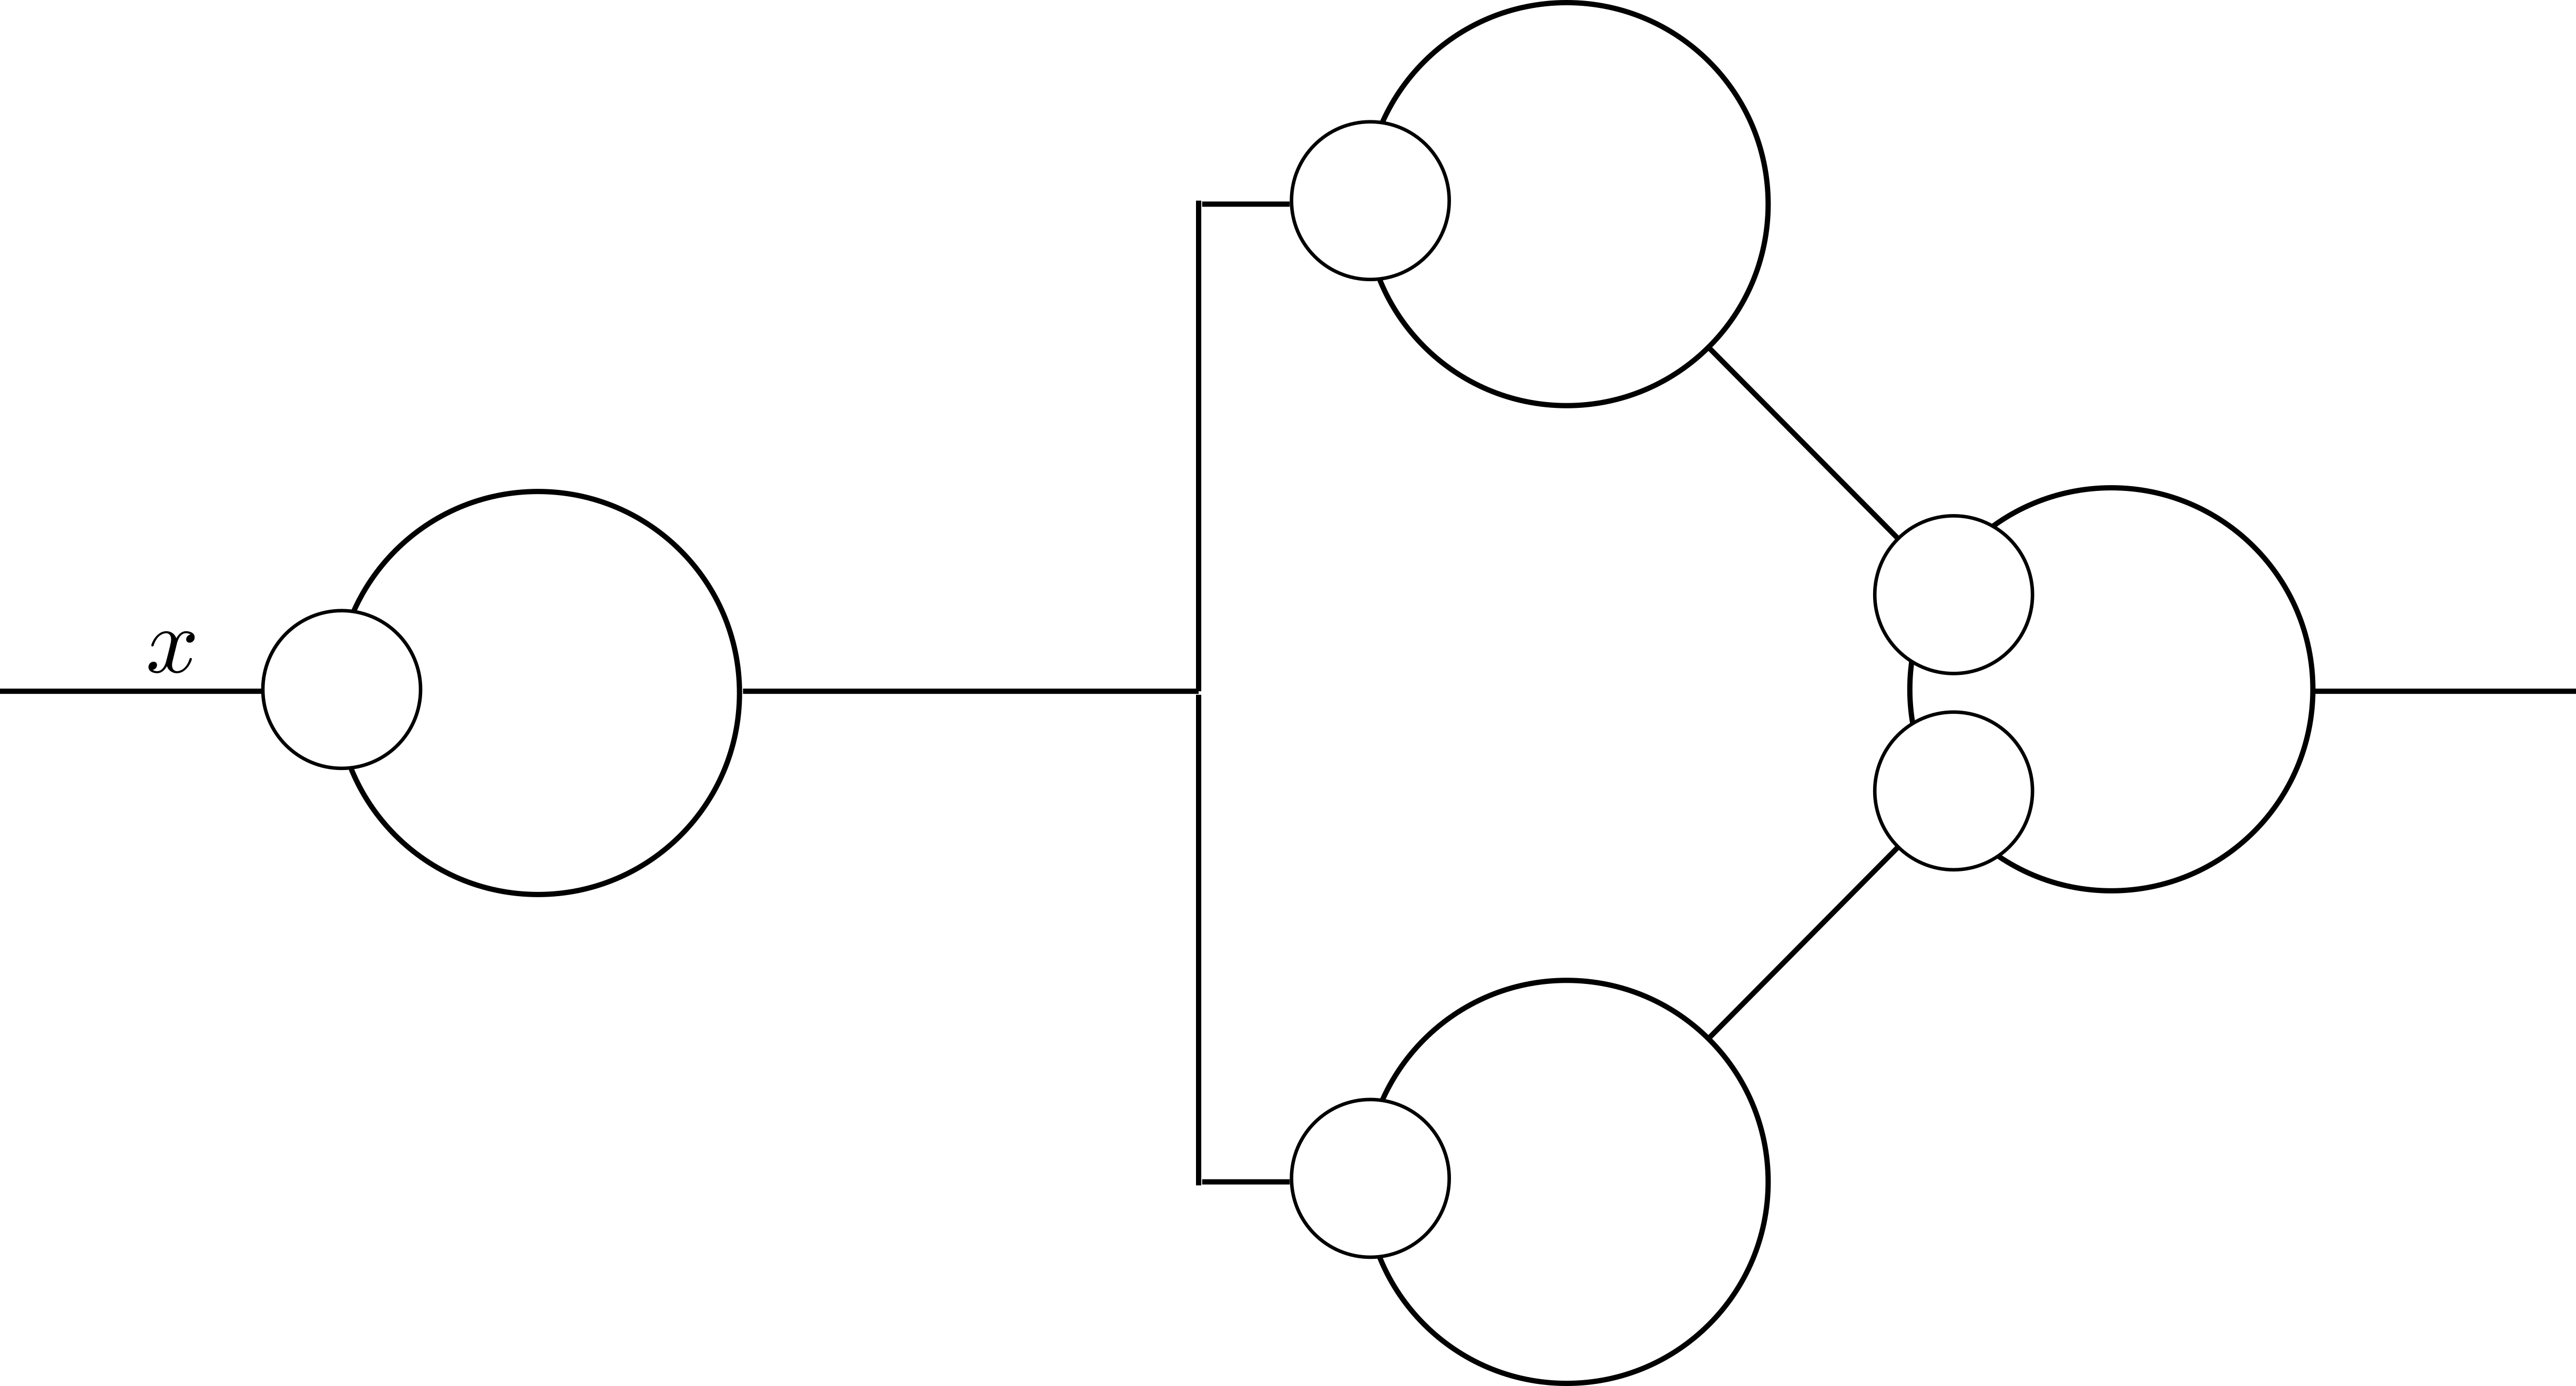
\includegraphics[width=\textwidth]{bp_0.png}}
\only<2>{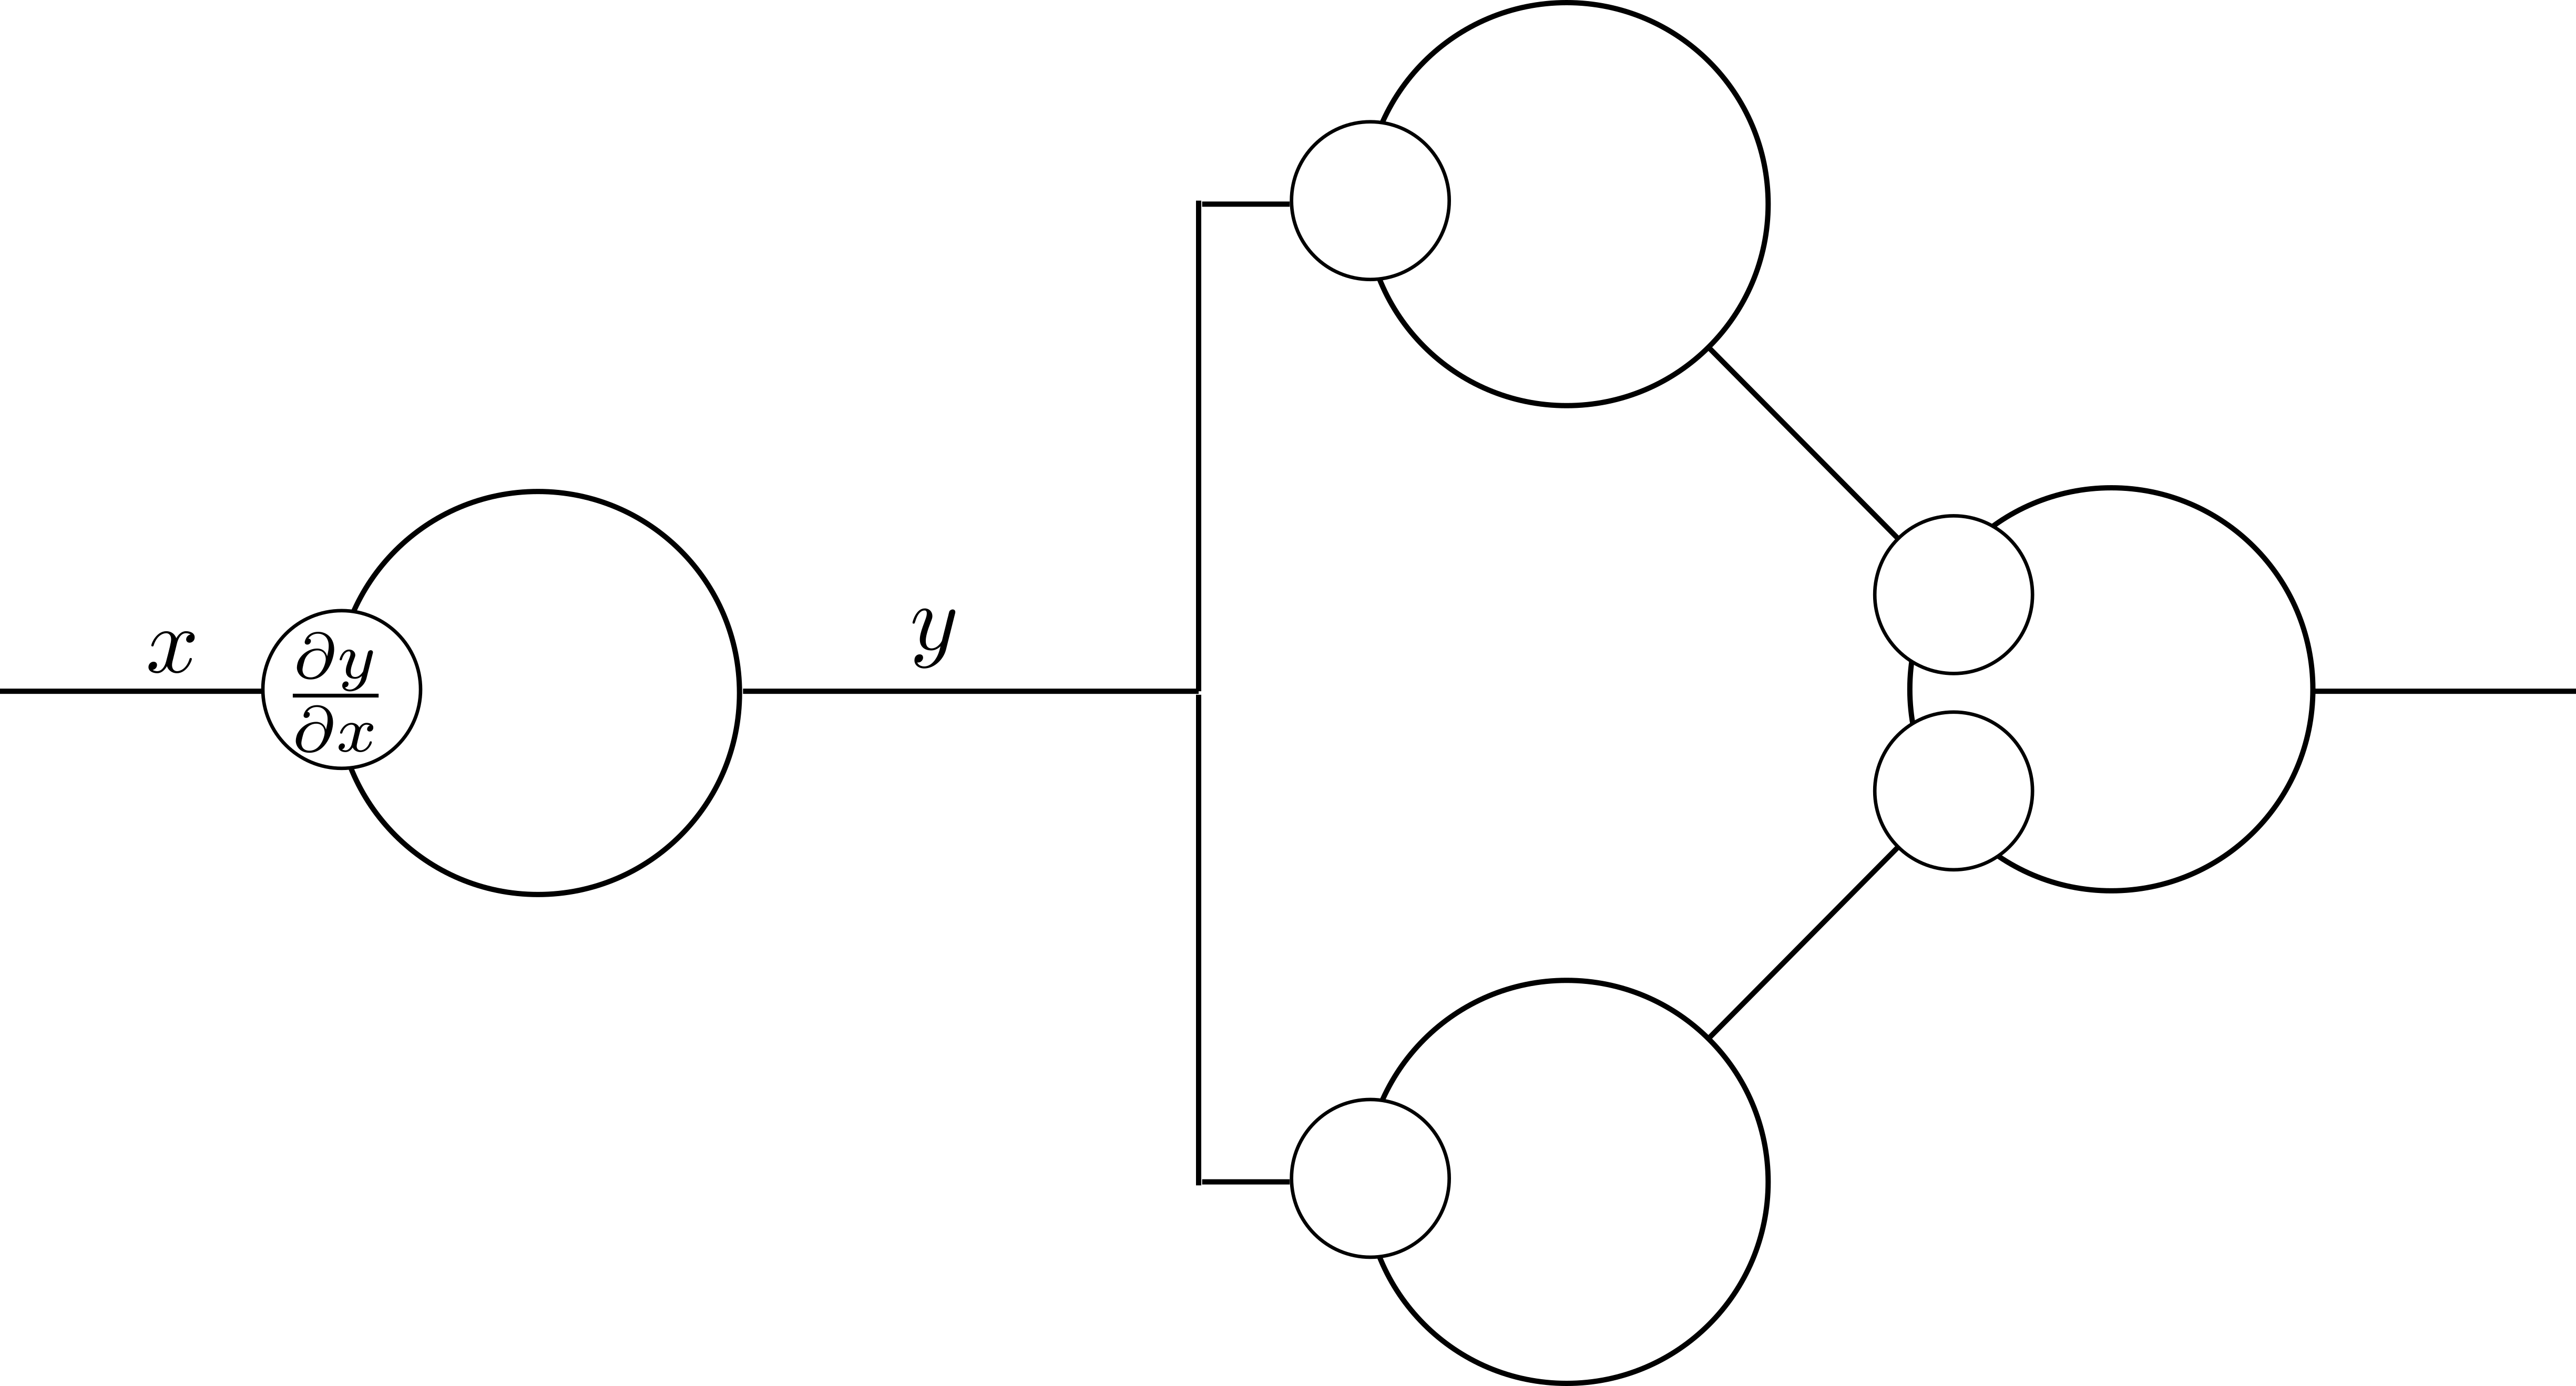
\includegraphics[width=\textwidth]{bp_1.png}}
\only<3>{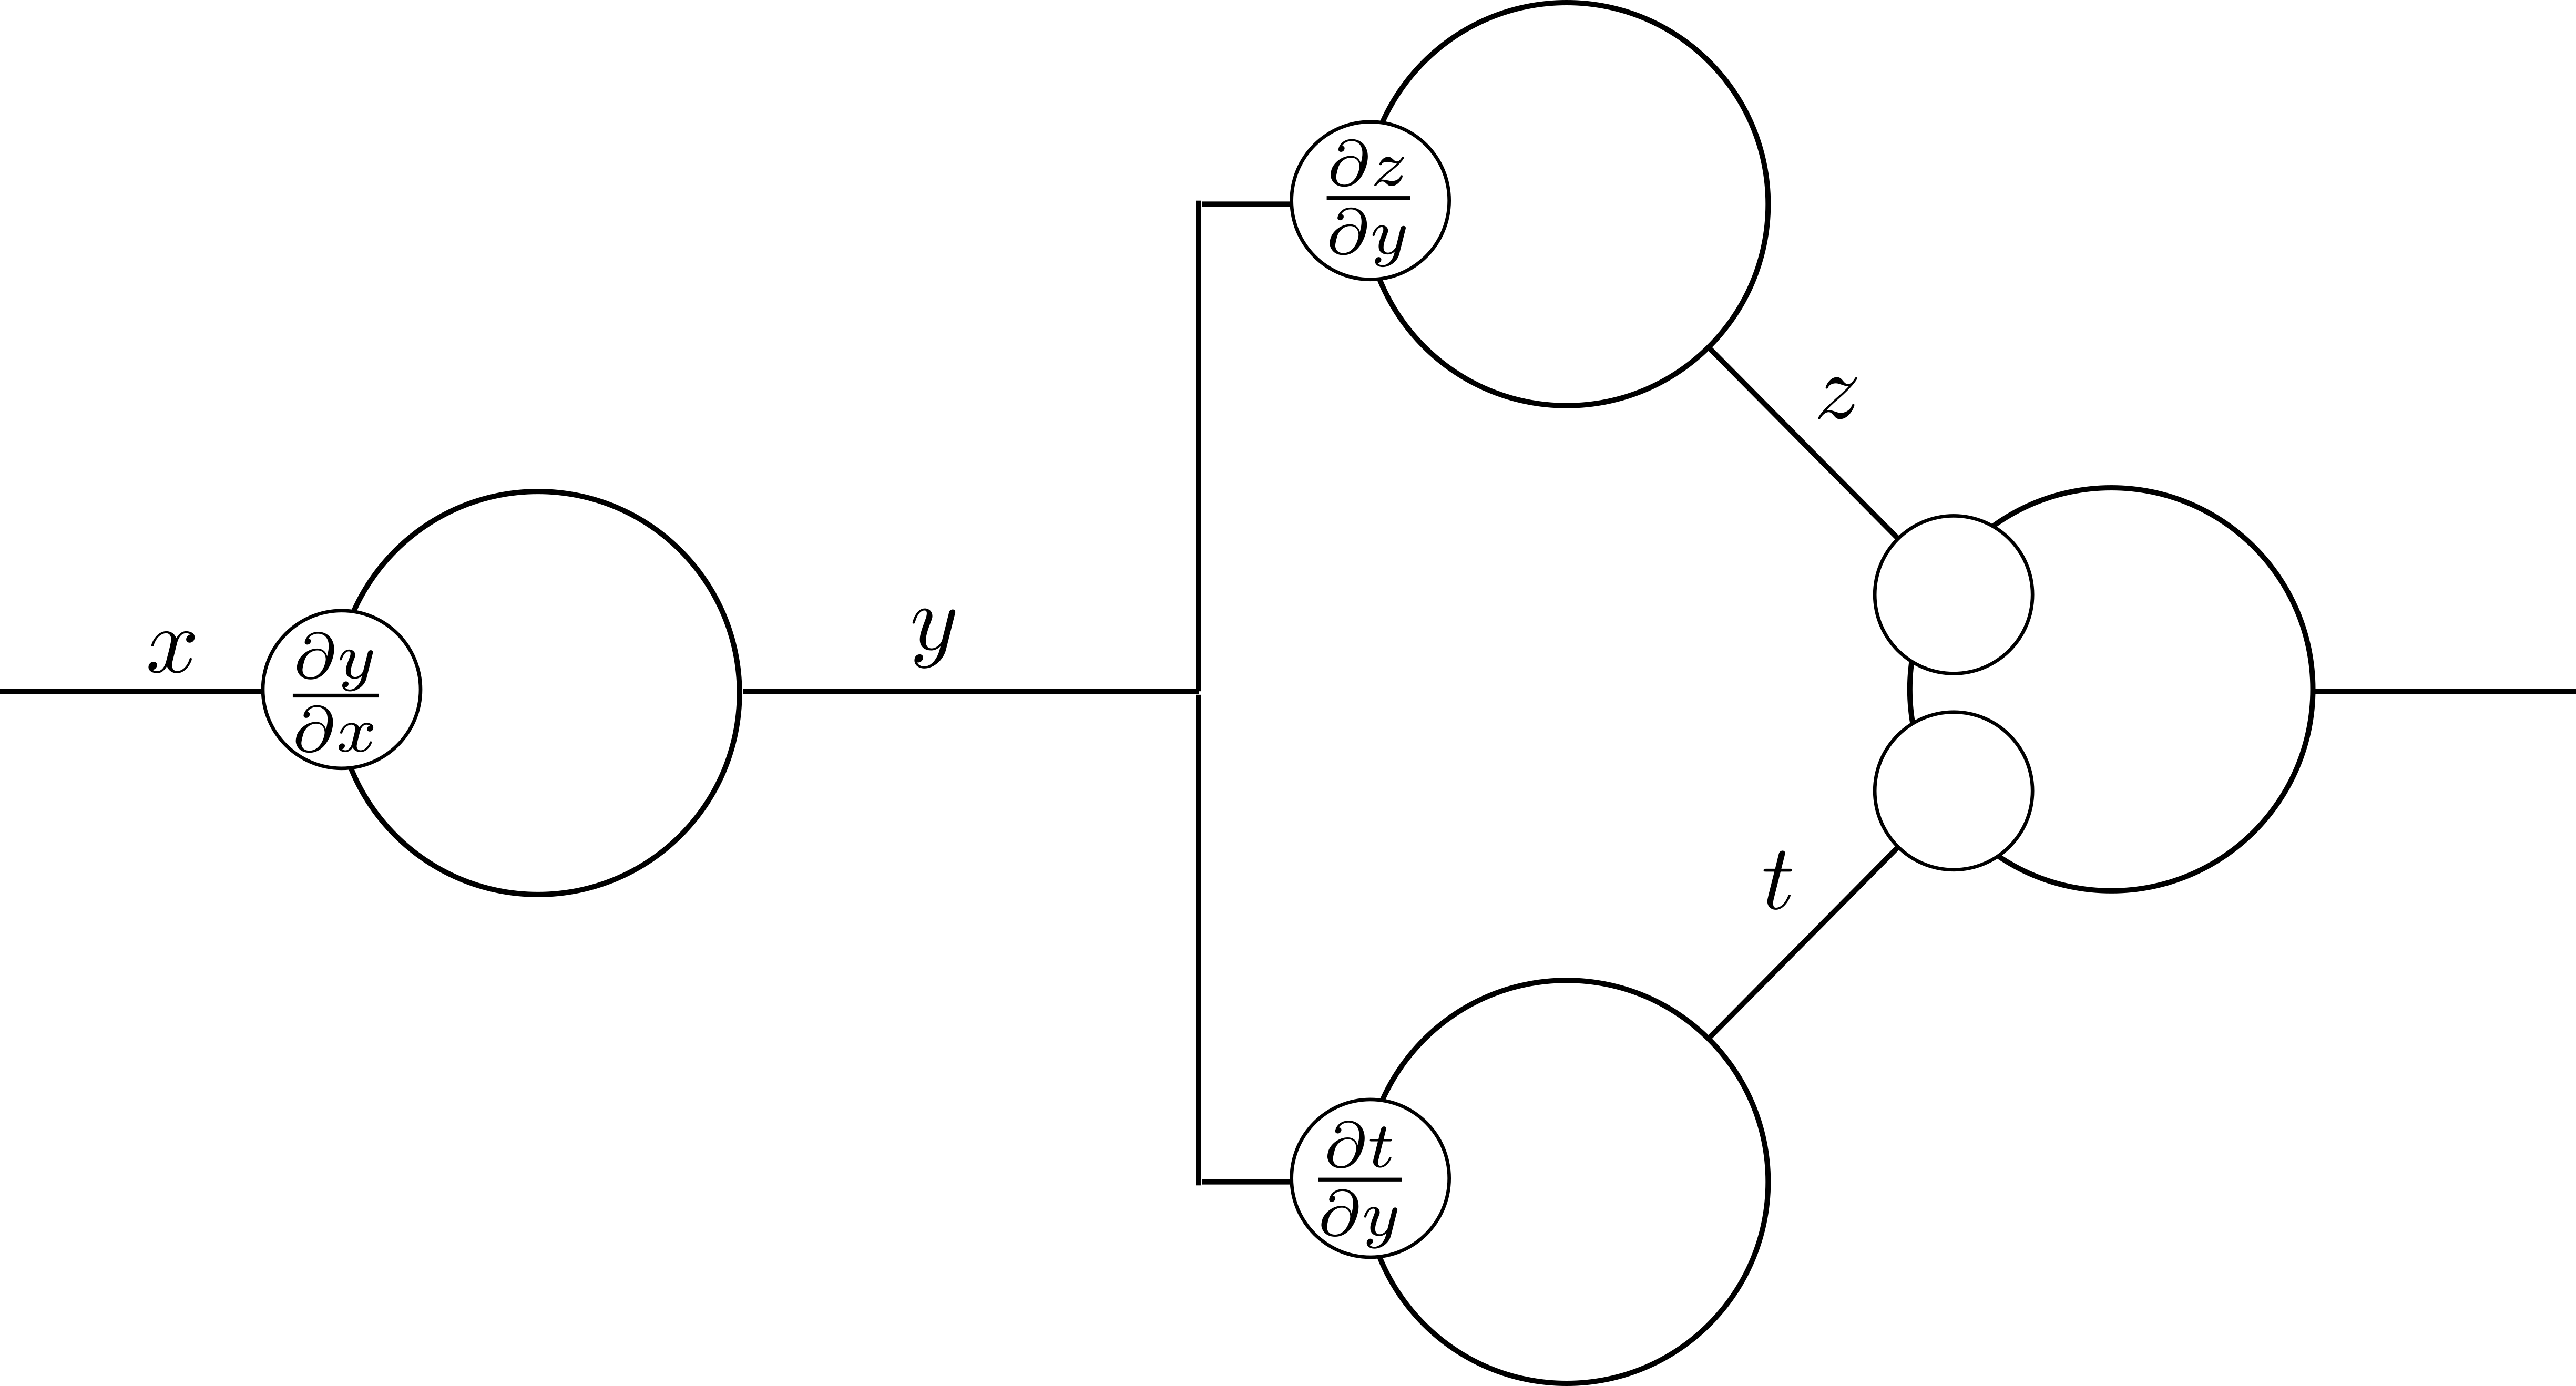
\includegraphics[width=\textwidth]{bp_2.png}}
\only<4>{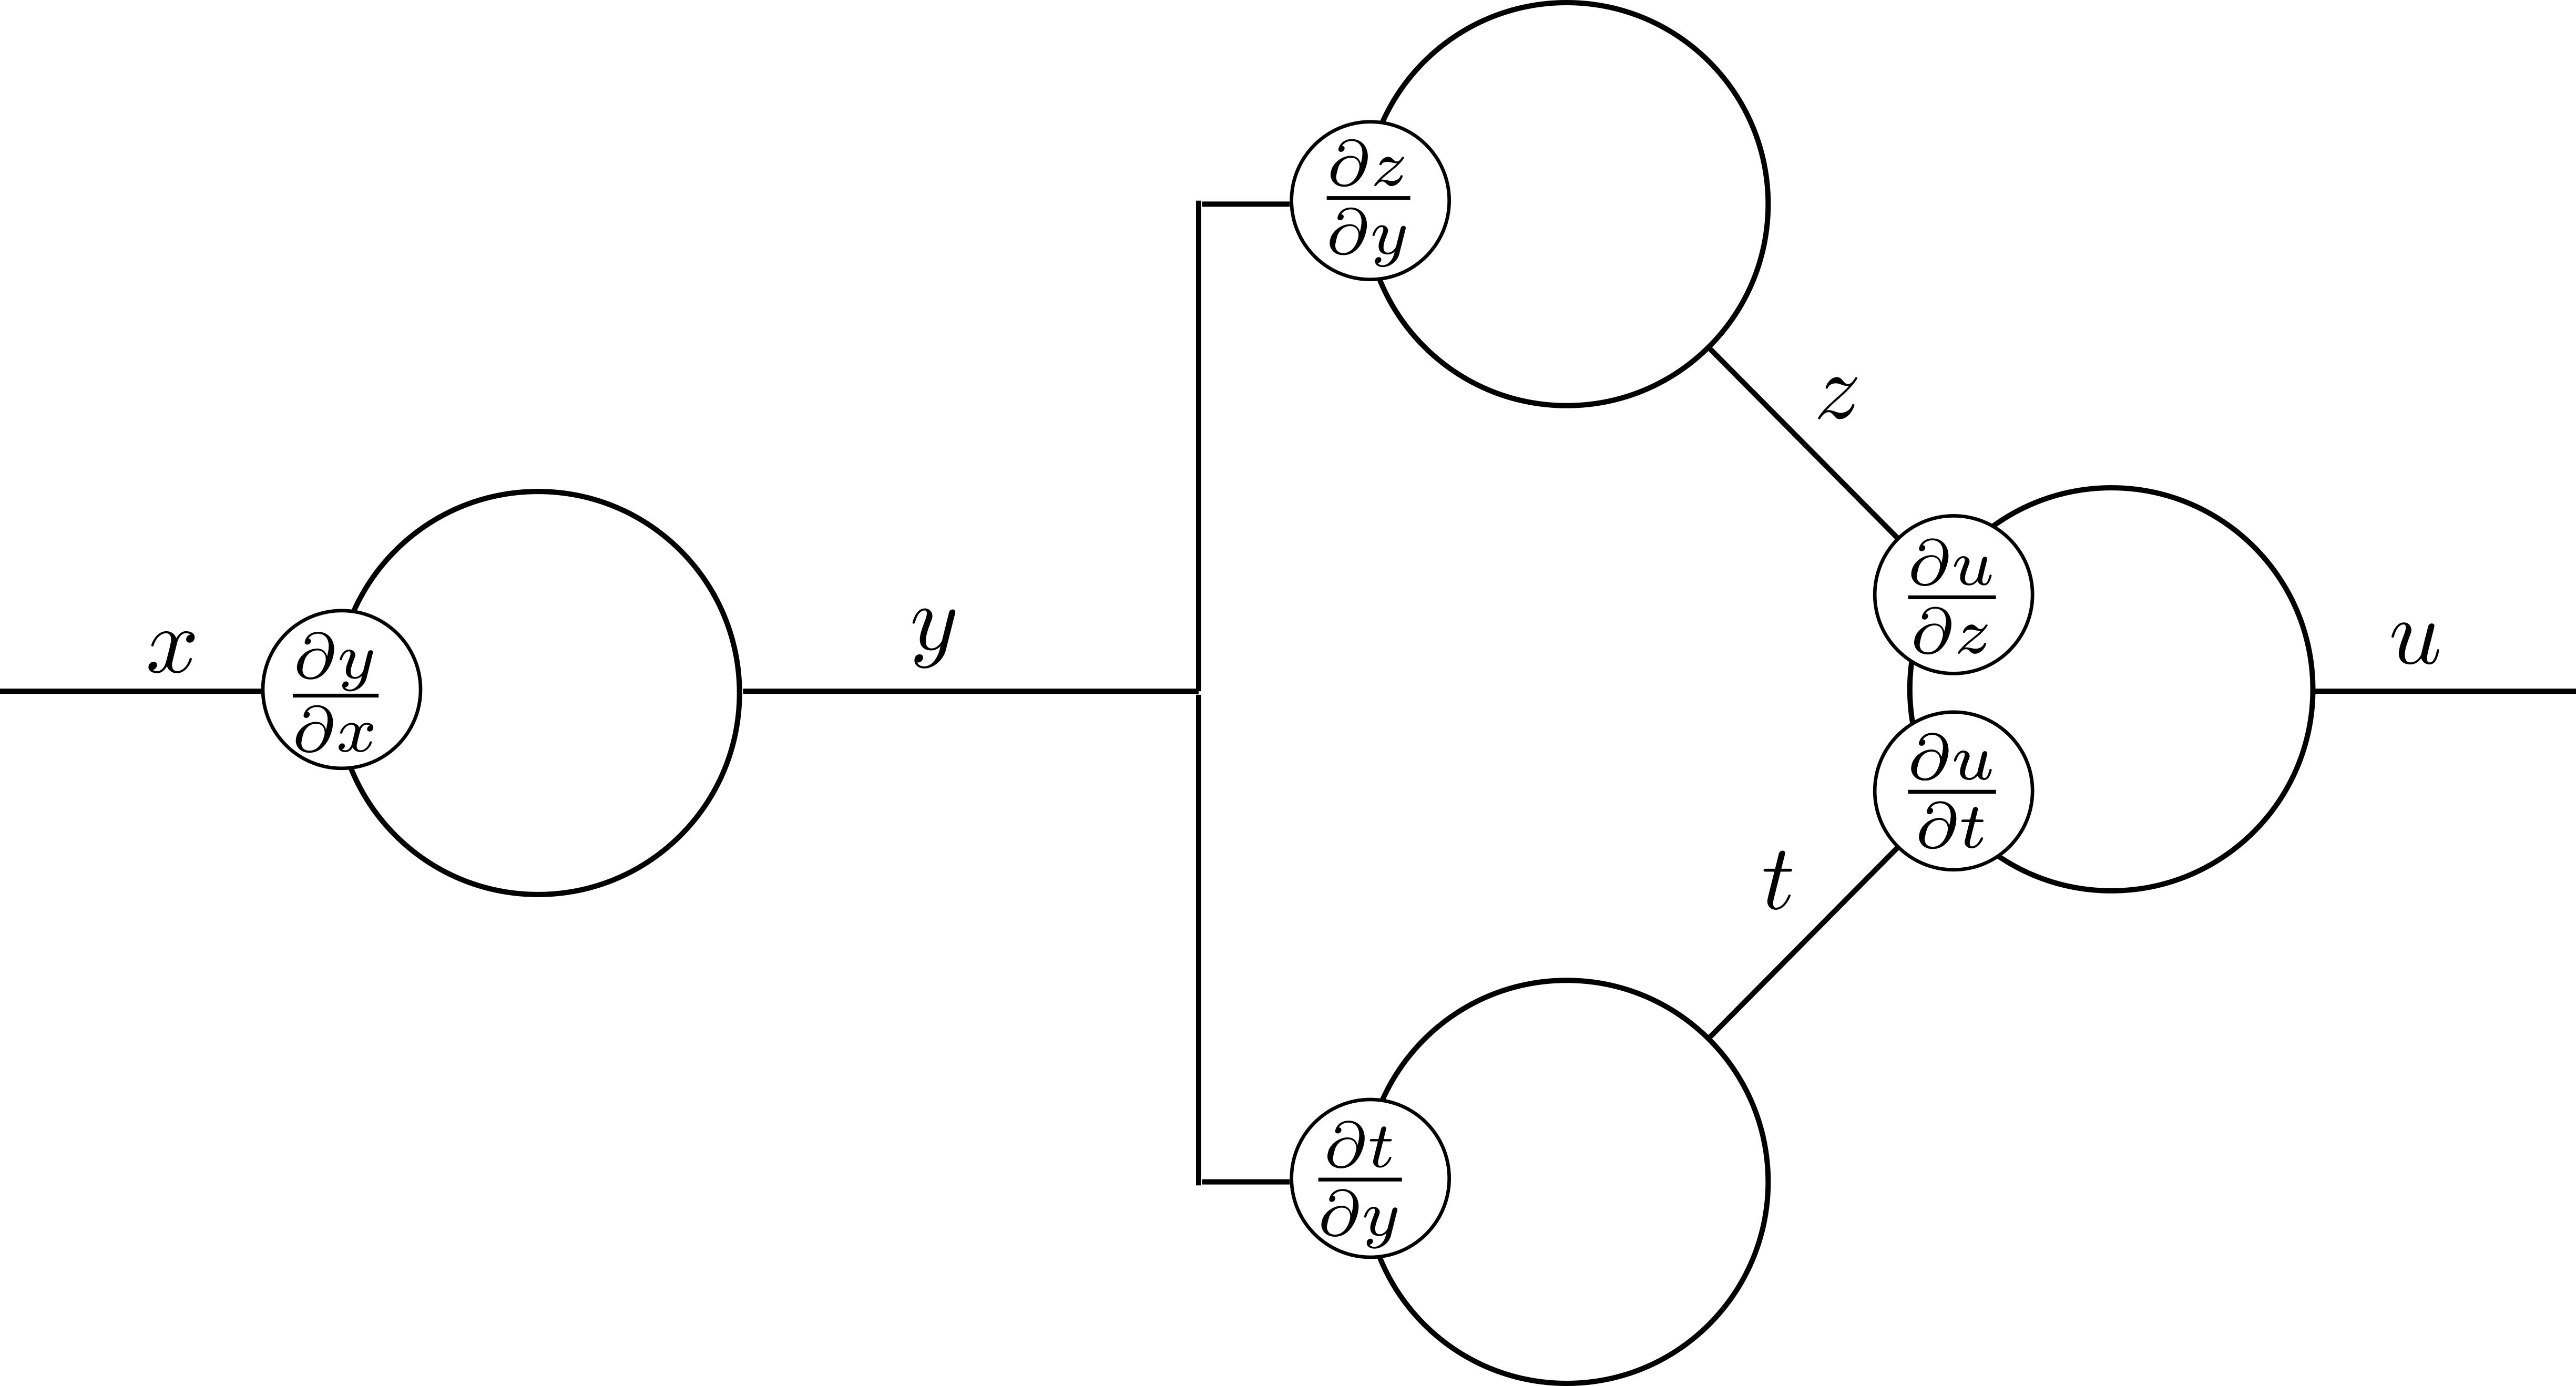
\includegraphics[width=\textwidth]{bp_3.png}}
\only<5>{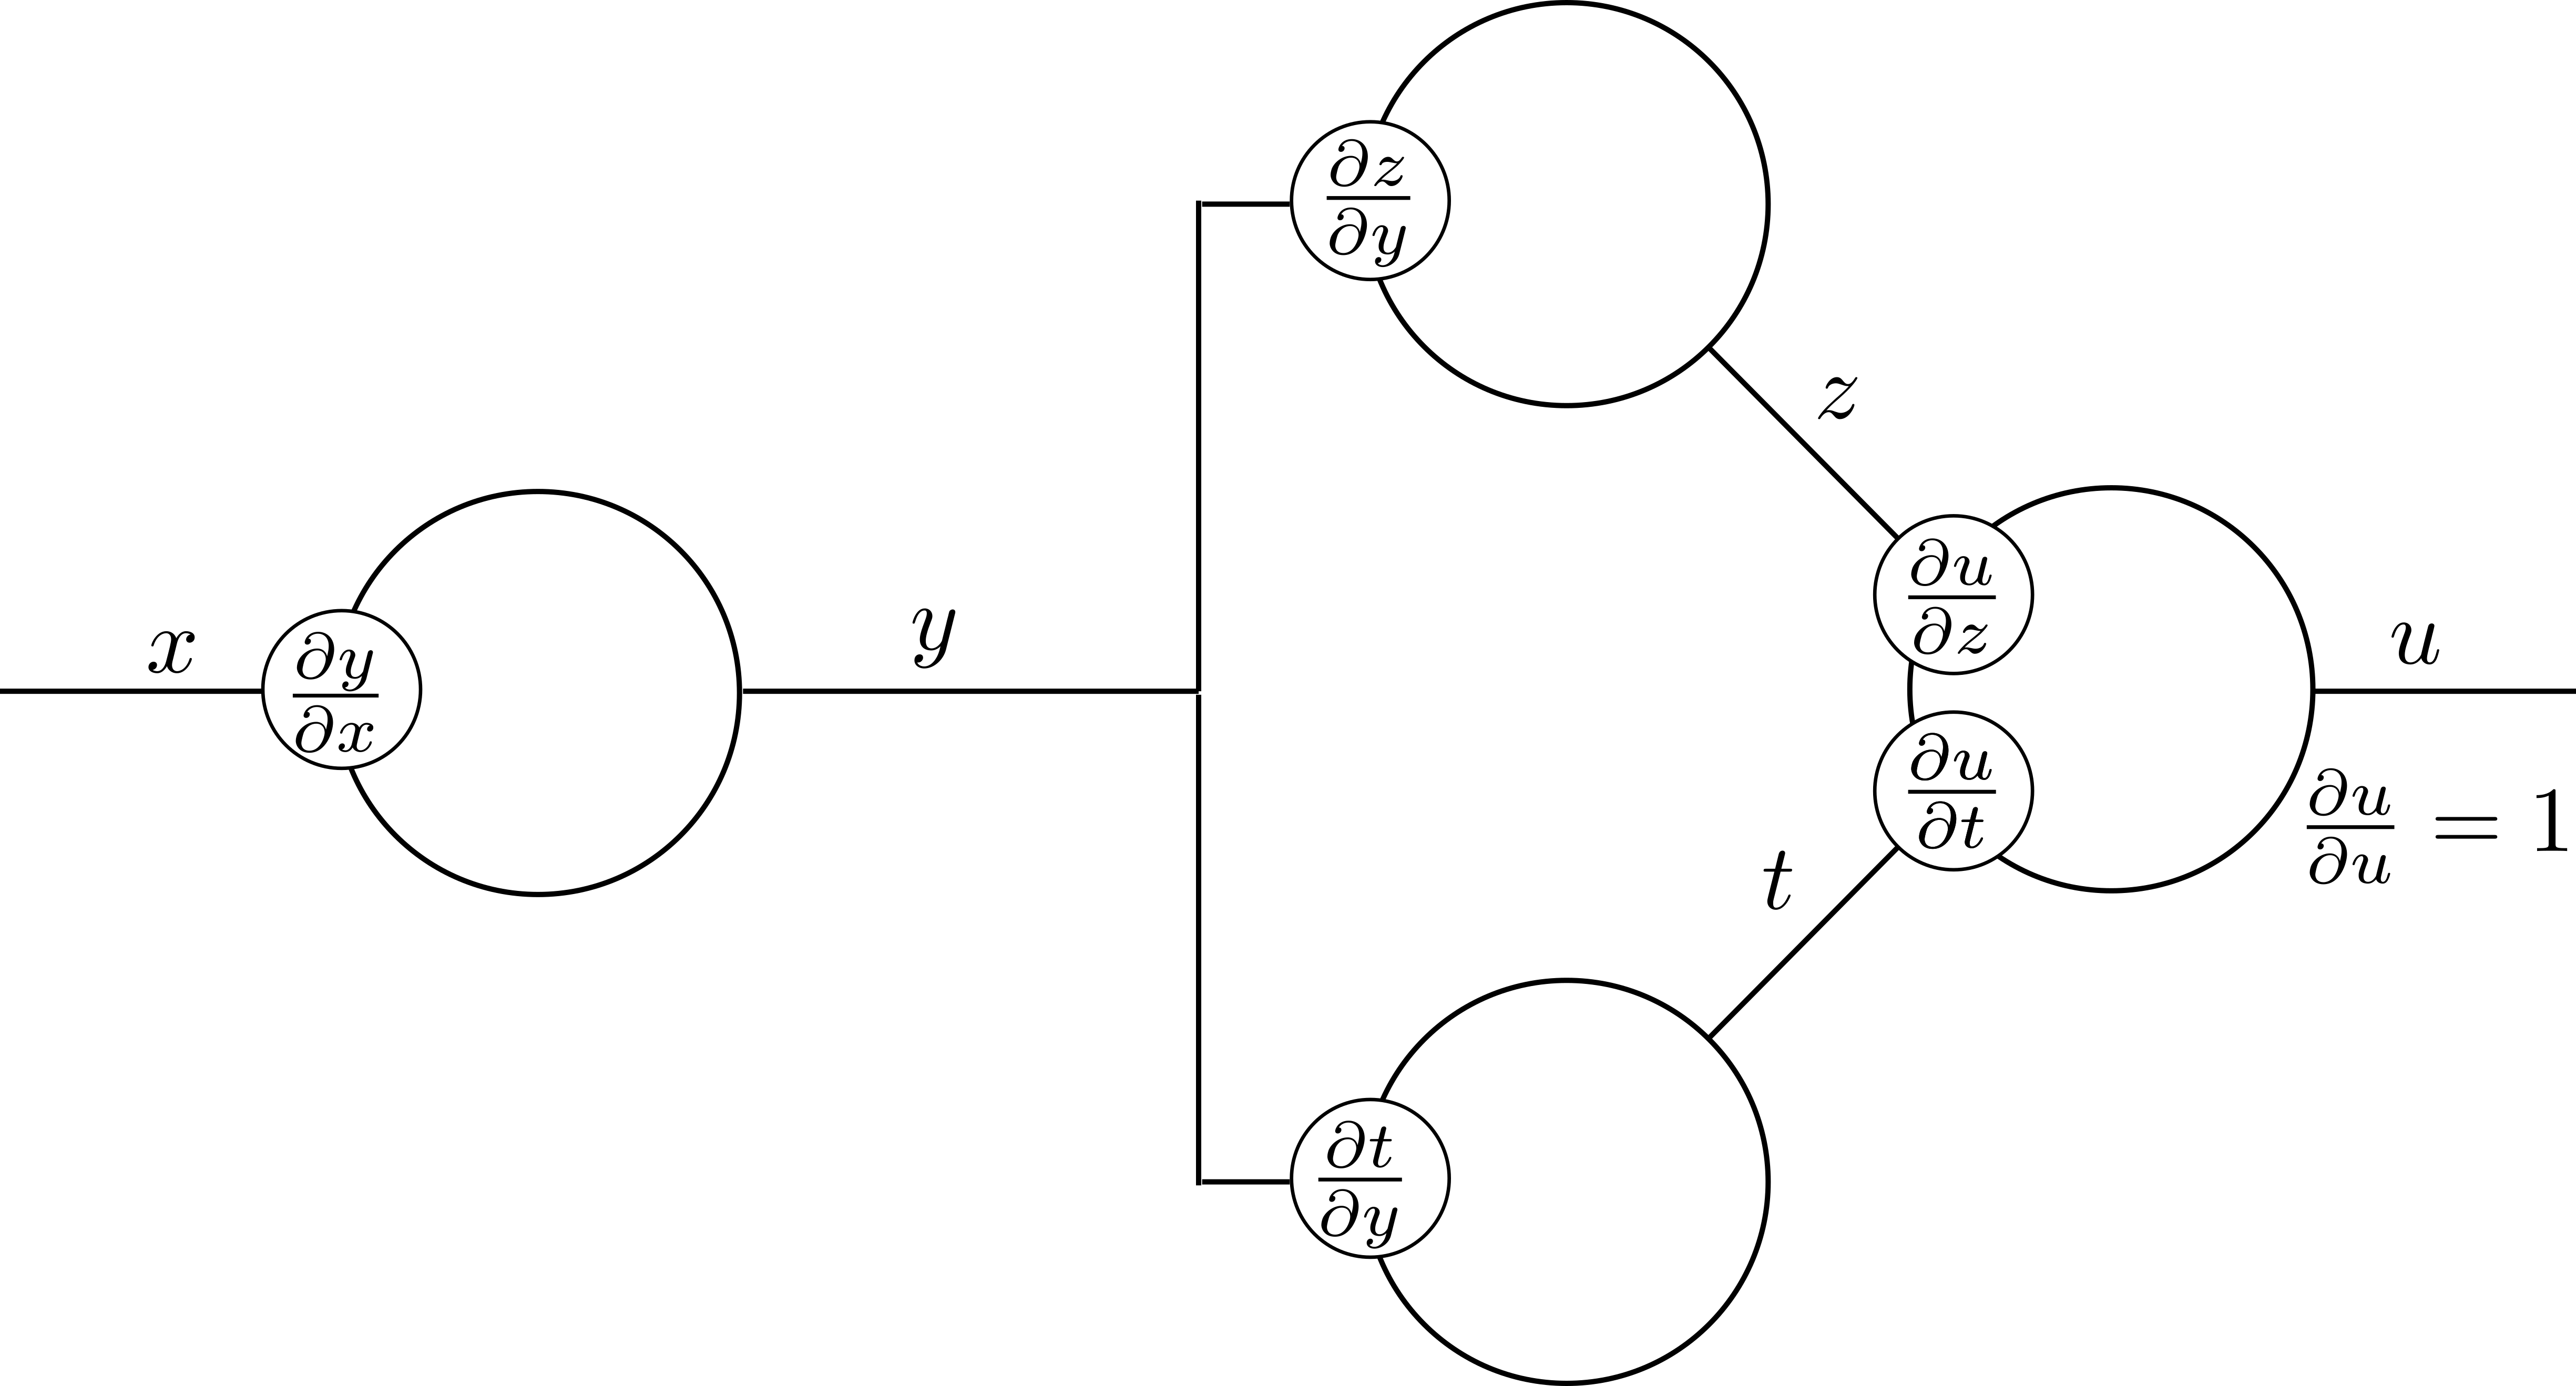
\includegraphics[width=\textwidth]{bp_4.png}}
\only<6>{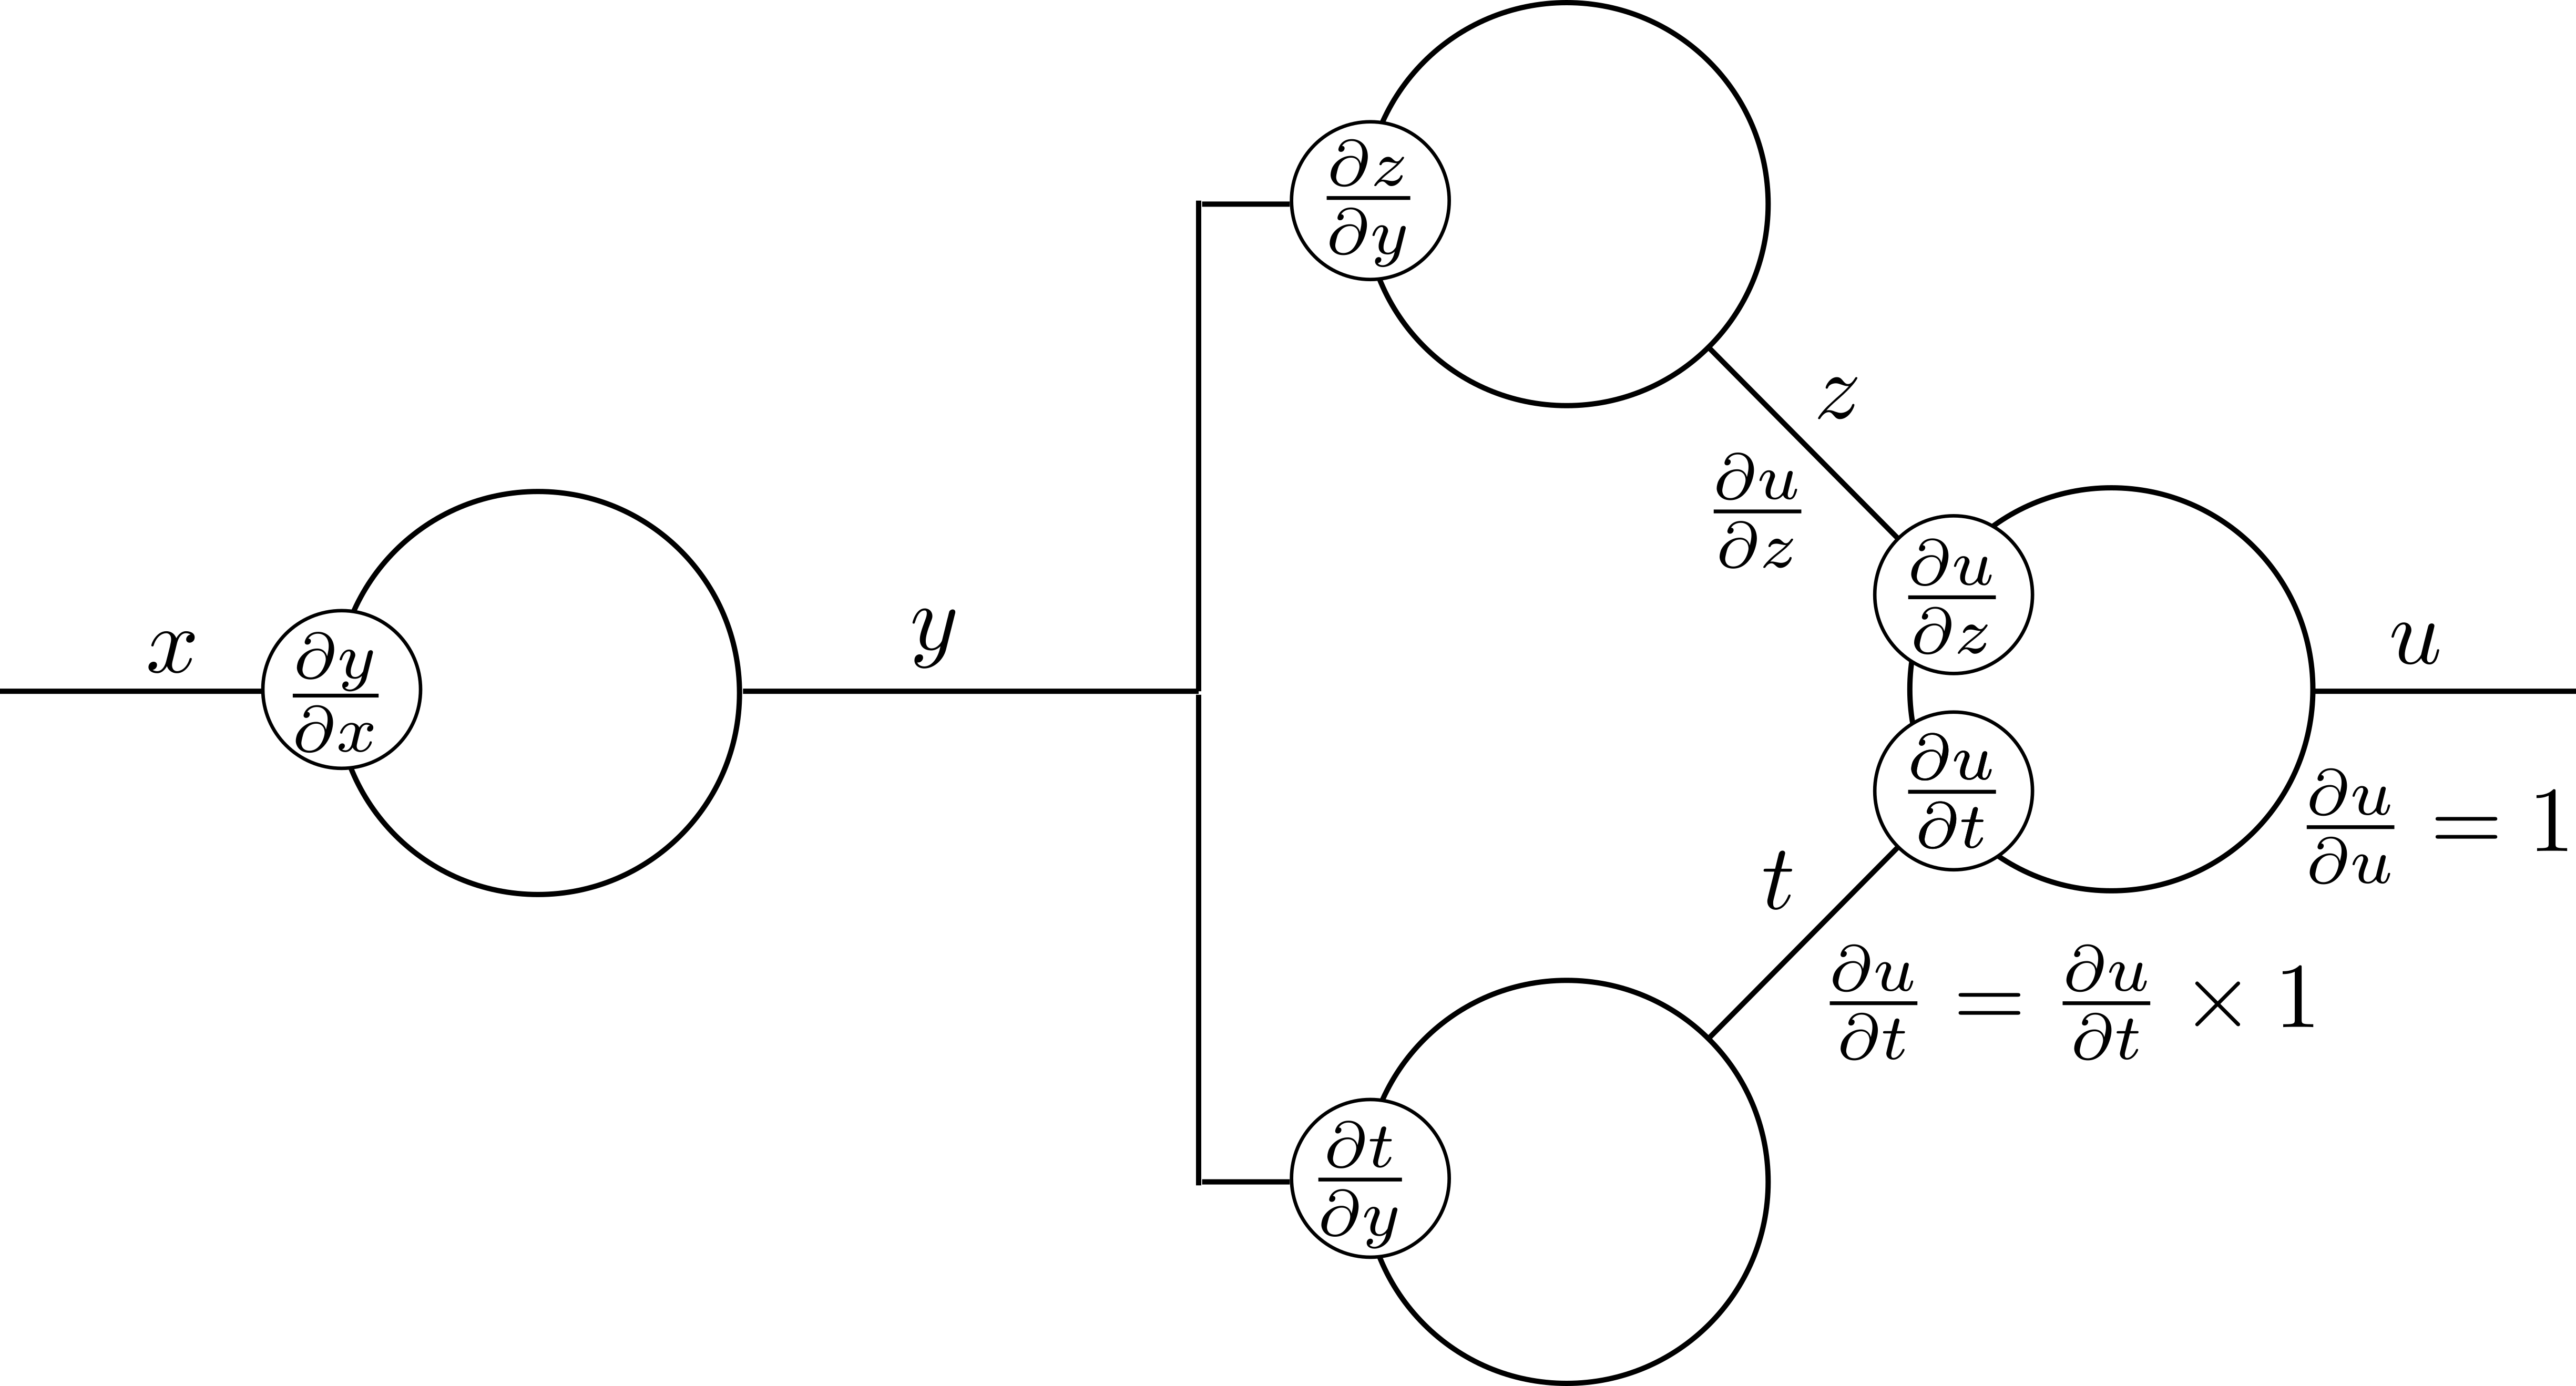
\includegraphics[width=\textwidth]{bp_5.png}}
\only<7>{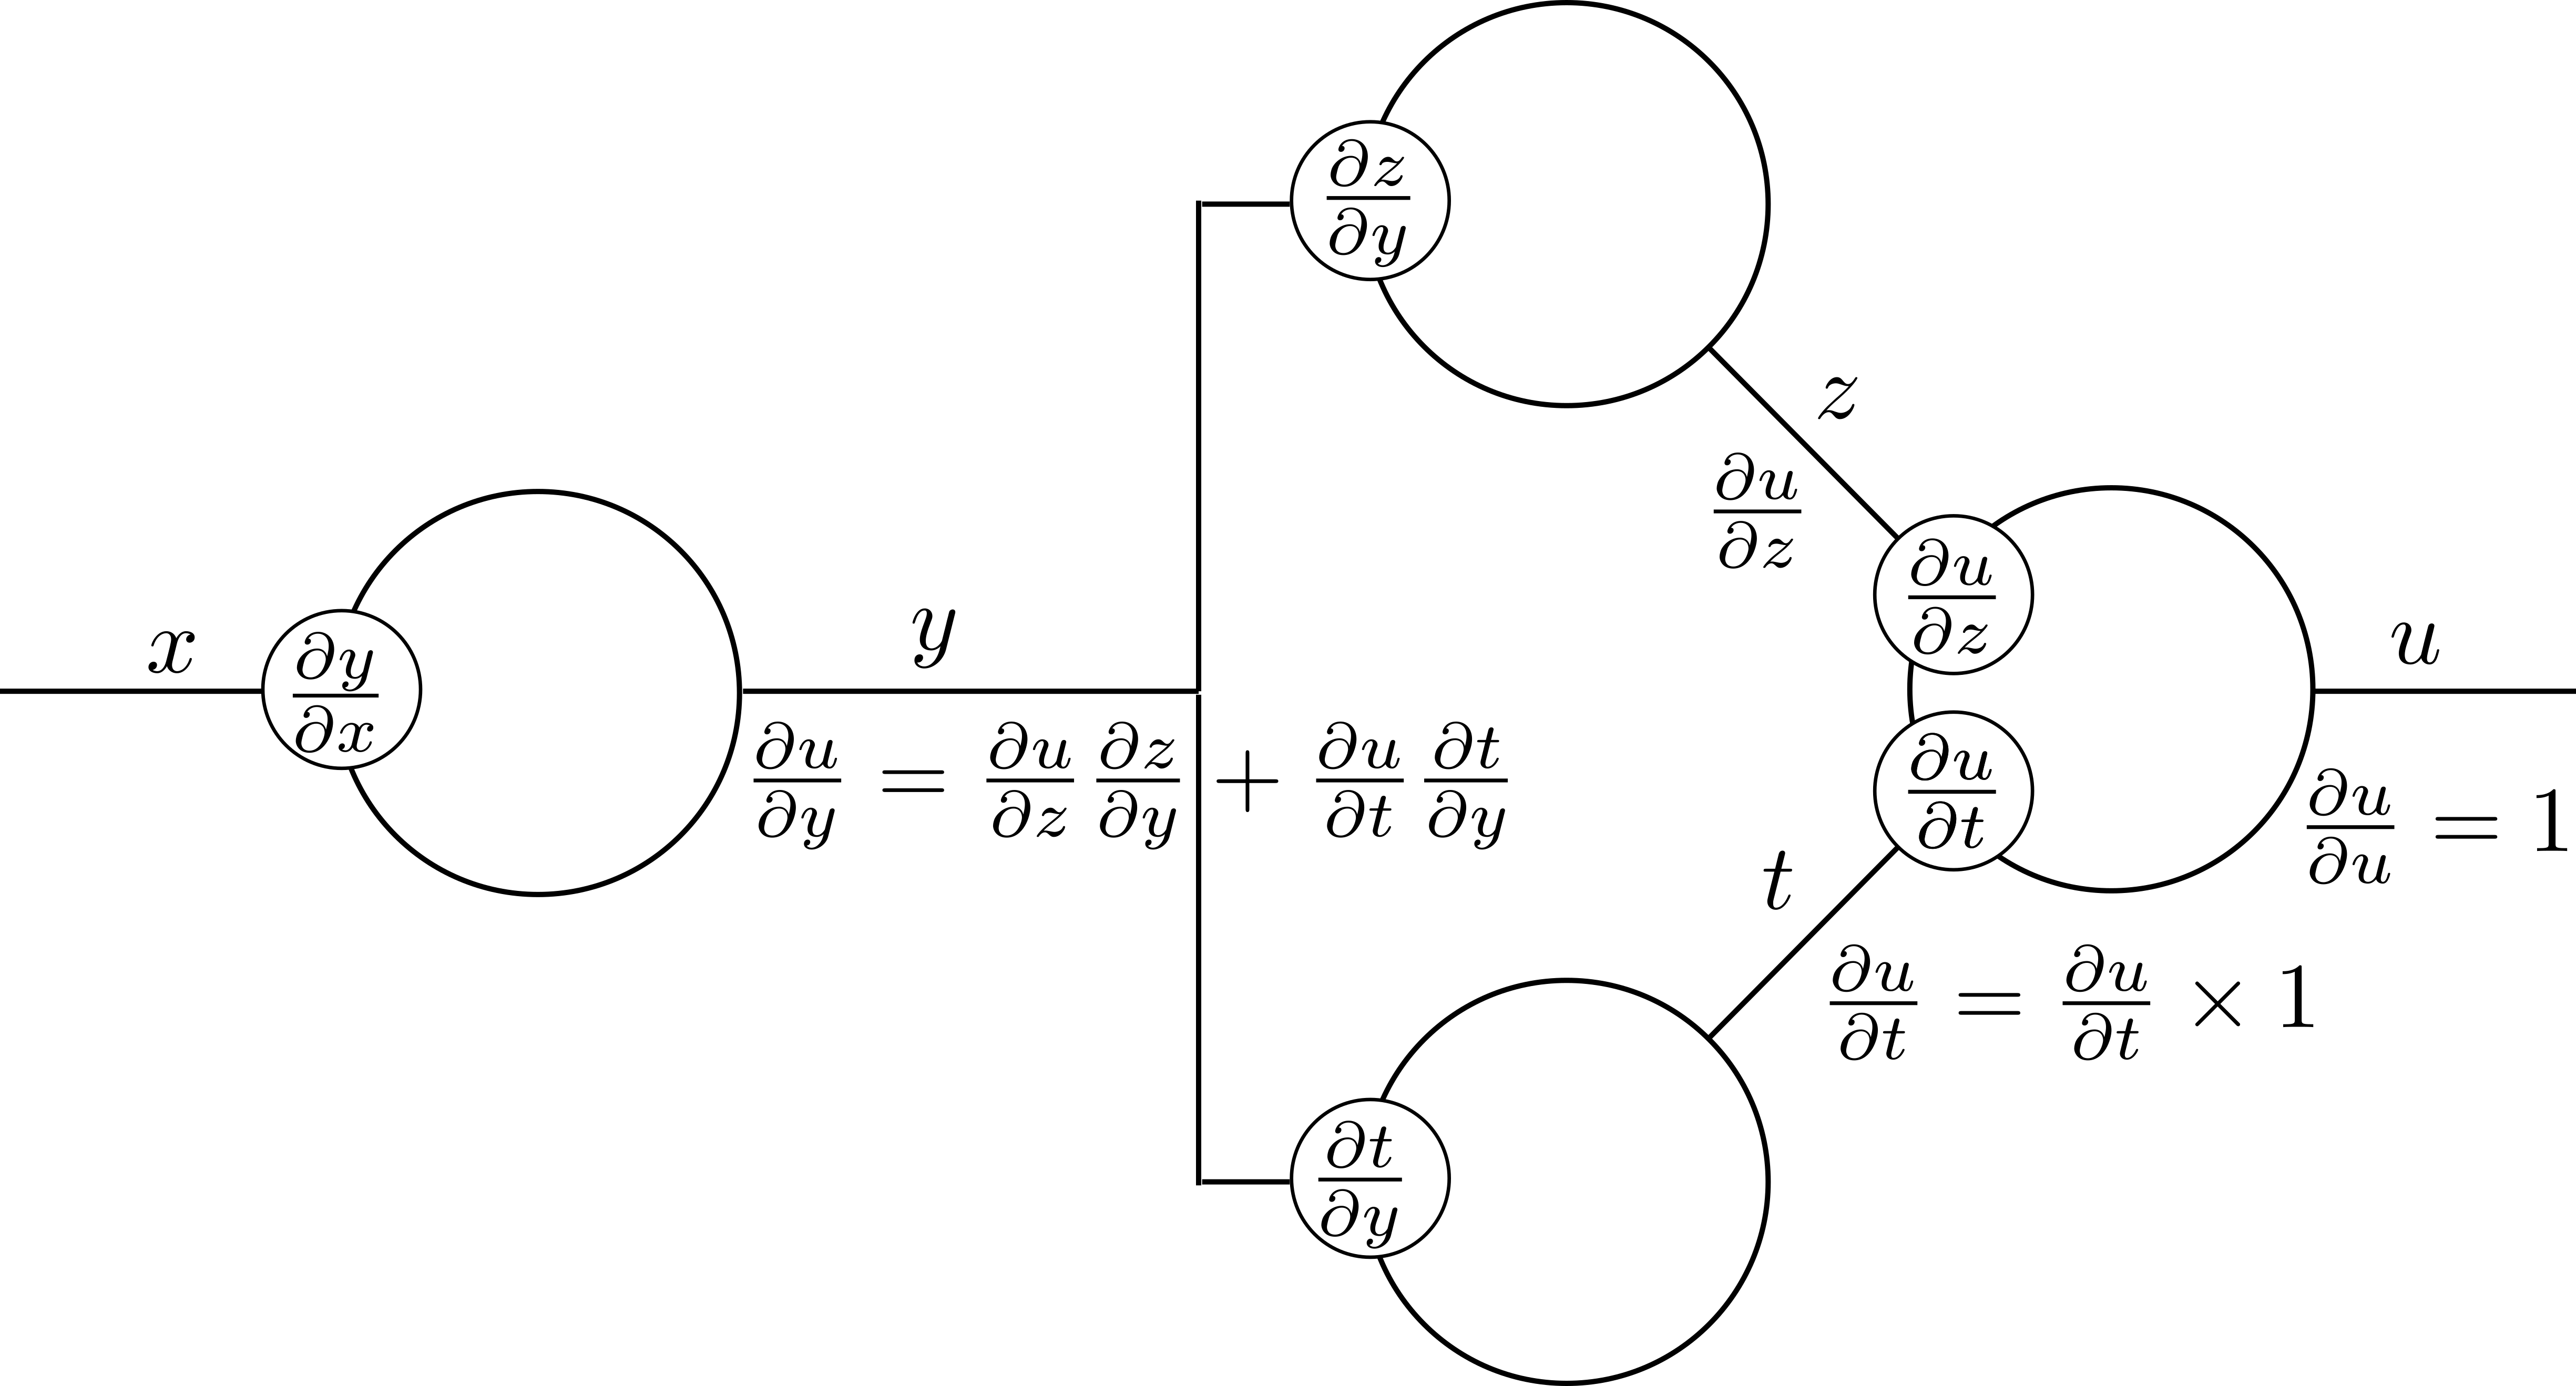
\includegraphics[width=\textwidth]{bp_6.png}}
\only<8>{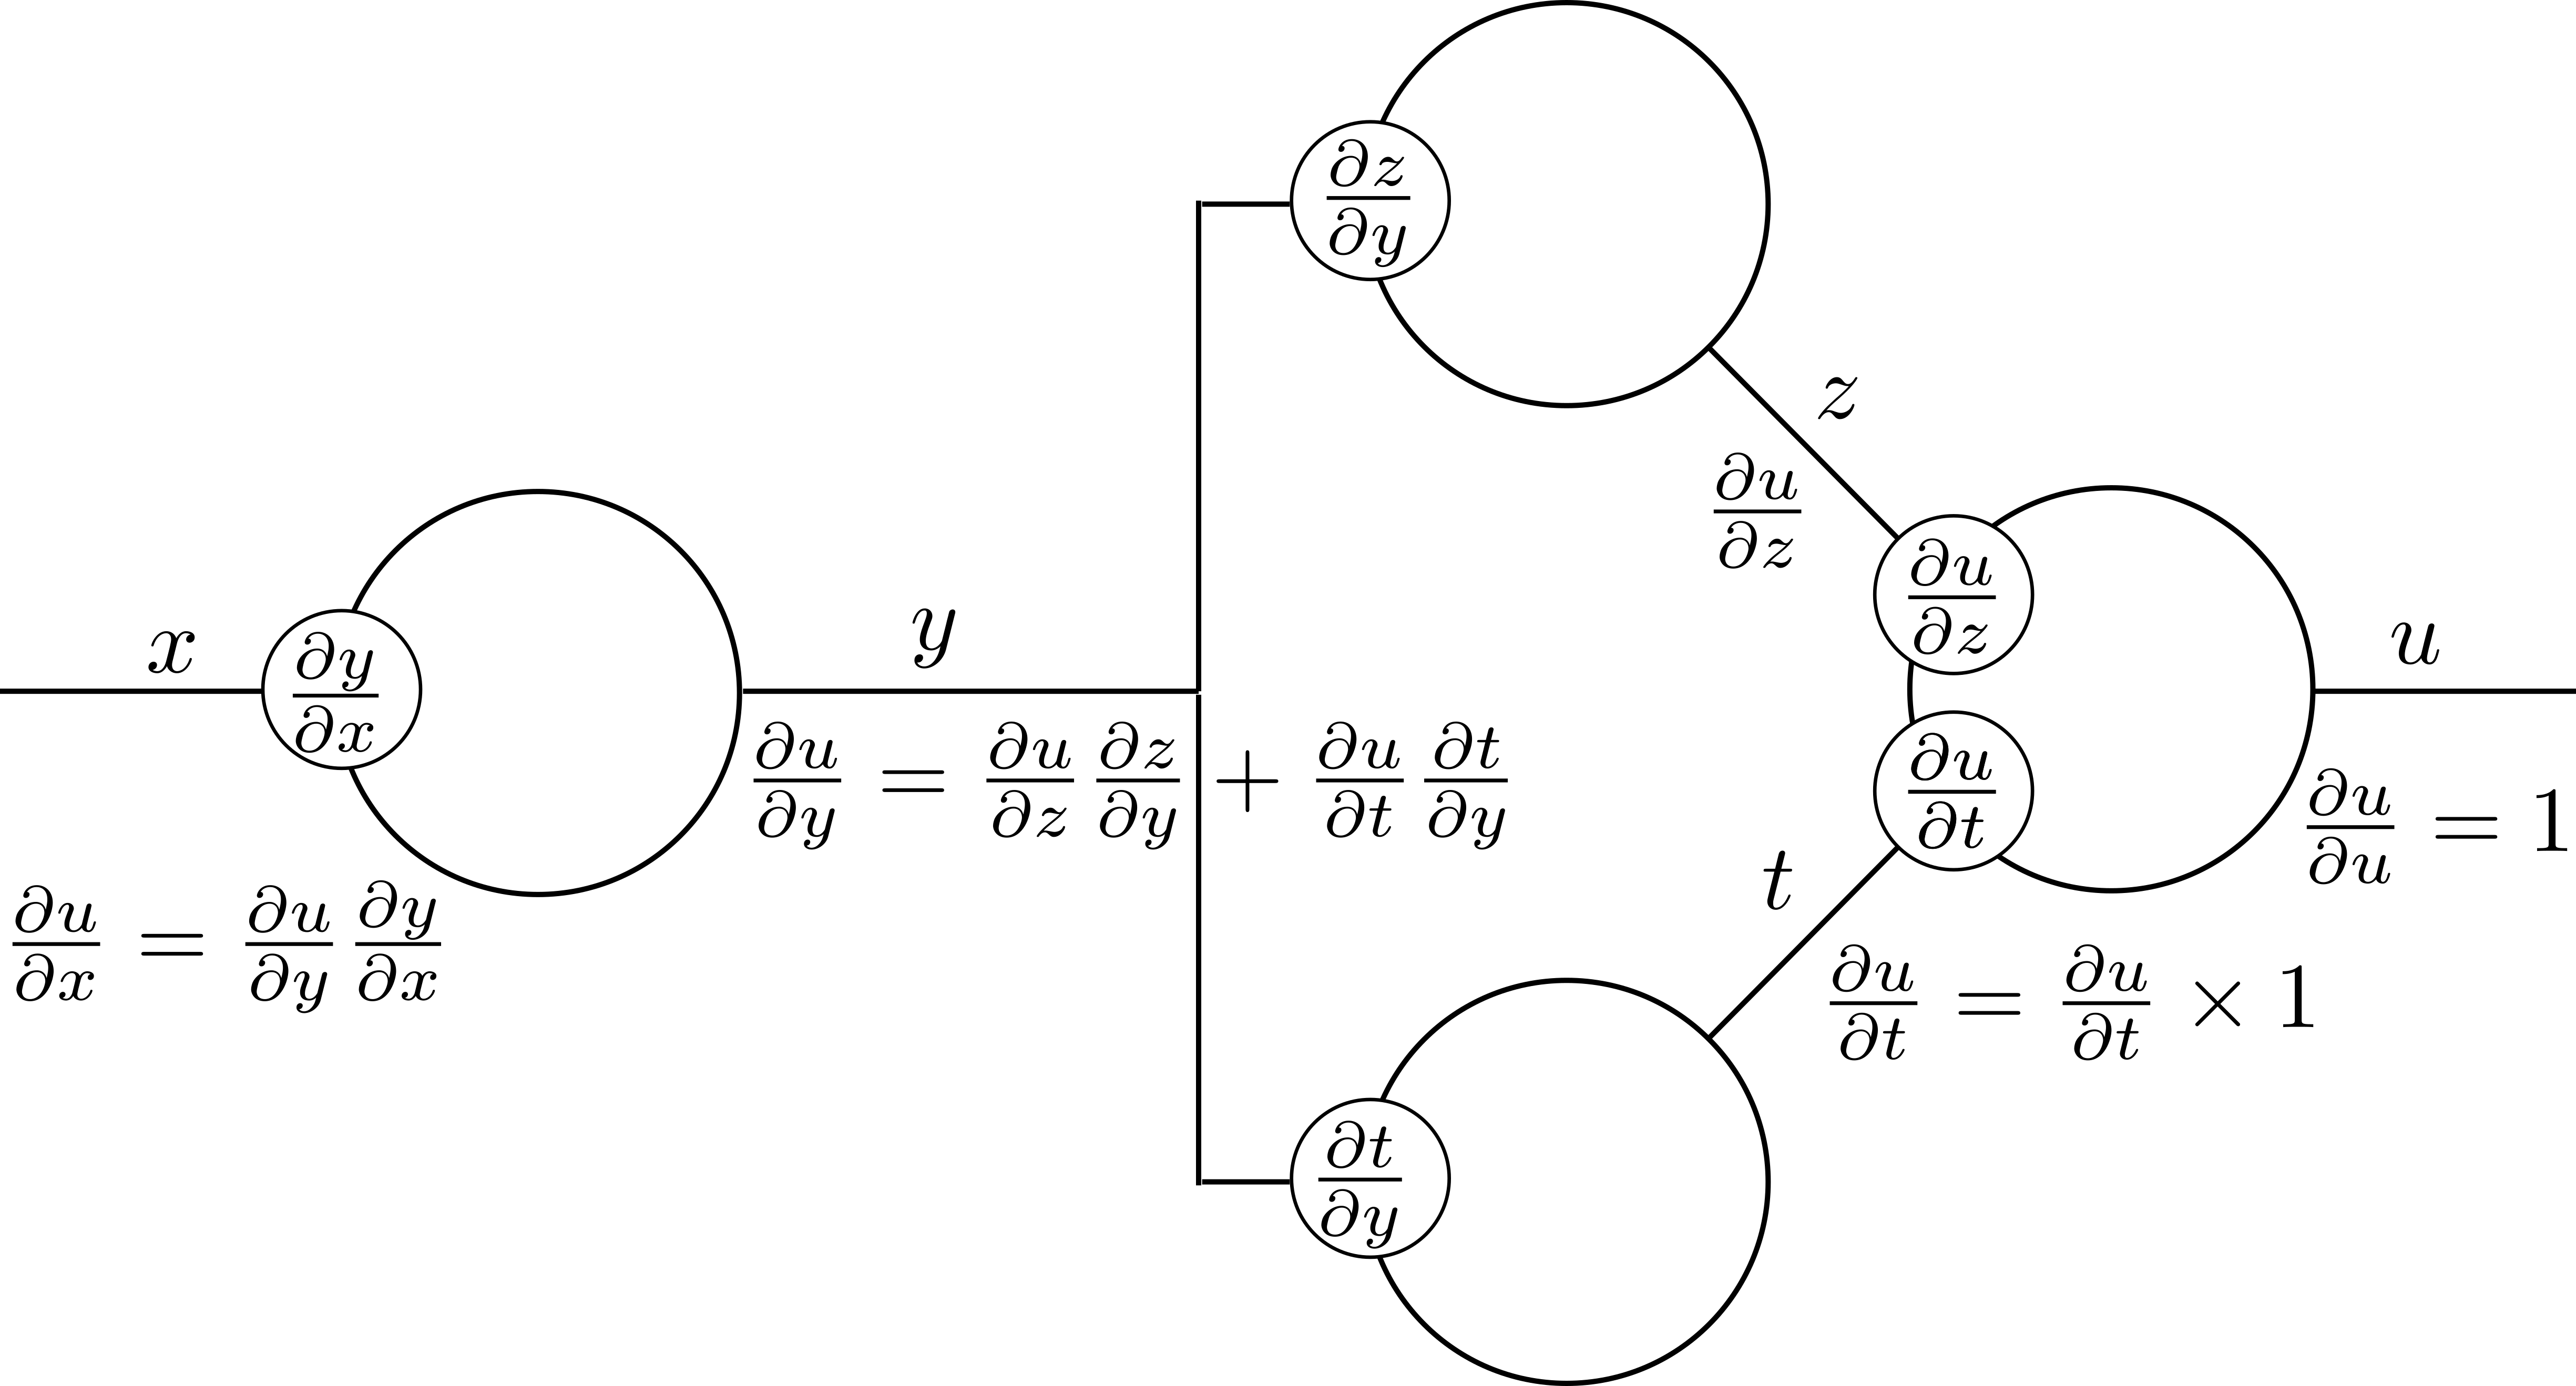
\includegraphics[width=\textwidth]{bp_7.png}}

\end{frame}



%%%%%%%%%%%%%%%%%%%%%%%%%%%%%%%%%%%%
%% \begin{frame}{Simple backpropagation example}

%%   \animategraphics[width=4cm, step]{1}{bp_}{0}{7}

%% \end{frame}


%%%%%%%%%%%%%%%%%%%%%%%%%%%%%%%%%%%%%%%%%%%%%%%%%
\begin{frame}{Backpropagation through a fully connected layer}
\begin{figure}
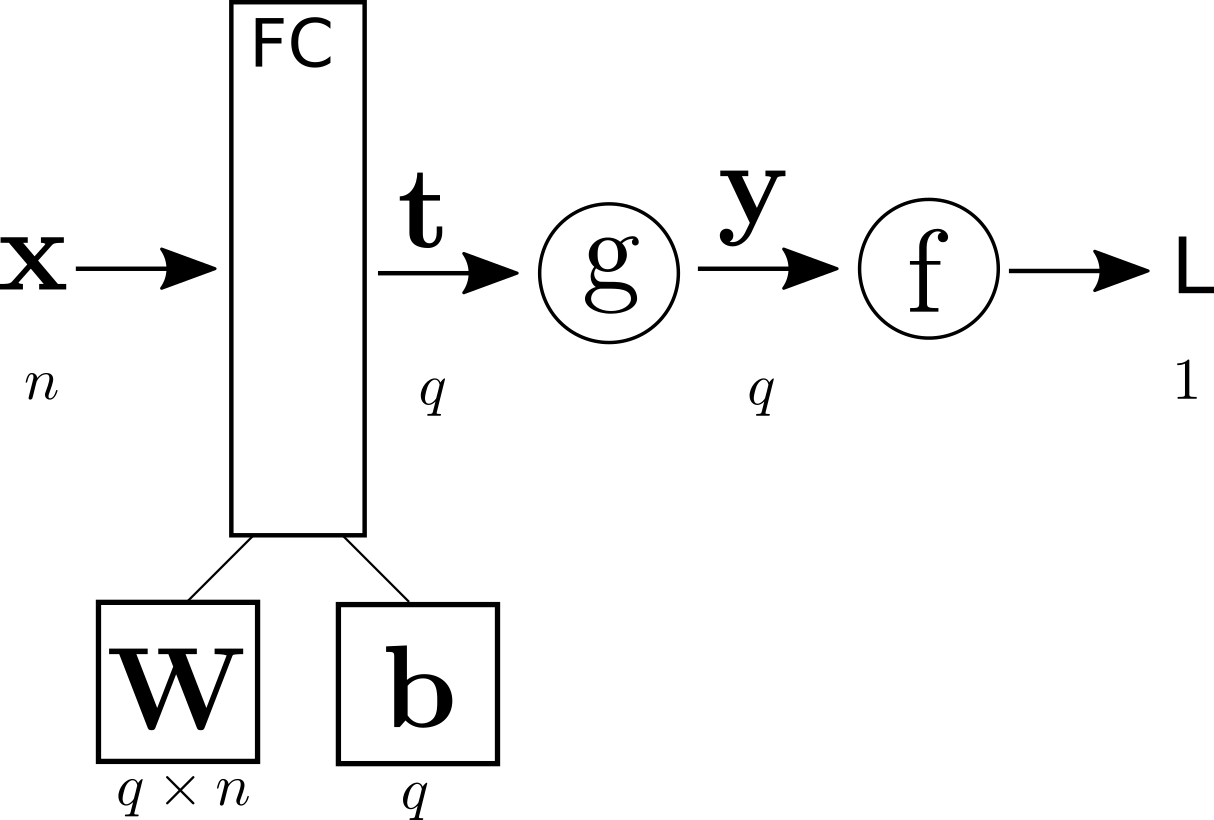
\includegraphics[width=0.5\textwidth]{bp_fc.png}
\end{figure}

Setup:
\begin{eqnarray*}
p, q \in \N^*\\
\x \in \R^p \\
\W \in \R^q \times \R^p \\
\bias, \mathbf{t}, \y \in \R^q \\
\loss \in \R
\end{eqnarray*}

\end{frame}

%%%%%%%%%%%%%
\begin{frame}{Backpropagation through a fully connected layer}
\begin{figure}
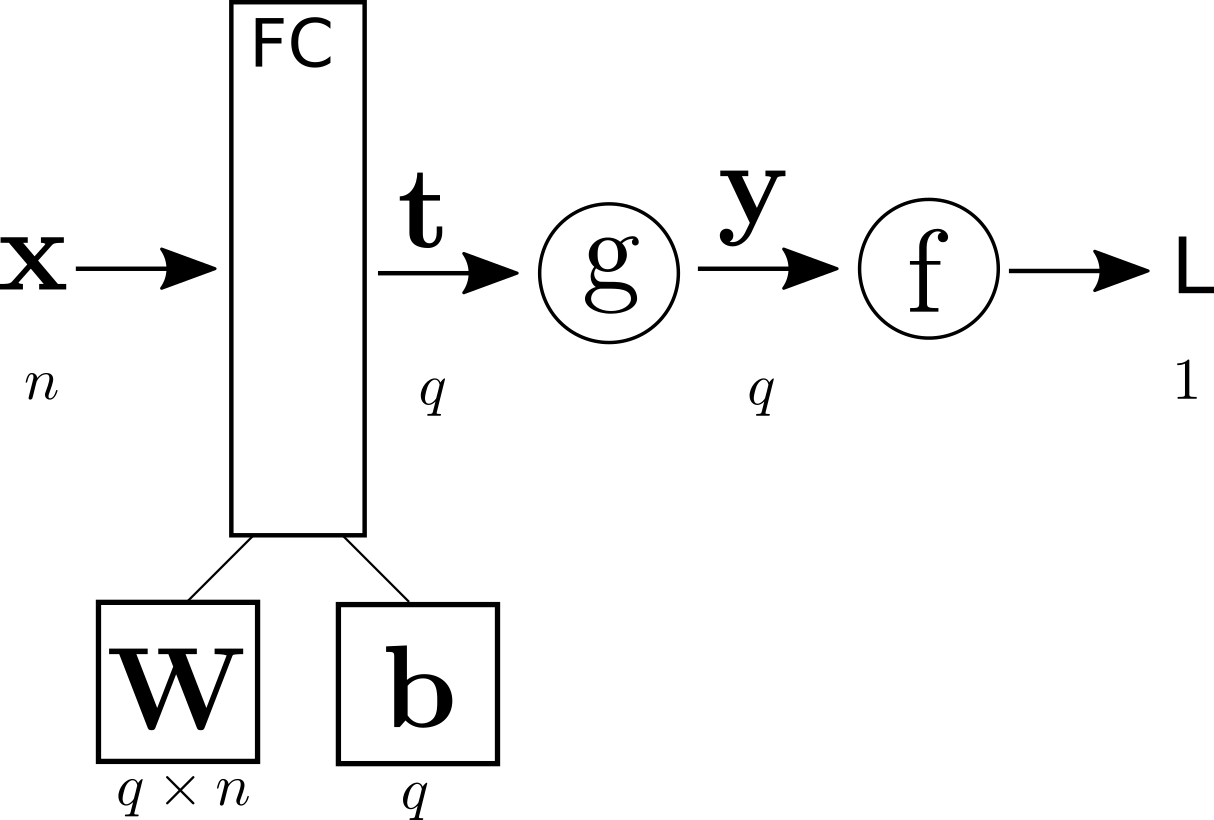
\includegraphics[width=0.5\textwidth]{bp_fc.png}
\end{figure}

\begin{columns}
  \begin{column}{0.5\textwidth}
    Forward pass:
    \begin{eqnarray*}
      \mathbf{t} &=& \W\x + \bias \\
      \y &=& \act(\W\x + \bias) \\
      \loss &=& \loss(\y)
    \end{eqnarray*}
  \end{column}

  \begin{column}{0.5\textwidth}
    Local gradients:
    \begin{eqnarray*}
      \pdv{\mathbf{t}}{\W} &=& \x^t \\
      \pdv{\mathbf{t}}{\bias} &=& 1 \\
      \pdv{\y}{\mathbf{t}} &=& \act'
    \end{eqnarray*}
  \end{column}
\end{columns}

\end{frame}

%%%%%%%%%%%%%
\begin{frame}{Backpropagation through a fully connected layer}
  \begin{figure}
    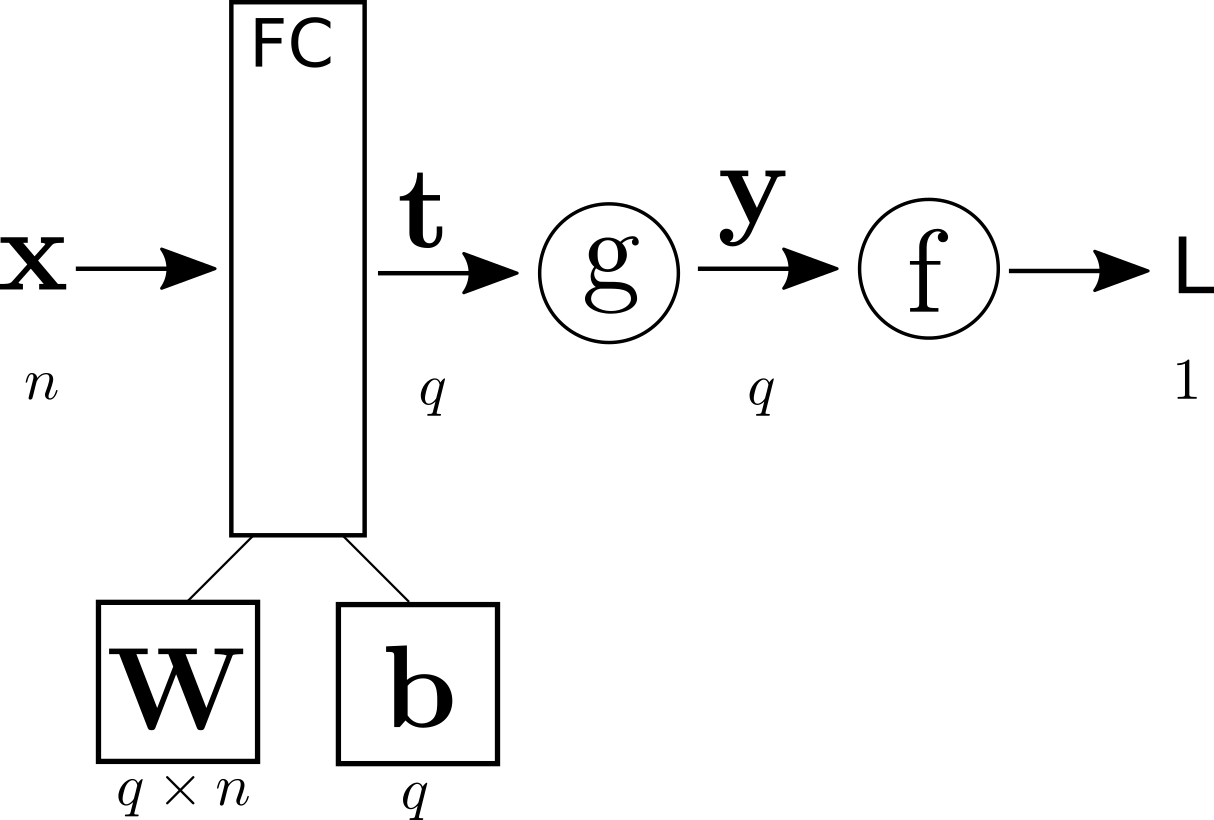
\includegraphics[width=0.5\textwidth]{bp_fc.png}
  \end{figure}

  Backpropagation:
  \begin{eqnarray*}
    \pdv{\loss}{\mathbf{t}} &=& \pdv{\loss}{\y}.\pdv{\y}{\mathbf{t}} \\
                           &=& \pdv{\loss}{\y} \odot \act'(\mathbf{t}) \\
  \end{eqnarray*}

\end{frame}

%%%%%%%%%%%%%
\begin{frame}{Backpropagation through a fully connected layer}
  \begin{figure}
    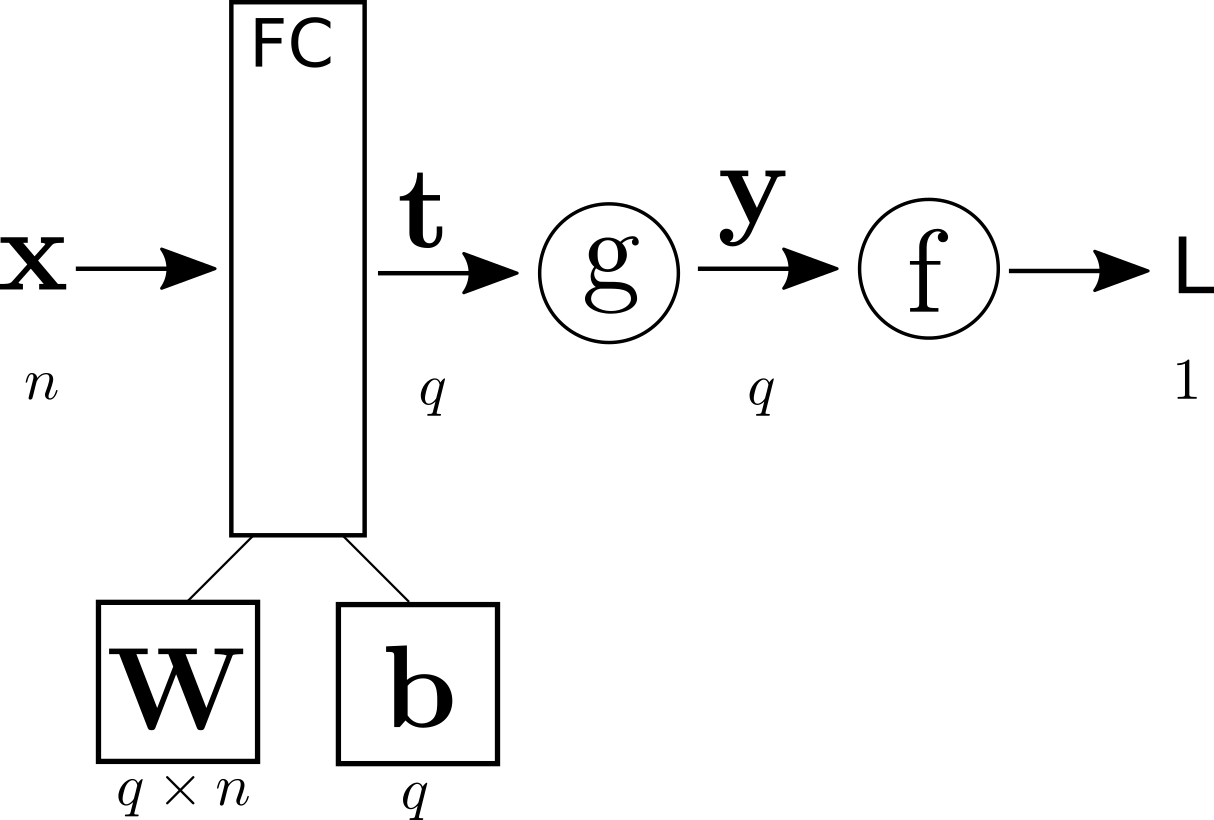
\includegraphics[width=0.5\textwidth]{bp_fc.png}
  \end{figure}

  Backpropagation:
  \begin{columns}
    \begin{column}{.5\textwidth}
      \begin{eqnarray*}
        \pdv{\loss}{\W} &=& \pdv{\loss}{\mathbf{t}}.\pdv{\mathbf{t}}{\W} \\
                   &=& \pdv{\loss}{\y} \odot \act'(\mathbf{t}).\x^t
      \end{eqnarray*}
    \end{column}

  \begin{column}{.5\textwidth}
  \begin{eqnarray*}
    \pdv{\loss}{\bias} &=&  \pdv{\loss}{\y} \odot \act'(\mathbf{t})
  \end{eqnarray*}
  \end{column}
\end{columns}


\end{frame}


%%%%%%%%%%%%%%%%%%%%%%%%%%%%%%%%%%%%
\begin{frame}{Network parameters initialization}

\begin{block}{General idea}
          Inputs of activation functions should be in an appropriate range (high gradient)
\end{block}

  \begin{columns}
    \begin{column}{.4\textwidth}
      \begin{figure}[ht]
        \centering
        \includegraphics[width=0.7\textwidth]{act_sigm.png}
      \end{figure}

      \begin{figure}[ht]
        \centering
        \includegraphics[width=\textwidth]{network}
      \end{figure}

    \end{column}

    \begin{column}{.6\textwidth}
        \begin{itemize}
        \item If all parameters are initialized to zero, then in each layer the activations will remain equal -- symmetry will never be broken
        \item Simple solution: random values from a normal or uniform distribution
        \item More advanced solutions exist: \cite{lecun_efficient_1998,glorot_understanding_2010,he_delving_2015}
        \end{itemize}
    \end{column}
  \end{columns}
\end{frame}

%%%%%%%%%%%%%%%%%%%%%%%%%%%%%%%%%%%%%%%%%%%%%%%%
%% \section{Application of fully-connected networks to image classification}

%% %%%%%%%%%%%%%%%%%%%%%%%%%%%%%%%%%%%%
%% \begin{frame}{Images}

%%   \begin{columns}
%%     \begin{column}{.5\textwidth}
%%       \begin{block}{Definition}
%%         \begin{itemize}
%%         \item Classically, an image is a matrix of values belonging to $[0, \ldots, 255]$ (grey level images) or to $[0, \ldots, 255]^3$ (color images).
%%         \item More generally, an image is a $q$-dimensional array of values belonging to $R^d$.
%%         \end{itemize}
%%       \end{block}

%%     \end{column}

%%     \begin{column}{.5\textwidth}
%%       \begin{figure}
%%         \centering
%%         \includegraphics[width=4cm]{faune.png}
%%       \end{figure}

%%     \end{column}
%%   \end{columns}

%% \end{frame}


%%%%%%%%%%%%%%%%%%%%%%%%%%%%%%%%%%%%
\begin{frame}{Conclusion}

  We have seen:
  \begin{itemize}
  \item What is an artificial neuron and an artificial neural network (NN)
  \item The (potential) power of a NN
  \item The backpropagation algorithm
  \item NN learning basics
  \end{itemize}

In the following, we will see how to process images using NNs.

\end{frame}


%%%%%%%%%%%%%%%%%%%%%%%%%%%%%%%%%%%%%%%%%%%%%%%%%%
\section*{References}

%%%%%%%%%%%%%%%%%%%%%%%%%%%%%%%%%%%%%%%%%%%%%%%%%%

\frame[allowframebreaks]{

\scriptsize

\frametitle{References}

%\bibliographystyle{amsalpha}
%\bibliographystyle{apalike}

\bibliography{edf.bib}

\normalsize

}

%%%%%%%%%%%%%%%%%%%%%%%%%%%%%%%%%%%%%%%%%%%%%%%%%%
%%%%%%%%%%%%%%%%%%%%%%%%%%%%%%%%%%%%%%%%%%%%%%%%%%
%%%%%%%%%%%%%%%%%%%%%%%%%%%%%%%%%%%%%%%%%%%%%%%%%%

\end{document}
